\documentclass[11pt]{report} 

%%%%%%%% Packages %%%%%%%%%%
\usepackage{graphicx, amsmath, amsfonts, amssymb, amsthm, pgfplots, tikz, siunitx, float, array, longtable}
\usepackage[top=2.5cm, left=3cm, right=3cm, bottom=3cm]{geometry} % Set margins
\usepackage[ruled,linesnumbered,lined,boxed,commentsnumbered, nofillcomment]{algorithm2e}
\usepackage{appendix}
\usepackage[
backend=biber,
style=ieee,
sorting=nyt
]{biblatex}
\addbibresource{sources.bib}

% Graph colours
 \usetikzlibrary{
        pgfplots.colorbrewer,
    }
\pgfplotsset{width=11cm,compat=1.9}
\pgfplotsset{
        % define a `cycle list' for marker
        cycle list/.define={my marks}{
            every mark/.append style={solid,fill=\pgfkeysvalueof{/pgfplots/mark list fill}},mark=*\\
            every mark/.append style={solid,fill=\pgfkeysvalueof{/pgfplots/mark list fill}},mark=square*\\
            every mark/.append style={solid,fill=\pgfkeysvalueof{/pgfplots/mark list fill}},mark=triangle*\\
            every mark/.append style={solid,fill=\pgfkeysvalueof{/pgfplots/mark list fill}},mark=diamond*\\
        },
    }


\setlength{\parindent}{0pt}

% Sections counters
\renewcommand\thesection{\arabic{section}}
\setcounter{secnumdepth}{3}


\begin{document}

%%%%%% Title Page %%%%%%%%%
\begin{titlepage}
    \begin{center}
        % NCL LOGO
        
\includegraphics[scale=0.07]{Components/Newcastle-University-Logo.png}    

        % TITLE
        \LARGE
        \textbf{The Graph Colouring Problem: Studying the efficiency and efficacy of constructive graph colouring algorithms}   
        \vspace{1.5cm}

        % AUTHOR
        \Large 
        \textbf{Harry Hainsworth-Staples \\ (190375508)}  \\ 
        \vspace{0.5cm}
        \textbf{Supervisor: Dr. Konrad Dabrowski}
        
            
        \vfill
        
        % WC + Extra Info
        \textbf{Word Count: [13,288]} 
        \vspace{0.5cm}

        For the award of Master of Science in Computer Science
            
        \vspace{0.5cm}
        
        School of Computing\\
        Newcastle University\\
        August 2024
            
    \end{center}
\end{titlepage}
\newpage
%%%%%%%%%%%%%%%%%%%%%%%%%%
\pagenumbering{roman}

%%%%%% Declaration %%%%%%%
\section*{Declaration}
This dissertation for the award of MSc in Computer Science is comprised solely of my own work, and has not been submitted, in part or in whole, for any other degree. Except where stated specifically otherwise, by reference or acknowledgement, this work is completely my own.

%%% Acknowledgements %%%%%
\section*{Acknowledgements}
I would like to thank Dr. Konrad Dabrowski for all his help and support as my supervisor for this project. I would also like to thank my family and in particular my partner Hollie for her constant support throughout my MSc.
\newpage
%%%%%% Abstract %%%%%%%%%%
\section*{Abstract}
The Graph Colouring Problem (GCP) is one of the best known problems in the field of Graph Theory, with significant applications in scheduling, timetabling, and register allocation to name a few. This project investigates the efficiency and efficacy of several constructive algorithms designed to provide upper bound solutions to the GCP. The algorithms include: GREEDY, WELSH-POWELL, DSATUR and RLF (Recurscive Largest First). The GREEDY algorithm was implemented using two variations based on vertex ordering heuristics. 
\\\\
This study evaluates the performance of each of these algorithms through extensive testing on multiple different graph instances, including randomly generated $G(n, p)$ graphs and standard benchmarks such DIMACS test instances with known $\chi(G)$. The results find that no single algorithm outperforms all the others in all contexts. RLF proves to be most efficacious at colouring large and dense graphs, however it is by far the least efficient. DSATUR excels in colouring small and sparse graphs, however again it is the second least efficient. GREEDY and WELSH-POWELL prove to be the most efficient algorithms however they are also the least and second least efficacious respectively. 
\\\\
This research highlights the trade-offs between algorithmic efficiency and the quality of solution generated. This project also provides a computer program that users can interact with to test the included algorithms on test instances.

%%%% Contents %%%%%%%%%%%%%
\tableofcontents
\listoffigures
\listoftables
\clearpage


%%%%%% MAIN BODY %%%%%%%%%%
\pagenumbering{arabic}

\section{Introduction}
The Graph Colouring Problem (GCP) is widely regarded as one of the most famous problems in the field of Graph Theory, with a history that dates back to 1852 with the problem of map colouring and the formulation of the Four-Colour Theorem (FTC) \cite{kubale2004}. The Four-Colour Problem (FCP) remained unsolved for over a hundred years, with one proof presented by A. B. Kempe \cite{Kempe4Color} later found to contain a mistake. A valid proof for the theorem was not formulated until 1976 by the work of K. Appel and W. Haken \cite{AppelHaken4Colour} which was, although controversially at the time, the first case of a computer assisted proof. This development made clear the power of computing as both an engine of searching the problem space and assisting in providing solutions to combinatorial optimisation problems \cite{kubale2004}. There are variations on graph colouring, including colouring the edges or the faces of a graph. However, this project will only be looking colouring the vertices of a graph. 
\\\\
In real-world contexts the GCP is often used as an abstraction for many different problems. One common example is timetabling, whereby it is important to use the minimal number of time periods whilst allowing students to take their desired classes \cite{DEWERRA1985151, Leighton1979AGC, LewisR.M.R2015AGtG, WelshPowell}. Another example is that of computer register allocation for improving the efficiency of compiling computer programs \cite{CHAITIN198147, LewisR.M.R2015AGtG}. The problem of scheduling is also often abstracted to that of graph colouring, with some examples being that of sports scheduling \cite{LEWIS2011190} and scheduling taxis \cite{LewisR.M.R2015AGtG}. In fact, any problem that involves reducing the input into a minimal number of distinct sets so that no conflicts within sets are created, can be thought of as a GCP. Perhaps the most common GCP that most people will have encountered is the game Sudoku.
\\\\
There are various different algorithms that can be used to provide solutions to the GCP. However, depending on the context, a particular algorithm may be better suited than another. For example, if efficiency is not a concern, the focus would be on using the most efficacious algorithm to find the solution. However, if efficiency is a concern, the algorithm providing the most efficacious solution may not necessarily be the most appropriate. Therefore, it is important for those facing GCP to understand to benefits and drawbacks of the various constructive colouring algorithms that could be used within their circumstances. 
\\\\
The current project is about implementing various constructive algorithms that provide solutions to the GCP and measuring their efficiency and efficacy in tackling the problem. The results of this project could provide indication of the most efficient and efficacious algorithms for certain contexts, which in turn could be implemented to provide solutions to the real-world problems identified above. 

\subsection{Aim}
The aim of this project is to study various constructive techniques developed to find solutions to the GCP. This project aims to implement four such algorithms namely: GREEDY, WELSH-POWELL, DSATUR and RLF (Recursive Largest First). The GREEDY algorithm will be implemented with two variations in vertex ordering heuristics attempting to colour them either: in the order they are read; or in a pseudo-randomly generated order (vertices are shuffled using a random number generator). The WELSH-POWELL algorithm will have two implementations with one building off the GREEDY approach, however initially ordering the vertices by their degree (number of neighbours). The second WELSH-POWELL implementation will also use the approach of sorting vertices by their degree, although there will be some extra bookkeeping involved in building up each colour set. 
\\\\
This project aims to test these various constructive colouring techniques on a range of problem instances. This will allow more general conclusions and understanding to be made about the performance metrics of each algorithm, rather than testing on a particular graph that may contain advantages for a particular heuristic. Therefore, each algorithm is aimed to be tested on a range of known graphs varying in order and size, taken from DIMACS’ second implementation challenge \cite{DIMACSChallenge2}, and also randomly generated graphs varying in order and p-value, where p is the probability that an edge will be created between two vertices. 
\\\\
The project will focus on two metrics to compare and study these constructive algorithms. Metric one is the algorithms efficacy in colouring a graph. Efficacy in this case being defined as the quality of colouring an algorithm produces on average over multiple runs. The quality is determined by how few colours an algorithm uses in colouring, or, in other words, how close to the optimal chromatic number of colours was used. For graphs where the chromatic number is unknown the efficacy of an algorithm will be determined by comparison with the other algorithms (i.e. one that produces a smaller $k$-colouring will be deemed more effective). The second metric is the algorithms efficiency in colouring. There are many ways to measure efficiency of a computer algorithm, perhaps most common would be to simply measure the time taken for a solution to be reached. As Lewis points out however, this is very hardware and language specific, two different computers may take vastly different times to run the same algorithm due to hardware constraints \cite{LewisR.M.R2015AGtG}. Similarly, an algorithm written in a very efficient language such as C++ would likely run a great deal faster than one written in a higher-level language such as Python. With all that being said, there is still some insight that can be gained from measuring time taken, providing that each of those variables are kept constant throughout the results gathering process. Therefore, accompanying the timing metric for efficiency, as suggested in the work of Lewis \cite{LewisR.M.R2015AGtG},  this project will also use  the number of operations performed by an algorithm during its execution as a measure of computational cost i.e. efficiency.
\\\\
The hypotheses of the project are as follows:
\begin{enumerate}
    \item The RLF algorithm will prove most effective in colouring, particularly for larger and more dense graphs.
    \item The DSATUR algorithm will be the second most effective and may prove most effective for smaller, and sparser graphs.
    \item The WELSH-POWELL algorithm will prove slightly more effective than both GREEDY approaches. However, they will all prove less effective than RLF and DSATUR.
    \item RLF will be the least efficient due to the greater number of checks it must conduct in finding solutions. This will likely be followed by DSATUR, and then WELSH-POWELL, with GREEDY proving the most efficient. 
\end{enumerate}

\subsection{Objectives}
The following objectives have been set out in order to complete the previously laid out project aims:
\begin{itemize}
    \item Conduct a literature review into graph colouring, the graph colouring problem and various constructive techniques employed in solving the graph colouring problem
    \item Implement four constructive graph colouring algorithms being: GREEDY, DSATUR, WELSH-POWELL, and RLF
    \item Implement a method of reading in graph instances for the algorithms to run on
    \item Implement a way to generate random graphs for the algorithms to run on
    \item Thoroughly test the software to ensure it is working as expected and the validity of the results being generated
    \item Visualise and discuss the results generated from running the algorithms on multiple known and random graph instances
\end{itemize}
	
\subsection{Project Scope}
While the focus of this project is primarily an exploration into the mentioned constructive algorithms by measuring and comparing their respective efficacy in colouring and efficiency in performance, it also aims to produce a piece of software. It is therefore necessary to highlight and follow the steps of software development. This section, therefore, aims to define the scope of the resultant software produced to measure the graph colouring algorithms. The first section defines the functionality to be included. The final section defines functionality that could be considered given the purpose of the software but will not be included in this particular iteration of development. Although out of scope for this phase of development, they could be considered as possible future extensions and areas of further research.
\subsubsection{In Scope}
\begin{itemize}
    \item Functionality to read in DIMACS graphs
    \item Functionality to print results to a chosen destination file
    \item Functionality to generate random graphs
    \item Functionality to run a graph colouring algorithm on a given graph, algorithms to be implemented are as follows:
    \begin{itemize}
        \item GREEDY using the following vertex ordering heuristics:
        \begin{itemize}
            \item In order as read in from a DIMACS file
            \item Randomly shuffled 
        \end{itemize}
        \item WELSH-POWELL (with the two mentioned variations)
        \item DSATUR 
        \item RLF (Recursive Largest First) 
    \end{itemize}

\end{itemize}
\subsubsection{Out of Scope}
\begin{itemize}
    \item Any other graph colouring approaches such as backtracking or hybrid meta-heuristics
    \item Auto result visualisations 
    \item Implementation of a GUI
\end{itemize}

\subsection{Motivation}
As alluded to within the introduction, the GCP is a very active area of research in both Mathematics and Computer Science alike. Its intractability and complexity, provide intrigue, while its applications prove immensely valuable. Indeed, as R. Beigel and D. Eppstein stated in their paper on 3-colouring: 
\begin{quote}
    \textit{"Unless P = NP, we know that no polynomial time algorithm for these problems can exist, but that does not obviate the need to solve them as efficiently as possible, indeed the fact that these problems are hard makes efficient algorithms for them especially important."}\cite{BEIGEL2005168}
\end{quote}
This dissertation seeks to understand and use the more easily comprehensible (and useful for finding upper bounds of the chromatic number) constructive colouring algorithms. This will allow for a better personal understanding of the field and provide a pathway to further research perhaps closer to the cutting edge of graph colouring research. 

\subsection{Outline of Project}
	
This dissertation is comprised of six sections which provide coherence and a sense of logical development in the sense that each section will flow logically from another from understanding the problem, execution, visualisation of results, and finally understanding, analysing, and placing those results. 
\\\\
The current section provides context regarding the GCP and outlines the aims, objectives and scope of the project. Section two provides more in-depth background surrounding the GCP and the techniques and heuristics this project employs to find solutions. Furthermore, section two looks at some of the techniques used within the graph colouring field for measuring the performance and efficacy of particular algorithms. The third section presents the approach taken during the development of the graph colouring software, including software engineering techniques, such as design, implementation, and testing strategy where appropriate. Section four provides the results obtained from running the various implemented algorithms on both known test graphs from the second DIMACS implementation challenge \cite{DIMACSChallenge2}, and also randomly generated graphs. This section will finish by discussing the results obtained and reflecting as to whether they meet the expectations set out in the current section. It also considers how the results place and compare with other findings within the field. The fifth section will reflect on the project approach and method set out in section 3. This section will discuss how well the final product matched the requirements and objectives set out by the project. The final section looks to summarise and critique the project as a whole with consideration of areas for improvement and acknowledgement of successes. Finally, it will look retrospectively at what has been learned through this process and present possible areas for future follow-on research. 

\section{Background Research}
The aim of this project is to implement several constructive graph colouring algorithms and compare them through the previously established metrics of efficacy and efficiency. This section will explore the Graph Colouring Problem (GCP) as a whole and introduce key concepts and notation. It will explore the complexity of the problem, as well as covering how to translate a graph into a format that a computer can understand and manipulate. Then, each algorithm to be implemented within this project will be explored. Particular focus will be paid to its origins, how it works, and its complexities. After that, this section will look at the graph testing instances that can be used to test these algorithms.


\subsection{The Graph Colouring Problem}
As outlined in section 1, the GCP has its history in map colouring and the FCP. The aim of the FCP is to colour each region of a map so that no two neighbouring regions share the same colour. The FCT postulated that for any map only four colours are required which, as mentioned previously, was then proven to be true \cite{AppelHaken4Colour}. 
\\\\
A map can be imagined as a planar graph with the central point of each region being a vertex and each neighbouring region being connected with an edge (a planar graph being one that can be drawn within the plane, i.e. there is a version of the graph that can be drawn on a two-dimensional plane whereby no two edges cross over). The aim being to colour each node so that no two neighbouring vertices (i.e. those connected by an edge) are assigned the same colour. An optimal solution (always being four for planar graphs) would be to use the minimal number of colours.
\\ \\
This leads nicely on to the GCP as whole, as an extension of the FCP, which includes non-planar graphs. The basic aim of the problem remains the same: to colour each vertex of the graph so that no connected vertices have the same colour all while minimising the number of colours being used. A valid colouring of a graph $G$ is one that follows the first aim of colouring by containing no conflicts between vertices. Colouring $G$ using $k$ colours means that $G$ is $k$-colourable. An optimal colouring of G is one that uses the minimum number of colours. This is referred to as the chromatic number and is notated by the Greek letter Chi. In other words, an optimal colouring of $G$ is one whereby $k = \chi(G)$.


\subsection{Problem Complexity}
There are many algorithmic approaches to finding solutions to the GCP, however none of these can claim to “solve” the GCP. As Lewis states, to solve the GCP would be to take any graph of any size or topology and return the optimal solution (i.e. a colouring whereby $k = \chi(G)$) in all cases \cite{LewisR.M.R2015AGtG}. Due to work by Stephen Cook on Complexity Theory and introducing ideas of NP-completeness and problem reductions, the GCP can be said to be NP-complete as it can be reduced from the Satisfiability Problem that Cook proved to be NP-complete \cite{Cook1971}. 
\\\\
The idea of P and NP stems from the field of Complexity Theory used to categorise problems into sets based upon their complexity. This theory states that there are two ways of looking at problems. The first way is to frame the problem as a searching problem in which the aim is to find a solution to a given instance. The second way would be to frame it as a decision problem to which the answer is either "yes" or "no" and the problem is looking if an instance has a certain property \cite{Goldreich_2010}. P is the set containing problems for which there are algorithms that can efficiently solve it, whereas NP contains the set of problems that have efficiently verifiable proofs for solutions that claim a "yes" answer \cite{Goldreich_2010, LewisR.M.R2015AGtG}. Posing a problem as a searching problem or a decision problem comes mainly down to how the problem is stated. For example, the GCP could be posed as a searching problem in the form: "Given a graph $G$ what is the minimum number of colours required to colour $G$?". On the other hand it could be posed as a decision problem, as Lewis proposes, in the form: “Can a graph $G$ be coloured feasibly using $k$ colours?” \cite{LewisR.M.R2015AGtG}. The GCP as a whole is said to be intractable because an algorithm that could answer either of those questions is not feasible within polynomial-time, however, when presented with a solution, it would be feasible to determine its correctness, providing it is claiming "yes" in the decision variation. 
\\\\
Previous work has suggested that constructing an algorithm that could claim to "solve" the GCP seems to be insoluble theoretically and practically \cite{WelshPowell}. However, there are several algorithms that can provide both upper and lower bound approximations of the chromatic number \cite{MaxClique, MaxClique2, CulbersonColoring, LEWISHillClimber}. With so many options out there that can provide solutions to the GCP, it is important to understand which is best. Therefore, it is important to establish solid metrics to compare how algorithms perform in contrast to others. In computing there are several notations that are used to characterise an algorithms performs in terms of efficiency. Perhaps the most commonly used is that of big $O$ notation. $O$-notation provides an upper bound to an algorithms asymptotic behaviour, or in other words it states that the computational complexity grows no faster than the highest order term of the function that defines it \cite{IntroAlgs}. For example an algorithm might be defined by a rate $4n^2 + 4n + 2$, where $n$ is the size of the input provided. However, as $n$ grows and tends towards infinity the only part of that equation with any consequence becomes $n^2$. Therefore, using $O$-notation the complexity of the algorithm is $O(n^2)$. There are also other notations that provide lower bounds, and tight bounds \cite{IntroAlgs}. However more generally, there is a greater interest in knowing the worst case scenarios. 
\\\\
While $O$-notation is very useful for providing theoretical insight into an algorithms performance, it remains just that: a theoretical upper bound or worst case. Practically speaking, testing on very large inputs becomes unfeasible due to the necessity of either immense computing power or impractical amounts of time. It is therefore useful to test algorithms on real-world problem instances to gauge how they perform. To achieve this, it is necessary to have some practical metric to measure the algorithms efficiency. Perhaps the most obvious measurement would be to simply measure the time taken for the algorithm to complete its execution \cite{Kronsjo, Leighton1979AGC}. However, it has been shown that timing using methods, such as the CPU clock, mean the result is very much hardware or programming language dependant \cite{Eiben, LewisR.M.R2015AGtG}. It has been stated that using a more hardware and implementation independent method for measuring algorithms, such as the number of atomic operations used by the algorithm to find a solution, might be more suitable \cite{Eiben, LewisR.M.R2015AGtG}.  

\subsection{Representing Graphs}
There are generally two standard ways of representing graphs: an Adjacency List, or an Adjacency Matrix \cite{LewisR.M.R2015AGtG, IntroAlgs}. An Adjacency List representation commonly uses an array structure to store lists of neighbouring vertices. For example, given a graph $G = (V, E)$ where $V$ is the set of vertices and $E$ is the set of edges. An array $Adj$ of length $|V|$ would be constructed so that for each vertex $v \in V$ the list $Adj[v]$ would contain a list of all the neighbouring vertices $u$ so that $(v, u) \in E$ \cite{IntroAlgs}. Therefore, if given an edge set $\{(v_{1}, v_{2}), (v_{1}, v_{3}), (v_{2}, v_{3}), (v_{3}, v_{4}), (v_{3}, v_{5})\}$ and Adjacency List representation would be:
\begin{equation*}
     \begin{bmatrix}
    v_{1} \rightarrow \{v_{2}, v_{3}\}, \\
    v_{2} \rightarrow \{v_{1}, v_{3}\}, \\
    v_{3} \rightarrow \{v_{1}, v_{2}, v_{4}, v_{5}\}, \\
    v_{4} \rightarrow \{v_{3}\}, \\
    v_{5} \rightarrow \{v_{3}\}, \\
    \end{bmatrix} 
\end{equation*}
An Adjacency List has the desirable property of being memory efficient as only existing edges are stored within memory and has a space complexity of $O(V + E)$ \cite{IntroAlgs}. This is particularly desirable for sparse graphs. Furthermore, iterating over neighbouring vertices is dependant on the degree of the vertex as each list only contains neighbouring vertices. This operation therefore has a time complexity of $O(deg(v))$.
\\\\
On the other hand, an Adjacency Matrix representation of $G$ uses a $|V| \times |V|$ matrix $A$ whereby for vertices $v$ and $u$, $A[v][u] = 1$ if and only if $(v, u) \in E$, otherwise it is 0 \cite{IntroAlgs}.  Therefore, an Adjacency Matrix of the edge set established earlier would look like:
\begin{equation*}
     \begin{bmatrix}
     0 & 1 & 1 & 0 & 0 \\
     1 & 0 & 1 & 0 & 0 \\
     1 & 1 & 0 & 1 & 1 \\
     0 & 0 & 1 & 0 & 0 \\
     0 & 0 & 1 & 0 & 0 \\
    \end{bmatrix} 
\end{equation*}
The space complexity of an Adjacency Matrix is less desirable than the Adjacency List as it is always $O(V^2)$ regardless of the number of edges \cite{IntroAlgs}. This is particularly wasteful for sparse graphs as it means storing redundant information. Furthermore, finding the neighbours of a vertex requires iterating over all the vertices to check if it is a neighbour or not (i.e. checking if it is 0 or 1). This operation therefore has a time complexity of $O(V)$.

\subsection{The GREEDY algorithm}
The GREEDY algorithm, sometimes referred to as FIRST-FIT algorithm, is one of the earliest heuristics developed in finding solutions to the GCP \cite{LEWIS20121933}. The GREEDY algorithm is perhaps one of the simplest algorithms for graph colouring, however it is also perhaps the most fundamental \cite{LewisR.M.R2015AGtG}. The algorithm works by taking in vertices in some order and assigning each vertex the first colour it can without creating any conflicts \cite{LewisR.M.R2015AGtG}. It can be thought of as:
\begin{verbatim}
    1. Given a Graph G with a vertex set V assign the first vertex v in 
       V with a colour 0.
    2. Take the next vertex in V and assign it the first colour that does 
       not create any conflicts, creating new colours where necessary (add 
       1 to previous colour).
    3. Repeat step 2 until all vertices in V are assigned a colour.
\end{verbatim}
It has been shown that there is always an ordering of the vertices whereby the GREEDY algorithm can produce the optimal solution \cite{LewisR.M.R2015AGtG}. This is where the idea of the SHUFFLED GREEDY algorithm comes in. Prior to step 1 (shown above), the vertices are shuffled into a random order. Therefore, repeating the SHUFFLED GREEDY algorithm will eventually produce a solution that is optimal. However, as the graph becomes larger the chances of this happening become astronomical. This is because the number of ways the vertices can be ordered is calculated by $|V|!$, which quickly gets out of hand as the number of vertices grows. It therefore becomes extremely unlikely that the algorithm will stumble upon the optimal ordering. It has been shown that the worst case complexity of the GREEDY algorithm is $O(n^2)$ \cite{LewisR.M.R2015AGtG}.

\subsection{The WELSH-POWELL algorithm}
The WELSH-POWELL algorithm is one of the earliest heuristics proposed for the ordering of vertices building off of the GREEDY approach \cite{LEWIS20121933}. The work of Welsh and Powell suggests that vertices should be sorted according to their degrees, with the highest degree coming first \cite{WelshPowell}. Therefore, the WELSH-POWELL algorithm is simply the GREEDY algorithm with the extra step of sorting first. It has been shown that sorting has a complexity of $O(n \log n)$ (where $n$ in this case is the number of vertices) \cite{IntroAlgs}. This means that, in the worst case, WELSH-POWELL still has a complexity of $O(n^2)$. However, practically the extra step of sorting will make a slight impact in its efficiency comparable to GREEDY. 
\\\\
There is also a slight variation proposed of the WELSH-POWELL algorithm that aims to build colour sets rather than iteratively going through each vertex \cite{GFGWP}. This variation goes as follows:
\begin{verbatim}
    1. Sort the vertices in order of degree (highest first).
    2. Colour the first vertex with colour 0.
    3. Proceed to assign this colour to all uncolored vertices not 
       connected to the vertex.
    4. Increment the colour.
    5. Assign the next vertex with highest degree with the new colour.
    6. Repeat steps 3 - 5 untill all vertices have been coloured. 
\end{verbatim}
This variation will be used within the project to allow for comparisons to be made between the two variations. 

\subsection{The DSATUR algorithm}
The DSATUR algorithm was first proposed by Br\'{e}laz and gets its name from an abbreviation of degree of saturation \cite{BrelazDSatur}. In essence the GREEDY method and DSATUR are very similar in that they aim to assign each vertex with the minimum colour on each iteration. However, whereas GREEDY has a predetermined ordering, DSATUR decides heuristically which vertex to colour next based upon the most constrained vertices with highest saturation \cite{LewisR.M.R2015AGtG}. The degree of saturation of a vertex $v$ that has not yet been coloured is determined by the number of different colours assigned to neighbouring vertices of $v$ \cite{BrelazDSatur, LewisR.M.R2015AGtG}. The algorithm as set out by Br\'{e}laz \cite{BrelazDSatur} is as follows:
\begin{verbatim}
    1. Sort the vertices by order of degree (highest first).
    2. Colour the vertex of maximal degree with the first colour.
    3. Choose the next uncoloured vertex of maximal saturation degree. 
       If there is a tie, choose any vertex of maximal degree.
    4. Colour the chosen vertex with the minimal possible colour.
    5. If all vertices are coloured stop, if not return to step 3.
\end{verbatim}
In the same work, Br\'{e}laz also showed that DSATUR is exact for bipartite graphs \cite{BrelazDSatur}. Bipartite graphs are a special topology of graph whereby the vertices are within two distinct sets, and no vertices within those sets share an edge. A bipartite graph can be defined as a graph that contains no cycles, and a bipartite graphs optimal colouring is always two (i.e. $\chi(G) = 2$) \cite{LewisR.M.R2015AGtG}. It has also been shown that DSATUR is exact for other fundamental graph topologies such as cycle and wheel graphs \cite{LewisR.M.R2015AGtG}. The worst case complexity of DSATUR, much like GREEDY, has been shown to be $O(n^2)$ \cite{LewisR.M.R2015AGtG}. However, in practice DSATUR is less performative than GREEDY due to the complexity added by the degree of saturation heuristic. 

\subsection{The RLF algorithm}
The RLF algorithm was designed by Leighton to solve large scheduling problems \cite{Leighton1979AGC}. Unlike previous algorithms that colour vertices one by one, RLF colours the graph one colour at a time \cite{LewisR.M.R2015AGtG}. Each iteration of the algorithm aims to build up an independent set of vertices that is then associated with a colour. Much like the approach of DSATUR, RLF also looks to tackle the most constrained vertices first. Similar to in DSATUR, the first vertex $v$ chosen for each colour set being constructed is that of the highest degree within the set of uncoloured vertices \cite{Leighton1979AGC, LewisR.M.R2015AGtG}. All neighbours of $v$ are then removed from consideration. Where RLF differs from DSATUR is in the choice of the next vertex to be coloured in the remaining sub-graph, induced by removing all the neighbours of $v$. The next vertex $u$ is chosen whereby $u$ is the one with the largest number of neighbours within the subgraph of the removed vertices of $v$ \cite{Leighton1979AGC}. The algorithm can be thought of as follows:
\begin{verbatim}
    1. Set the colour to 0.
    2. Take an uncoloured vertex v whereby it is the vertex with maximal 
       degree.
    3. Assign it with the current colour and remove it from the graph.
    4. Remove all the neighbours of v from the graph and for each vertex 
       remaining count the number of neighbours it has within the vertices 
       that have been removed.
    5. Choose the next vertex u that has the most neighbours from step 3.
    6. Assign it to the current color set and remove it from the graph.
    7. Repeat steps 3 - 5 until there are no more vertices left in the 
       graph.
    8. If all vertices are coloured stop, if not restore all uncolored 
       vertices to the graph increase the colour by 1 and go back to 
       step 2. 
\end{verbatim}
Unlike all the previous algorithms which have a worst case complexity of $O(n^2)$, Leighton showed that RLF has a worst case complexity of $O(n^3)$. However, he also showed that RLF can behave like $O(n^2)$ for sparse graphs \cite{Leighton1979AGC}. It has also been shown that RLF, like DSATUR, provides the optimal solution for many fundamental graph topologies including bipartite, cycle and wheel graphs \cite{LewisR.M.R2015AGtG}. 
\subsection{Test Instances}
When new algorithms for the GCP are proposed, it stands to reason to compare them with other existing methods. It is therefore important to have standard testing instances so that the performance of the algorithms can be easily compared. A development in 1992 helped in this regard with the the second DIMACS implementation challenge. This culminated in a suite of graph colouring test instances being released to the public domain \cite{DIMACSChallenge2}. Since this time, many researchers within graph colouring have used this testing set to tune their algorithms to achieve better results \cite{LewisR.M.R2015AGtG}. Some testing instances, also contained within the DIMACS set, of particular note are those proposed by Leighton in his work on RLF. He noted that much of the graph colouring testing was performed on randomly generated graphs, however none of them provided the chromatic numbers of the test graphs used \cite{Leighton1979AGC}. Leighton therefore proposed a new method for generating random test graphs with a known chromatic number \cite{Leighton1979AGC}. 
\\\\
Testing the algorithms on DIMACS instances provides insights of their performance on a particular problem set. However, to gain more general insights of the algorithms performance on a particular type of graph, the algorithms must be tested on many variations of graphs of that type. One method proposed for this is that of using randomly generated $G(n, p)$ graphs \cite{LewisR.M.R2015AGtG}. A random graph $G(n, p)$ is one that comprises of $n$ vertices and each pair of vertices has $p$ probability of being adjacent \cite{LewisR.M.R2015AGtG}. This allows for testing to be done by tweaking the edge probability $p$ and altering the randomly generated graphs from being sparse to dense. 


\subsection{Summary}
To summarise, after a review of the literature, it was decided to implement all the constructive algorithms discussed previously within a computer program. The idea then being to compare and contrast the efficacy and efficiency of the algorithms using the metrics established in section 2.2. The algorithms were to be tested upon the randomly generated $G(n, p)$ graph instances and DIMACS testing instances with known chromatic number as discussed in section 2.8. Each graph should then have the ability to be stored within both an Adjacency List and Adjacency Matrix and then provide a colouring solution by inputting it into one of the algorithms. Conclusions could then be made as to the most efficient method for storing graphs within memory. This all culminated in the decision to design and construct a piece of software that has the ability to take test instances and generate results that will provide insights into the efficacy and efficiency of all the algorithms. This software is thoroughly discussed in the next section. 
\section{Method}

The following section focuses on the approach taken to fulfill the aims of this project. Firstly, it will look at the requirements derived from the background research and will formulate those into some system requirements. Section 3.2 will look at the design of the program for colouring the graphs and some of the methods used to represent graphs and the algorithms in code. 
Section 3.3 will look closer at the implementation of the program as a whole. Finally, section 3.4 looks at methods of testing and the approach behind the results that were gathered. 
\\\\
As mentioned in previous sections the aim of this project is to create a program for colouring graph instances in DIMACS format, similar to that created by Lewis accompanying his guide to graph colouring \cite{LewisR.M.R2015AGtG}. However, this project will purely focus on constructive colouring algorithms and will include the ability to test on multiple DIMACS instance graphs along with randomly generated graph instances. Lewis' program used C++ as the choice of language to build up the application, however the choice for this project was Java. The choice of language is mainly arbitrary and dependant upon the preference of the developer. However, in this case Java provided particular advantages for this project. The first being that it is the most comfortable language for the author and developer, therefore making it a clear choice. The second reason for choosing Java is to take advantage of the Object-Oriented Programming (OOP) techniques (such as inheritance and abstraction) it provides in creating hierarchies to aid in representation of Graphs, Vertices and Edges. Java also has many inbuilt data-structures within the language that make the implementation of the algorithms quicker and simpler to understand. Overall, the choice mainly came down to the preference of the developer, although the choice of Java also provided some extra benefits in this case. 
\\\\
The development of this project will be completed using agile methodology. Due to the nature of the software being produced there may need to be modifications to the requirements and design during the development phase \cite{Agile}. Also, there is a limited time to complete this project therefore lengthier methodologies, such as waterfall, that involve strict phases of requirements gathering, design, implementation and testing did not seem appropriate in this case \cite{Waterfall}. Using agile will allow for tweaks within the design and requirements while simultaneously implementing and testing the software. Therefore, agile seemed the most appropriate methodology to adopt for this project. 

\subsection{Requirements}
System requirements are an important aspect of the software development process to determine the functionality of the system to be produced. Based on the background research in section 2, and considering the overall aim of the project, the following requirements should be considered in the design of the program as a whole:
\begin{itemize}
    \item Ability to read in graphs from input files in DIMACS format
    \item Ability to store the read in graphs in Adjacency List and Adjacency Matrix format
    \item Ability to colour these graphs using the constructive colouring techniques previously established
    \item Ability to gather results regarding number of colours used, number of operations, and time taken for each algorithm
    \item Ability to print these results to an output file
    \item Ability to generate random $G(n, p)$ graphs
    \item To have a simple User Interface (UI)
\end{itemize}

To include all of these requirements, and given the time constraints of the project, the program to be created will use a simple terminal UI. This will be the way a user can interact with the algorithms and will be used for the generation of the results in section 4 of this project.  

\subsubsection{Functional Requirements}
The functional requirements of the system represent the specific features expected of the system that will allow a user to accomplish the desired tasks. The features required of the UI are listed in the table below.

\begin{longtable}{|m{0.1\textwidth}|m{0.65\textwidth}|m{0.1\textwidth}|m{0.15\textwidth}|}
    \hline
    \textbf{Number} &  \textbf{Description} & \textbf{Priority} & \textbf{Comments} \\
    \hline
    FR1 & User can colour a single graph & High & See NFR1-2 \\
    \hline
     FR2 & User can colour a graph of their choice in DIMACS format using \textbf{GREEDY} algorithm & High & See NFR2 \\
     \hline
     FR3 & User can colour a graph of their choice in DIMACS format using \textbf{SHUFFLED GREEDY} algorithm & High & See NFR2 \\
     \hline
     FR4 & User can colour a graph of their choice in DIMACS format using \textbf{WELSH-POWELL1} algorithm & High & See NFR2 \\
     \hline
     FR5 & User can colour a graph of their choice in DIMACS format using \textbf{WElSH-POWELL2} algorithm & High & See NFR2 \\
     \hline
     FR6 & User can colour a graph of their choice in DIMACS format using \textbf{DSATUR} algorithm & High & See NFR2 \\
     \hline
     FR7 & User can colour a graph of their choice in DIMACS format using \textbf{RLF} algorithm & High & See NFR2 \\
     \hline
     FR8 & User can colour a graph of their choice in DIMACS format using all of the algorithms & High & See NFR2 \\
     \hline
     FR9 & User can generate results from testing all algorithms on DIMACS challenge instance graphs & High & See NFR3\\
     \hline
     FR10 & User can generate results from testing all algorithms on randomly generated $G(n, p)$ graphs & High & See NFR4\\
     \hline
     FR11 & User can generate a new random $G(n, p)$ graph & Medium & See NFR5 \\
    \hline
    FR12 & Users can choose to use algorithms with either adjacency list graphs or adjacency matrix graphs as input & Medium & \\
     \hline
     FR13 & User can exit the program & High & See NFR6\\
     \hline
\caption{Functional Requirements}
\label{tab:FuncReqs}  
\end{longtable}
  

\subsubsection{Non-Functional Requirements}
The non-functional requirements specify and describe the systems capabilities and constraints. These are listed in the table below. 

\begin{longtable}{|m{0.1\textwidth}|m{0.65\textwidth}|m{0.1\textwidth}|m{0.15\textwidth}|}
\hline
\textbf{Number} &  \textbf{Description} & \textbf{Priority} & \textbf{Comments} \\
\hline
NFR1 & The users will be provided with a menu to choose if they would like to: 
        \begin{enumerate}
            \item colour a single graph
            \item generate results from a set of DIMACS challenge instances
            \item generate results from a set random $G(n, p)$ instances
            \item generate a random $G(n, p)$ instance
            \item exit the program
        \end{enumerate}
        Any invalid input will ask for a reentry.
        & High & Satisfies FR1,9,10,11,12  \\
\hline
NFR2 & Users can colour a single graph using any of the implemented algorithms by:
        \begin{enumerate}
            \item selecting option 1 in the main menu
            \item inputting the file path of the graph to colour
            \item selecting which (or all) algorithm to use  
        \end{enumerate}
        If the graph is not in DIMACS format or cannot be found users will be asked to start again.
        Results will be printed to the terminal. Time taken to produce results will depend on size and density of input graph.
        & High & Satisfies FR1-8 \\
\hline
NFR3 & Results can be generated for DIMACS instances by selecting option 2 in the main menu. The user will then need to input the number of test runs required for each graph. The results will be printed to an output file and the name of the file printed to the terminal. Results will be gathered regarding number of colours used, number of operations and time taken. The time taken to complete generating results depends on the number of test runs desired. & High & Satisfies FR9 \\
\hline
NFR4 & Results can be generated for $G(n, p)$ graphs by:
    \begin{enumerate}
        \item selecting option 3 in the main menu
        \item input number of $G(n, p)$ graphs to generate per $p$-value
        \item input comma separated list of $p$-values
        \item input number of $n$
    \end{enumerate}
    Any invalid input the user will need to restart. Results will be printed to an output file and the name of the file will be printed to the terminal. Results will be gathered regarding number of colours used, number of operations and time taken. Time taken to complete generating results depends on number of graphs generated, number of $p$-values being tested and size of $n$.
    & High & Satisfies FR10 \\
\hline
NFR5 & A random $G(n, p)$ can be generated by:
    \begin{enumerate}
        \item selecting option 4 from the main menu
        \item input a value for $n$
        \item input a value for $p$
    \end{enumerate}
    Any invalid input the user will need to restart. The graph will be printed to an output file and the name of the file will be printed to the terminal. Generation should be almost instantaneous. 
    & High & Satisfies FR11 \\
\hline
NFR6 & Users can terminate the program by selecting option 5 in the main menu, termination will be instantaneous and will update any output files. & High & Satisfies FR13 \\
\hline
\caption{Non-Functional Requirements}
\label{tab:NonFuncReqs}
\end{longtable}
   
\subsection{Design}
The design of the program is split into three sections. The first of which is the Graph hierarchy that defines and stores the graphs in a manner that a computer can interpret. The second portion of the design focuses on the algorithms themselves and a design that allows for similar aspects to be inherited and shared by the algorithms. The final section of the design focuses on the main program itself and the UI that any user of the program will interact with. 
\\\\
The Graph hierarchy in Figure \ref{fig:GraphHierarchy} shows that a Graph object is itself constructed of Vertex and Edge objects. This allows for a logical construction of a graph that is more understandable, for humans, than some methods used by treating vertices as indices in arrays. The Graph interface acts as an abstraction and a contract of what a Graph can do. This then allows the AbstractGraph class to provide implementation abstracted away from the user, and for methods and properties to be shared between the AdjListGraph and AdjMatrixGraph classes that inherit from it. The Adjacency List version of the graph is designed to store a Map structure that maps a Vertex object to a List structure that contains all of its neighbouring vertices. This design allows for quick lookup and retrieval of neighbouring vertices. The design of the Adjacency Matrix graph is a typical design using a  2-dimensional array of integers. Within this a 1 signifies an edge and a 0 signifies no edge (see section 2.3 for more details on graph storage techniques). 
\begin{figure}[H]
    \centering
    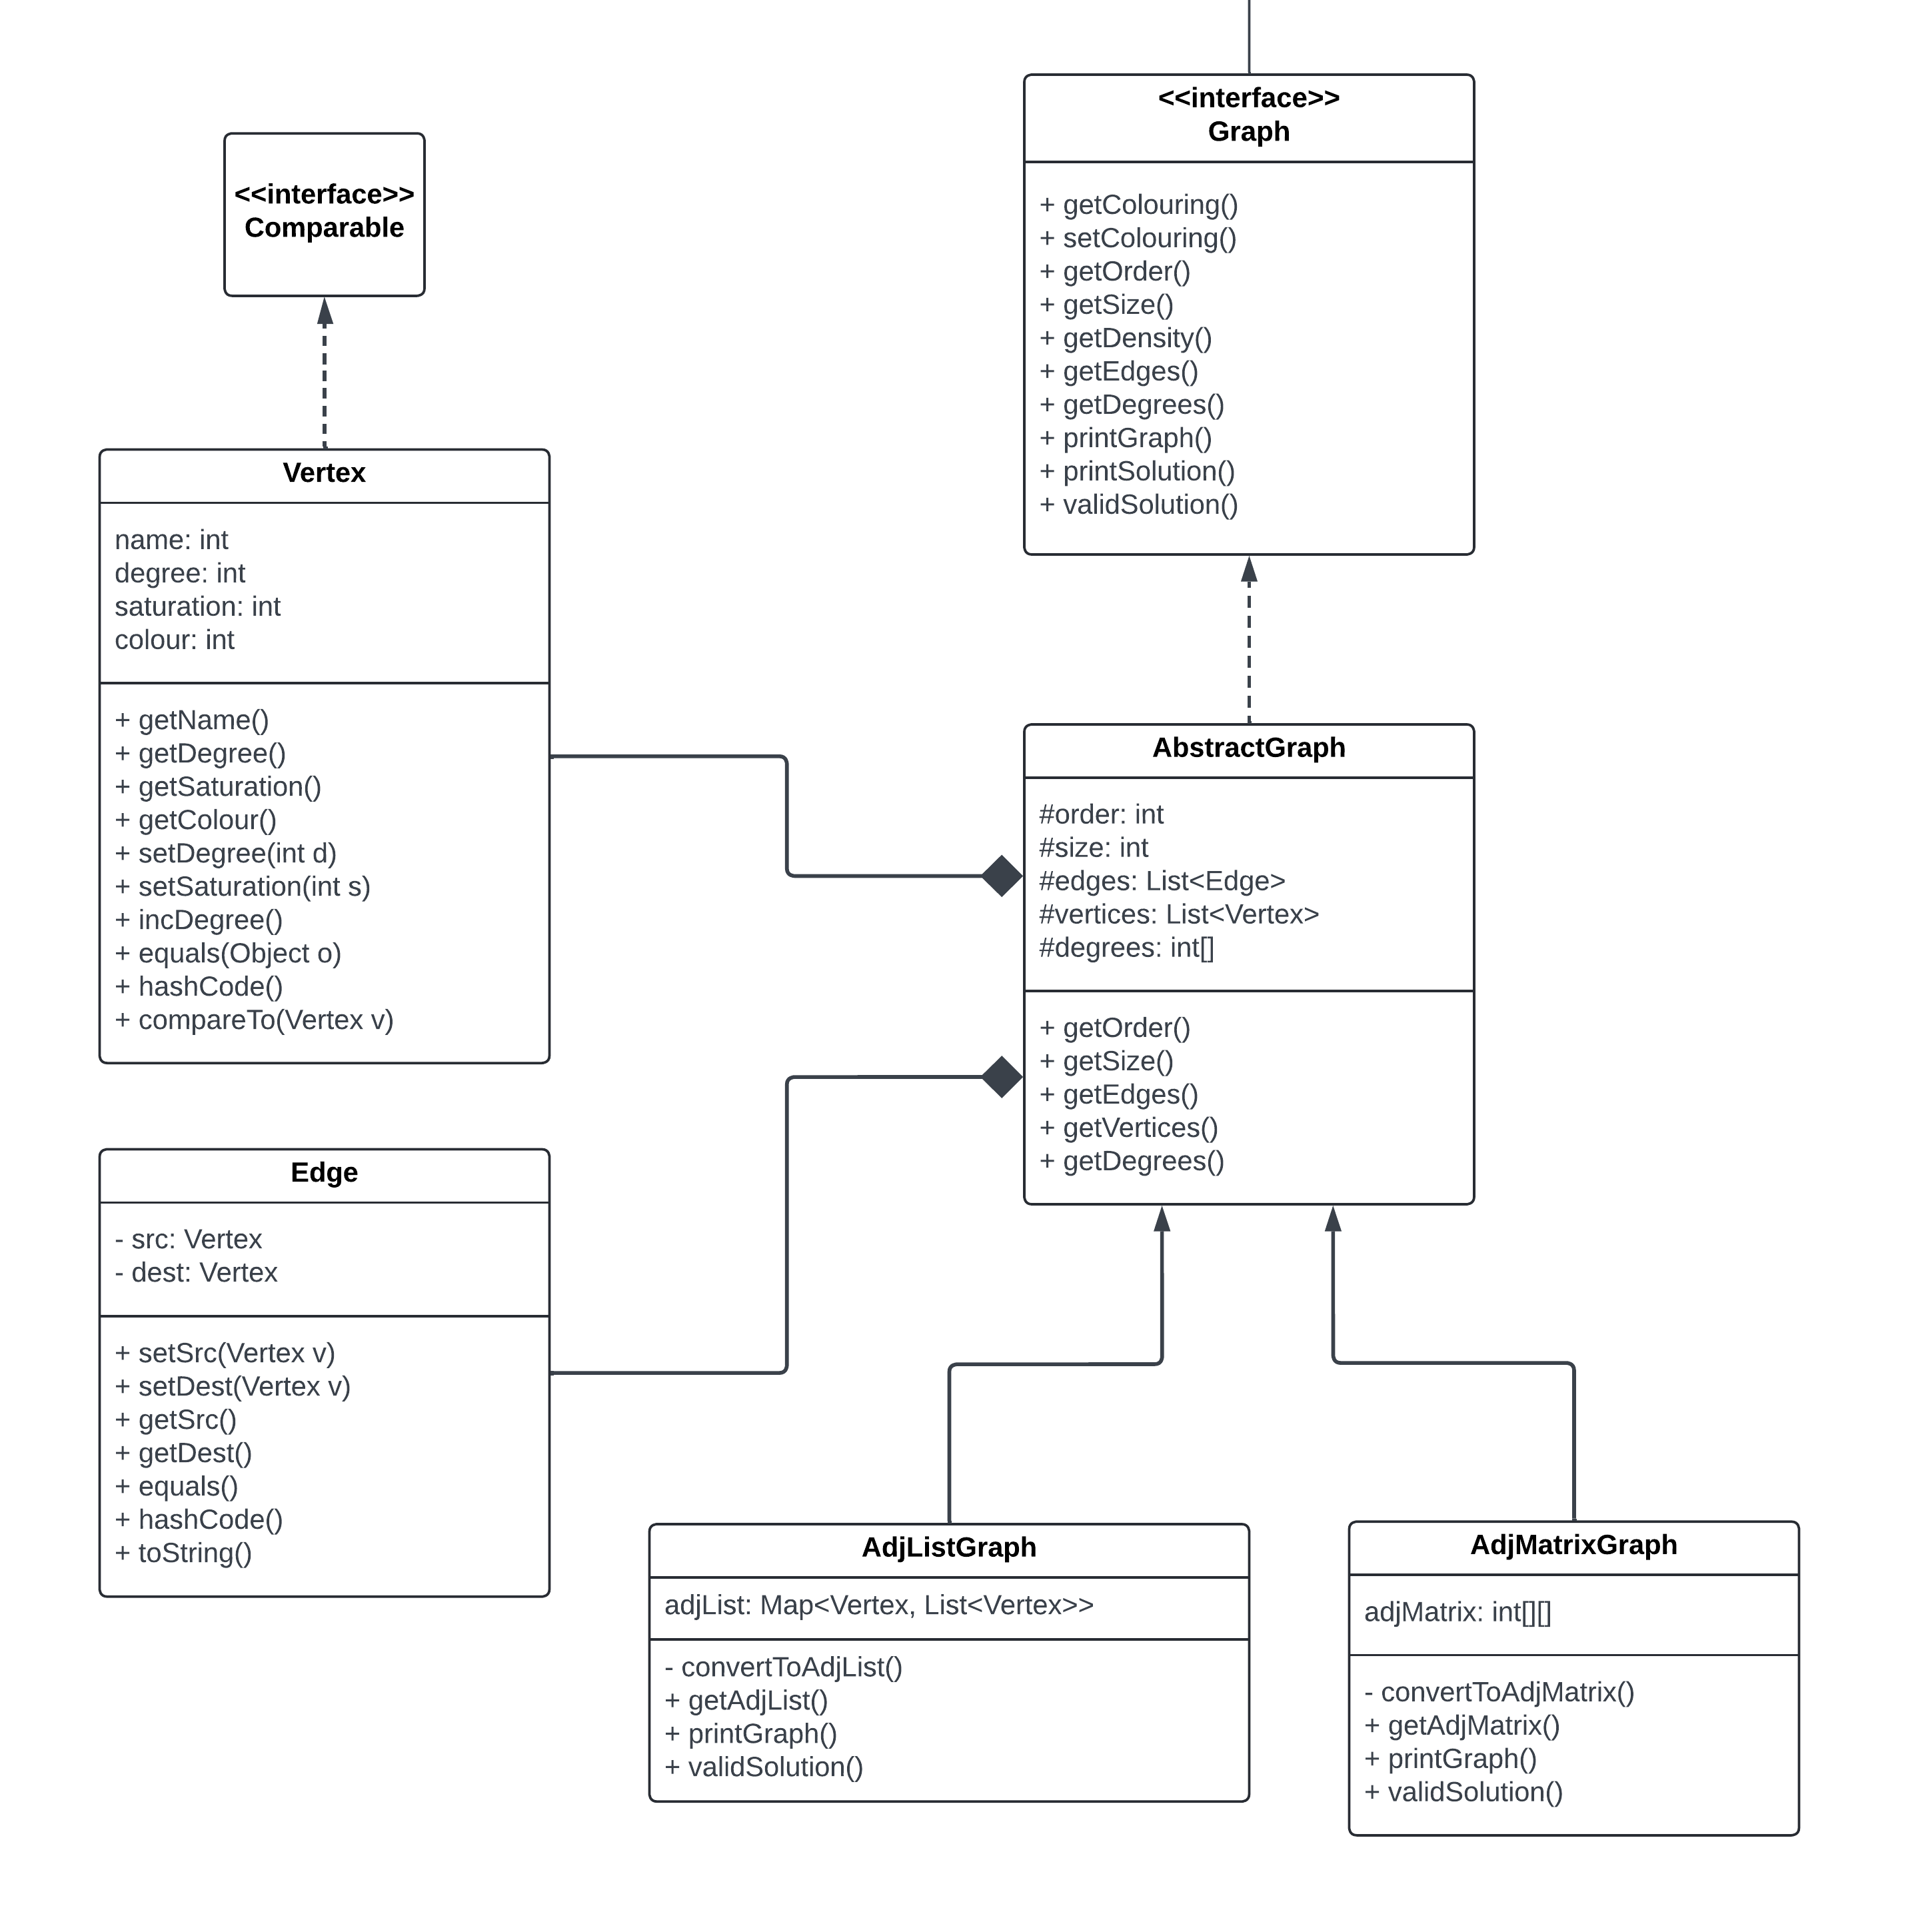
\includegraphics[width=0.9\linewidth]{Components/GraphHierarchy.png}
    \caption{UML class diagram showing the classes that make up the Graph Hierarchy}
    \label{fig:GraphHierarchy}
\end{figure}

The algorithms themselves (shown in Figure \ref{fig:GraphColouringHierarchy}) have been designed in a way to abstract anyone making use of them from their implementation. Each algorithm will have two methods that can be used to colour an input graph and to retrieve the number of checks or operations an algorithm must do to find a solution. A colouring will return a solution in the form of a Map that maps an integer colour to a set of vertices that make up the colour set. 
\\\\

\begin{figure}[H]
    \centering
    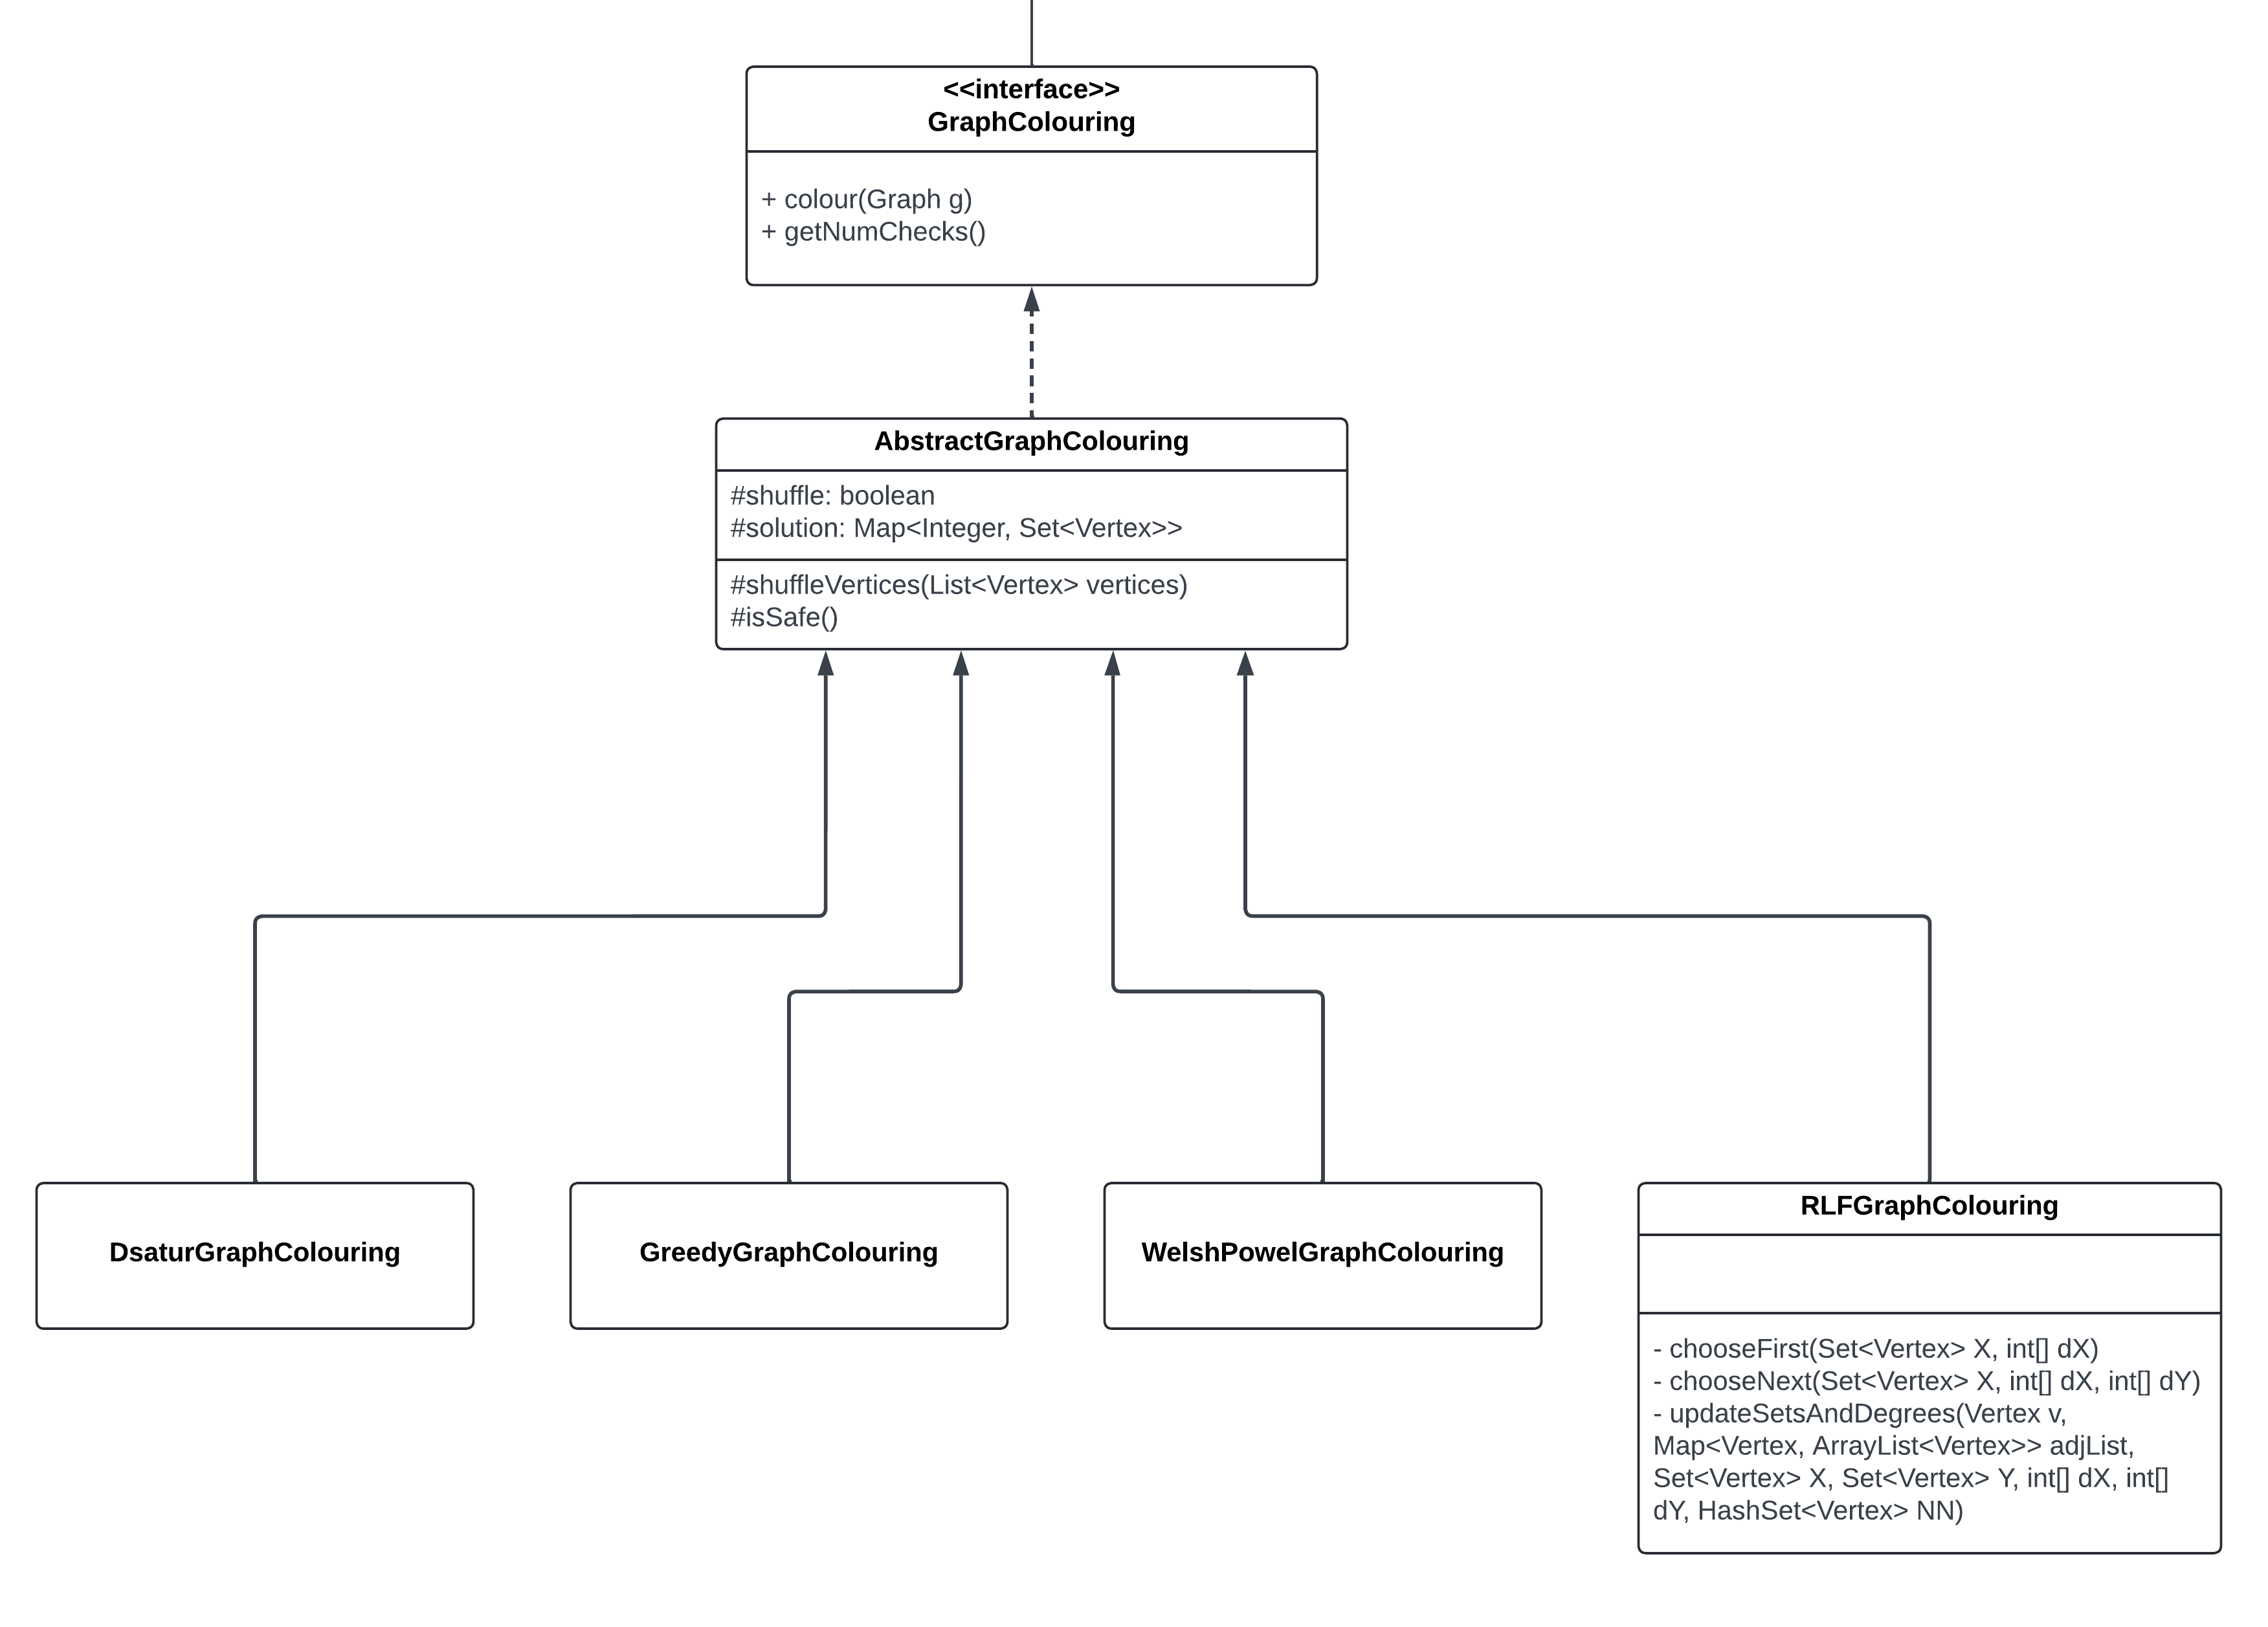
\includegraphics[width=0.9\linewidth]{Components/ColouringHierarchy.png}
    \caption{UML class diagram showing the classes that make up the Graph Colouring Algorithms Hierarchy}
    \label{fig:GraphColouringHierarchy}
\end{figure}

\begin{figure}[H]
    \centering
    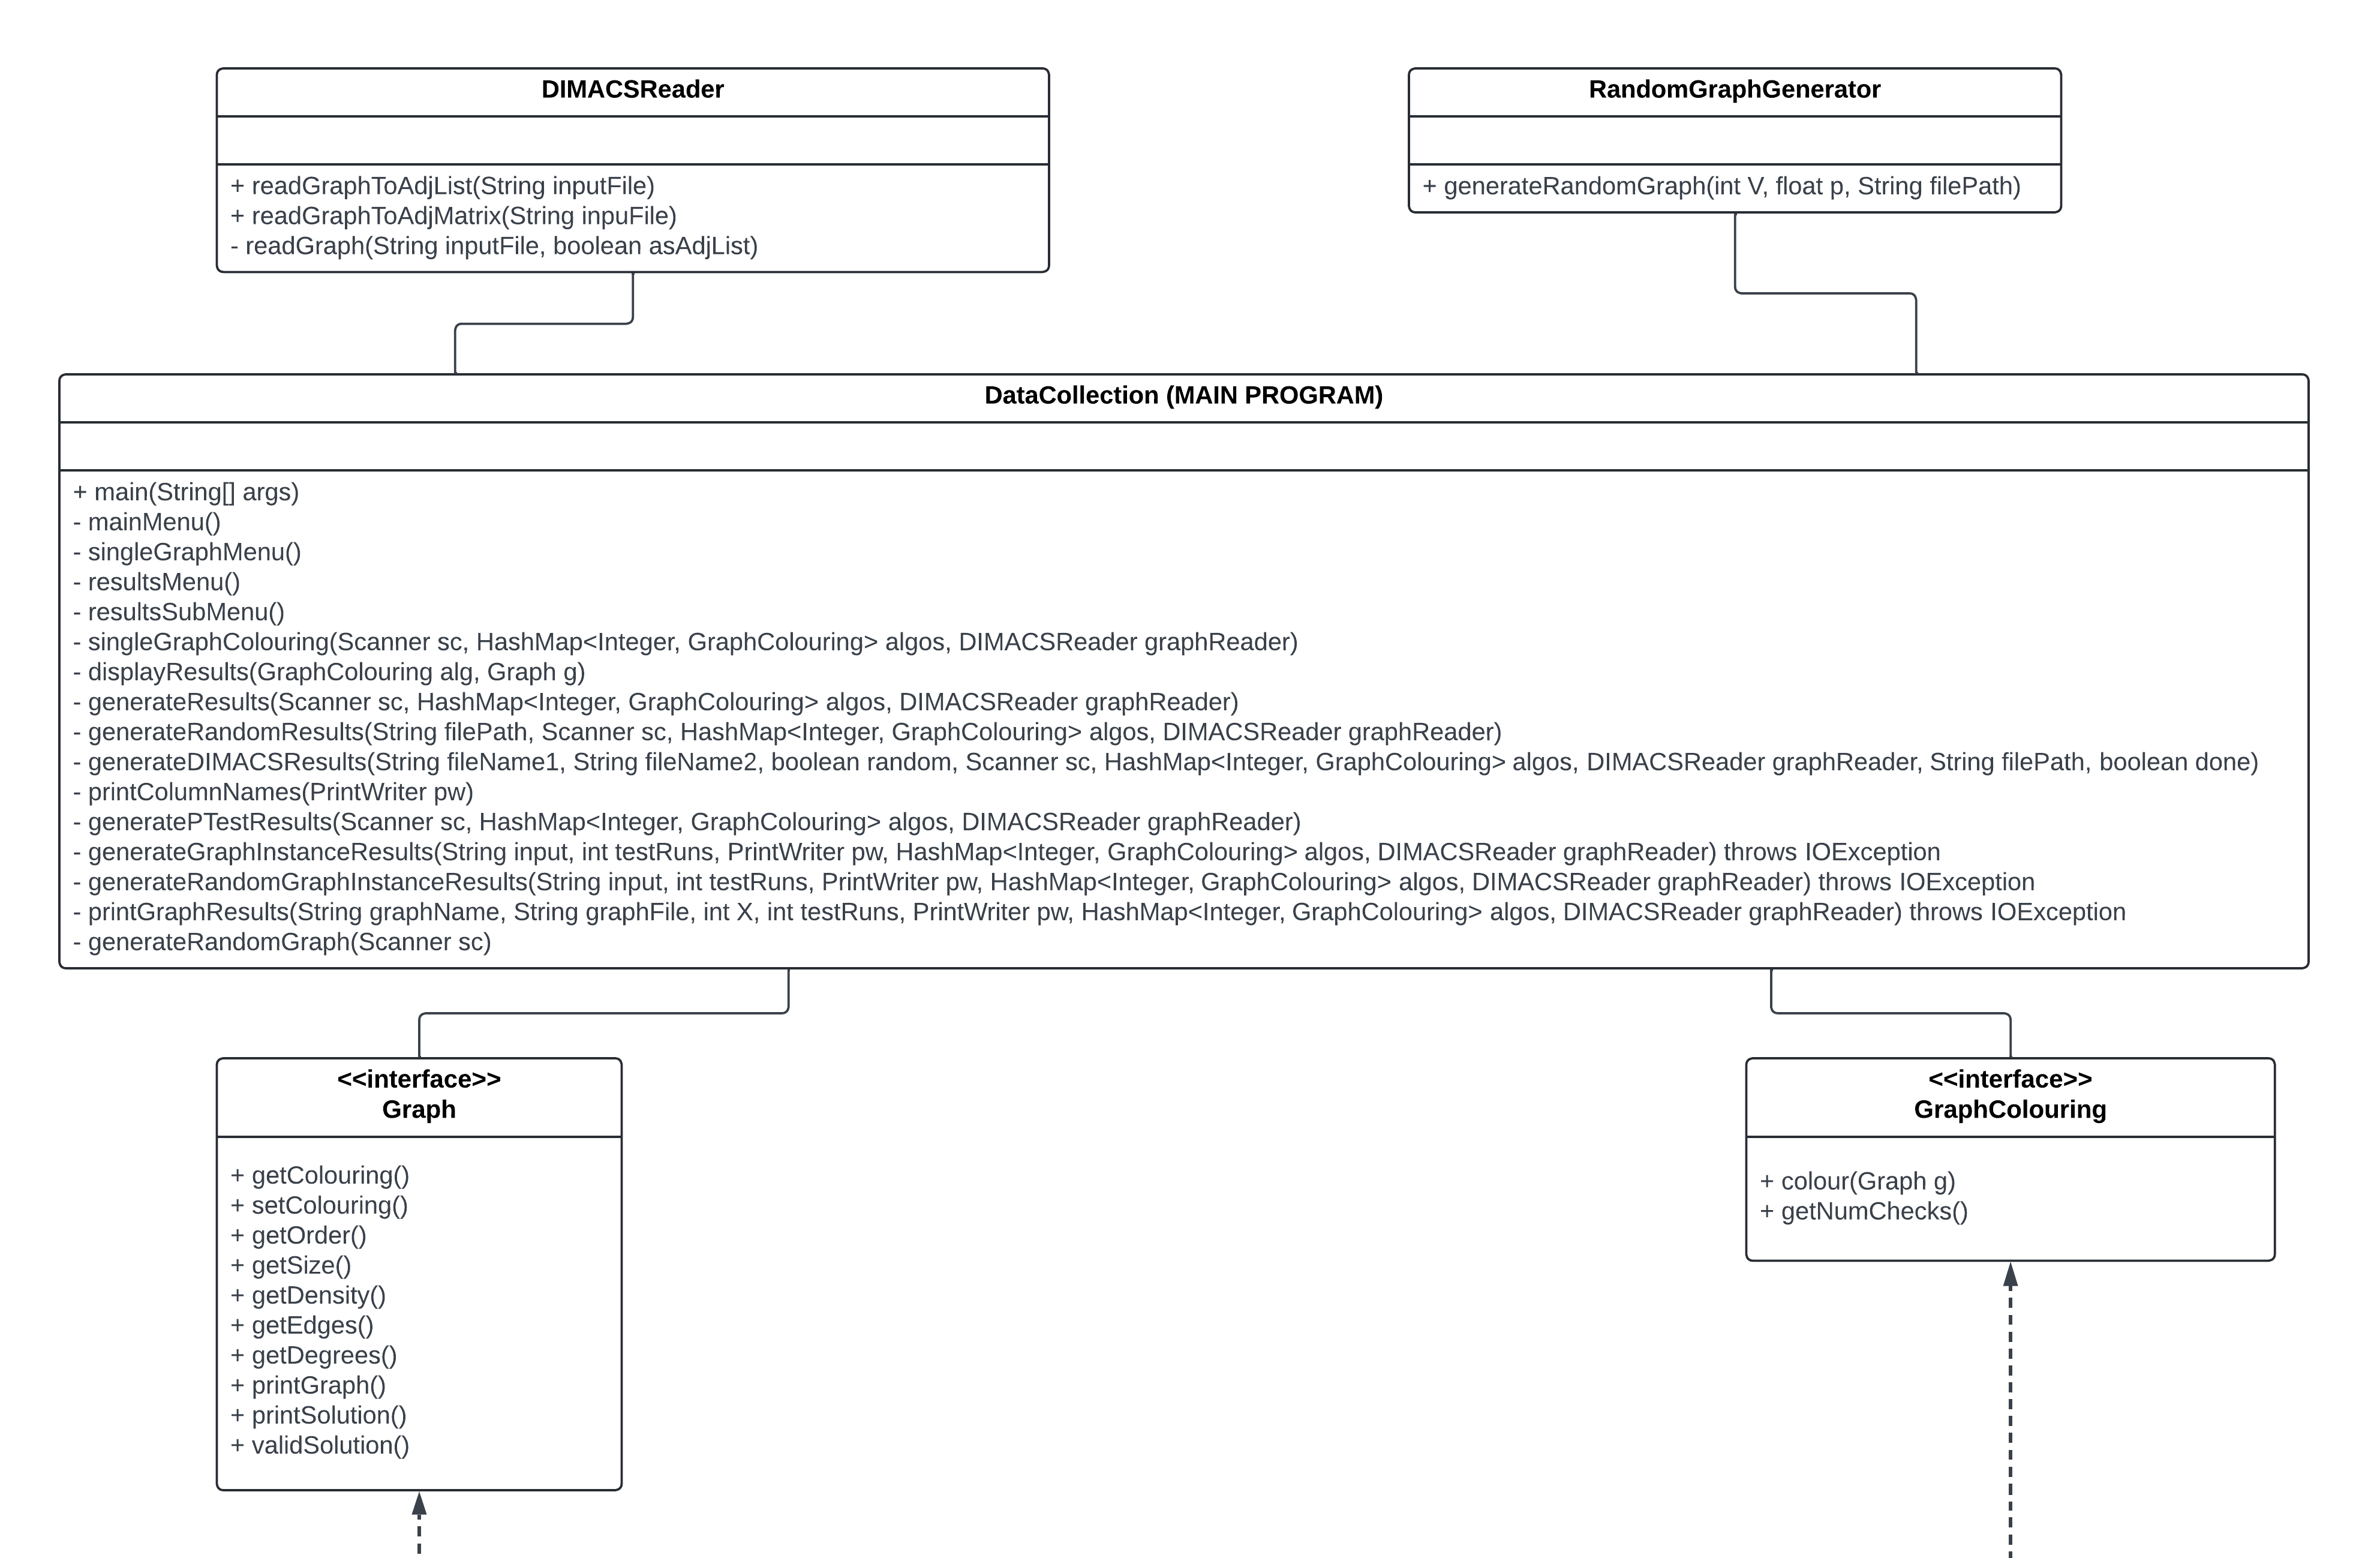
\includegraphics[width=0.9\linewidth]{Components/MainProgram.png}
    \caption{UML class diagram showing the classes that make up the Main Program}
    \label{fig:MainProgram}
\end{figure}

Finally, Figure \ref{fig:MainProgram} shows the design of the main program, along with the classes it uses to function. The main program is designed to provide a simple terminal UI that will satisfy the requirements set out in section 3.1. This includes a DIMACSReader class that allows for graphs to be read in from files. It also includes a RandomGraphGenerator class that has the ability to generate a random $G(n, p)$ graph and print it to an output file. 

\subsection{Implementation}
The following section provides some details into the implementation of the graph colouring software. The tasks for implementation were split into segments to mimic the idea of sprints in agile development. Each section typically follows chronologically from how they were implemented. As might be expected with agile development, however, each section was not necessarily developed independent from another. 

\subsubsection{Reading and Storing Graphs}
The first task was to find a way to read in DIMACS format graphs from an external file and then store them in a way that would be useful for running the algorithms on. The standardisation of the DIMACS format makes the reading of these files quite simple as a single method is required and it will never fail providing the file is in the correct format. The format is as follows:
\begin{verbatim}
    c lines beginning with c are a comment line 
    c describing the graph or any extra details
    c
    p edge Order Size
    e 1 2
    e 1 4
    .
    .
    .
\end{verbatim}
The lines  beginning with "c" are comment lines that provide the graph name and can include extra information about the graph such as density, chromatic number etc. For the purposes of reading in the graph the comment lines are generally ignored. The line starting "p" is where the reading in starts, this line provides the total number of vertices of the graph (Order) and the total number of edges (Size). This provides some useful information in order to set up the data-structures to store the information that is about to be read. The lines beginning with "e" are the graph itself. They are referred to as edge lines with the first number being one vertex and the second being another vertex. If two numbers share an edge line then they also share an edge. 
\\\\
In implementing the method to read the graph, considerations were made about disconnected vertices (i.e vertices that did not appear on an edge line), and handling bad input (such as incorrect file input, or incorrect file format). Important information that may be useful was also extracted from the reading process. This includes information about the degrees of each vertex, and the maximal degree vertex. 
\\\\
 In conjunction with building the method for reading in graphs, a storage hierarchy for the graphs themselves was being constructed. The hierarchy implemented closely follows the design set out in Figure \ref{fig:GraphHierarchy}. Each graph that is read in can be stored as either an Adjacency List graph or an Adjacency Matrix graph. A Graph is made up of Vertex and Edge objects. The reason for making a class of Vertex was to take advantage of the Comparable interface that Java provides. This allowed for ordering of Vertex objects within the constraints of some of the algorithms (i.e. in order of saturation for DSATUR or in order of degree for WELSH-POWELL). Similarly making a class of Edge allowed for checking if two edges are the same. This is necessary as graph colouring is done on directionless graphs so an edge $e\{1 \rightarrow 2\} \equiv e\{2 \rightarrow 1\}$. 
 
\subsubsection{Algorithms}
The algorithms themselves were the next part to be implemented. The following presents and explains the implementation, in pseudocode format, of the algorithms used in this project. Due to similarities between the GREEDY, SHUFFLED GREEDY and WELSH-POWELL1 algorithms, only the GREEDY pseudocode will be included. However, the slight variations between the three in implementation will be explained. 

\begin{figure}[H]
    \centering
        \begin{algorithm}[H]
        \DontPrintSemicolon
        \SetKwInOut{Input}{input}\SetKwInOut{Output}{output}
        
        \Input{A Graph G where $V$ is the set of Vertices and $A$ is the adjacency list}
        \Output{$S$ A Map of Coloured Vertex Sets}
        \BlankLine

        $S \leftarrow \emptyset$ \;
        \For{$v \in V$ \KwTo $|V|$}{
            $N \leftarrow A_{v}$ \;
            \For{$c \leftarrow 0$ \KwTo $|V|$}{
                \If{$!S_{c}$}{$S_{c} \leftarrow \emptyset$}
                Safe $\leftarrow True$ \;
                \For{$n \in N$ \KwTo $|N|$}{
                    \If{$n_{c} == c$}{
                        Safe $\leftarrow False$ \;
                        break \;
                    }
                }
                \If{Safe}{
                    $v_{c} \leftarrow c$ \;
                    $S_{c} \leftarrow S_{c} \cup \{v\}$
                }
            }
        }
        
        \caption{GREEDY}
        \end{algorithm}
    \caption{Pseudocode for the implementation of the GREEDY algorithm}
    \label{fig:GreedyImpPseudo}
\end{figure}

Figure \ref{fig:GreedyImpPseudo} shows the pseudocode of the implementation used for the GREEDY algorithm. Line 1 sets up $S$ (the solution to be returned) as an empty map, the map operates by mapping a colour, in this case an integer from $0 \rightarrow k$, to a set of vertices. The colour set created is denoted by $S_{c}$. Line 2 begins the loop iterating through every vertex of the graph. In the case of the GREEDY algorithm it will do this in order from $v_{1} \rightarrow v_{i}$ where $i$ is the order of the graph. Line 3 retrieves all the neighbours of the vertex $v$ from the adjacency list and assigns it to the variable $N$. On line 4 it starts looping through the colours in order to find a suitable colour, remembering that the GREEDY approach is to take the first feasible colour it can find. Lines 5-7 is a simple check that makes sure that if the colour has not been reached before then a new set will be constructed within the solution map. The main power of the GREEDY algorithm in providing correct solutions comes in lines 8-14. It loops through all the neighbours of $v$ and checks if the colour they have been assigned is the same as the current colour it is trying to assign to $v$. If it reaches any conflict it breaks out of the loop and moves on to the next colour. However, if it finds no conflicts it assigns $v$ with that colour and puts $v$ in the colour set $S_{c}$ as shown in lines 15-18. It then repeats the process for the the rest of the vertices until they have all been assigned a colour. 
\\\\
As mentioned previously the pseudocode for SHUFFLED GREEDY and WELSH-POWELL1 have not been included as they both build of the GREEDY method but simply change the ordering of the vertices. Therefore there is just one additional step required which is changing the order in which vertices are coloured. As mentioned in section 2 the SHUFFLED GREEDY method shuffles the vertices into a pseudo-random order using a random number generator to decide how to shuffle them. The WELSH-POWELL1 method sorts the vertices in order of their degree.

\begin{figure}[H]
    \centering
        \begin{algorithm}[H]
        \DontPrintSemicolon
        \SetKwInOut{Input}{input}\SetKwInOut{Output}{output}
        \SetKw{and}{and}
        
        \Input{A Graph G where $V$ is the Queue of Vertices (sorted by degree) and $A$ is the adjacency list}
        \Output{$S$ A Map of Coloured Vertex Sets}
        \BlankLine

        $S, X \leftarrow \emptyset$ \;
        $c \leftarrow 0$ \;
        \While{$|X| \neq |G|$}{
            $S_{c} \leftarrow \emptyset$ \;
            $v \leftarrow V_{first}$ \;
            $v_{c} \leftarrow c$ \;
            $S_{c} \leftarrow S_{c} \cup \{v\} $, $ X \leftarrow X \cup \{v\}$ \;
            \tcc{build set of non-neighbouring vertices of $v$}
            $N \leftarrow A_{v}, notN \leftarrow \emptyset$ \;
            \For{$u \in V$ \KwTo $|V|$}{
                \If{$u \notin N$}{
                    $notN \leftarrow N \cup \{u\}$
                }
            }
            \ForEach{$u \in notN$}{
                \tcc{same safety check as in GREEDY}
                \If{$u_{c} < 0$ \and Safe}{
                    $u_{c} \leftarrow c$ \;
                     $S_{c} \leftarrow S_{c} \cup \{u\} $, $ X \leftarrow X \cup \{u\}$ \;
                } 
            }
            $S \leftarrow S \cup S_{c}$ \;
            $c \leftarrow c + 1$
        }
       
        
        \caption{WELSH-POWELL2}
        \end{algorithm}
    \caption{Pseudocode for the implementation of the WELSH-POWELL2 algorithm}
    \label{fig:WP2ImpPseudo}
\end{figure}

Figure \ref{fig:WP2ImpPseudo} shows the implementation of the second variation of the WELSH-POWELL algorithm. The algorithm starts off by instantiating (initially empty) the map of $S$ (solution) and a set $X$ to keep track of which vertices have been coloured. On line 2 it starts by assigning the first colour to be constructed as 0, and line 3 begins the while loop within which each colour set will be constructed. Lines 4-7 show the process of selecting and colouring the first vertex of the colour set being constructed $S_{c}$. It selects the first vertex by taking the first vertex from $V$ (the queue of vertices). The first vertex being the one with the highest degree that has not yet been coloured. It then assigns the current colour to $v$ and adds it to the colour set $S_{c}$ and the set $X$ of coloured vertices. Lines 9-14 build a set containing all the vertices that are not a neighbour of $v$ meaning it may be eligible for the current colour set. Lines 15-21 go through the process of adding these candidate vertices to the colour set if: the candidate has not been coloured; and it is safe to do so (using the same safety check as in GREEDY). Finally, lines 22-23 show the constructed colour set being put in $S$ and increments to the next colour set to be constructed. The algorithm terminates when all the vertices have been assigned to a colour set. 

\begin{figure}[H]
    \centering
        \begin{algorithm}[H]
        \DontPrintSemicolon
        \SetKwInOut{Input}{input}\SetKwInOut{Output}{output}
        \SetKwFunction{uS}{updateSaturation}
        
        \Input{A Graph G where $V$ is the set of Vertices and $A$ is the adjacency list}
        \Output{$S$ A Map of Coloured Vertex Sets}
        \BlankLine

        $S \leftarrow \emptyset$,
        $Q \leftarrow V$ \;
        \While{$Q \neq \emptyset$}{
            $v \leftarrow Q_{first}$ \;
            $c \leftarrow 0$ \;
            \For{$c$ \KwTo $|V|$}{
                \If{$!S_{c}$}{$S_{c} \leftarrow \emptyset$}
                \If{Safe}{
                    $v_{c} \leftarrow c$,
                    $S_{c} \leftarrow S_{c} \cup \{v\} $
                }
            }
            \tcc{Remove $v$ from the graph and update the degrees and saturation of its neighbouring vertices in the induced subgraph}
            $N \leftarrow A_{v}$ \;
            \ForEach{$n \in N$}{
                \If{$n_{c} < 0$}{
                    $n_{d} \leftarrow n_{d} - 1$ \;
                    \uS{$n$} \;
                }
            }
        }
    
        \caption{DSATUR}
        \end{algorithm}
    \caption{Pseudocode for the implementation of the DSATUR algorithm}
    \label{fig:DSATURImpPseudo}
\end{figure}

Figure \ref{fig:DSATURImpPseudo} shows the implementation of the DSATUR algorithm. The algorithm starts off by using a Priority Queue denoted by $Q$ which works similarly to a heap data-structure. A heap is a type of tree data-structure where each parent node is either greater than (making a max heap) or less than (making a min heap) its child node. In this case $Q$ uses two constraints to order the vertices. The first and most important constraint is the saturation of the vertices. As established in section 2, saturation is the number of different colours that neighbour a vertex. The second constraint is the degree of the vertex. In short, vertices with the highest saturation are placed at the front of $Q$. If multiple vertices have the same saturation then the vertex with the highest degree comes first. If vertices have the same saturation and the same degree then the choice is arbitrary, in this case the vertex with the lowest label is chosen. This method of ordering is where the main power of DSATUR comes from. It then assigns the minimum colour it can to each vertex $v$. Therefore, on line 3, the algorithm chooses the first vertex from $Q$ given the constraints just established, and removes it from $Q$. Lines 4-12 are almost identical to that of the GREEDY algorithm simply choosing the minimal safe colour to assign to the vertex $v$. Lines 14-20 are bookkeeping to ensure the saturation and degrees of each neighbouring vertex of $v$ is updated for the next iteration. The process then repeats for the next vertex until all vertices are coloured, in this case when $Q$ is empty. 

\begin{figure}[H]
    \centering
        \begin{algorithm}[H]
        \DontPrintSemicolon
        \SetKwInOut{Input}{input}\SetKwInOut{Output}{output}
        \SetKwFunction{uDAS}{updateSetsAndDegrees}
        
        \Input{A Graph G where $V$ is the set of Vertices and $A$ is the adjacency list}
        \Output{$S$ A Map of Coloured Vertex Sets}
        \BlankLine

        $S \leftarrow \emptyset$ \;
        $X \leftarrow V$, $Y \leftarrow \emptyset$ \;
        $c \leftarrow 0$ \;
        \While{$X \neq \emptyset$}{
            $S_{c} \leftarrow \emptyset$ \;
            $v \leftarrow X_{first}$ \;
            $v_{c} \leftarrow c$,
            $S_{c} \leftarrow S_{c} \cup \{v\}$ \;
            \uDAS{$v$, $X$, $Y$} \;
            \While{$X \neq \emptyset$}{
                $u \leftarrow X_{next}$ \;
                $u_{c} \leftarrow c$, 
                $S_{c} \leftarrow S_{c} \cup \{u\}$ \;
                \uDAS{$u$, $X$, $Y$}
            }
            $S \leftarrow S \cup S_{c}$ \;
            $X \leftarrow Y$ \;
            $Y \leftarrow \emptyset$ \;
            $c \leftarrow c + 1$
        }
    
        \caption{RLF}
        \end{algorithm}
    \caption{Pseudocode for the implementation of the RLF algorithm}
    \label{fig:RLFImpPseudo}
\end{figure}

Finally, the implementation of RLF is shown in Figure \ref{fig:RLFImpPseudo}. The algorithm sets out by introducing two distinct sets that will be used throughout the algorithm to keep track of the vertices. The set $X$ holds the vertices that are candidates (initially all vertices) to be included within $S_{c}$, the colour set being constructed. Whereas, $Y$ holds the vertices that are not eligible to be included within $S_{c}$ (initially empty). On lines 6-7 the first vertex $v$ is selected from the candidate vertices in $X$ based on the vertex with maximal degree (any ties make selection arbitrary, as in DSATUR the vertex is chosen based on smallest label). On line 8 there is a call to a method that updates $X$ and $Y$ based on the vertex $v$ that is being coloured. All the neighbours of $v$ are placed in $Y$ as they can no longer be considered for $S_{c}$. The heuristics for the next vertex $u$ to be coloured (as established in section 2) are determined by the vertex with the most neighbours in $Y$. This process, shown on lines 9-13, is repeated until there are no candidates left in $X$. The colour set $S_{c}$ is then stored in $S$. All the vertices in $Y$ are moved over to $X$, and $Y$ is emptied. The process then starts over again constructing the next colour set until all the vertices of the graph have been coloured.  

\subsubsection{Random Graph Generator}

The next thing to be implemented was a method to generate random $G(n,p)$ graphs to test the algorithms on. This was made simple using  Java's inbuilt Random class. The method requires an input value of $n$ (being the total number of nodes of the graph being generated), and also a value for $p$ (being the probability that two vertices will share an edge). After that the method simply loops through all the possible edges of the graph and uses the random generator to determine if an edge will be created or not. An edge is created if the value that is generated by Random is smaller than $p$. The resulting graph is then printed to an output file in DIMACS format, along with some useful information, in the form:
\begin{verbatim}
    c File: {graph_name}
    c 
    c This is a randomly generated graph G(n, p) where: 
    c n (num vertices): {n_input}
    c p (edge probability): {p_input}
    c 
    c Graph Properties: 
    c Order: {n_input}
    c Size: ...
    c Density: ...
    c Maximum Degree: ...
    c Minimum Degree: ...
    c Average Degree: ...
    c 
    p edge Order Size
    e 1 5
    e 1 9
    .
    .
    .
\end{verbatim}

This allows for multiple $G(n,p)$ graphs to be generated and means that a user can utilise and reflect back on the useful information provided regarding the graphs topology. 

\subsubsection{Main Program}
The final stage of implementation was to create a simple terminal based UI in order to generate the results required to achieve the project aims. Figure \ref{fig:MainMenu} shows the main menu of the terminal program. This was implemented to satisfy the functional and non-functional requirements set out in section 3.1 Table \ref{tab:FuncReqs} and Table \ref{tab:NonFuncReqs} respectively. Option 1 allows users to test the algorithms on a single test instance, thus satisfying FR1. Option 2 allows users to generate results on various DIMACS test instances, satisfying FR9. Option 3 allows for the generation of results testing the algorithms on $G(n, p)$ graphs, satisfying FR10. Option 4 allows for the generation of a new $G(n, p)$ graph, satisfying FR11. Finally, option 5 allows the user to quit the program, satisfying FR13 and NFR6. 
\begin{figure}[H]
    \centering
    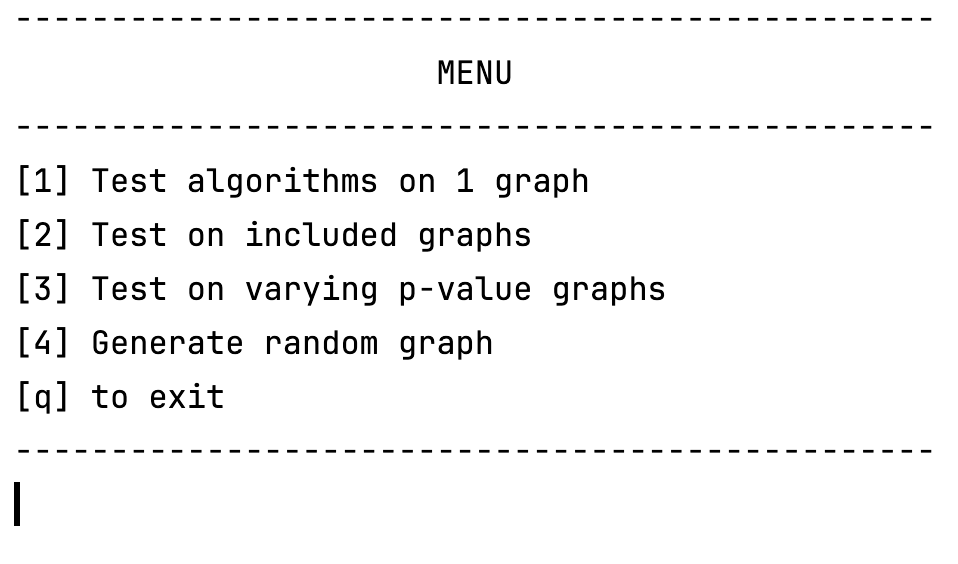
\includegraphics[width=0.5\linewidth]{Components/MainMenu.png}
    \caption{Main Menu of the terminal program}
    \label{fig:MainMenu}
\end{figure}

After selecting option 1 on Figure \ref{fig:MainMenu} the program prompts you to input a graph file path and directs you to the algorithm selection menu as shown in Figure \ref{fig:AlgSelect}. The user may then select which algorithm (or input 6 to select all) to use and the program will print the results to the terminal. If the user provides any incorrect input, they will be directed to start the process again. This satisfies FR2-FR8 and NFR2. 

\begin{figure}[H]
    \centering
    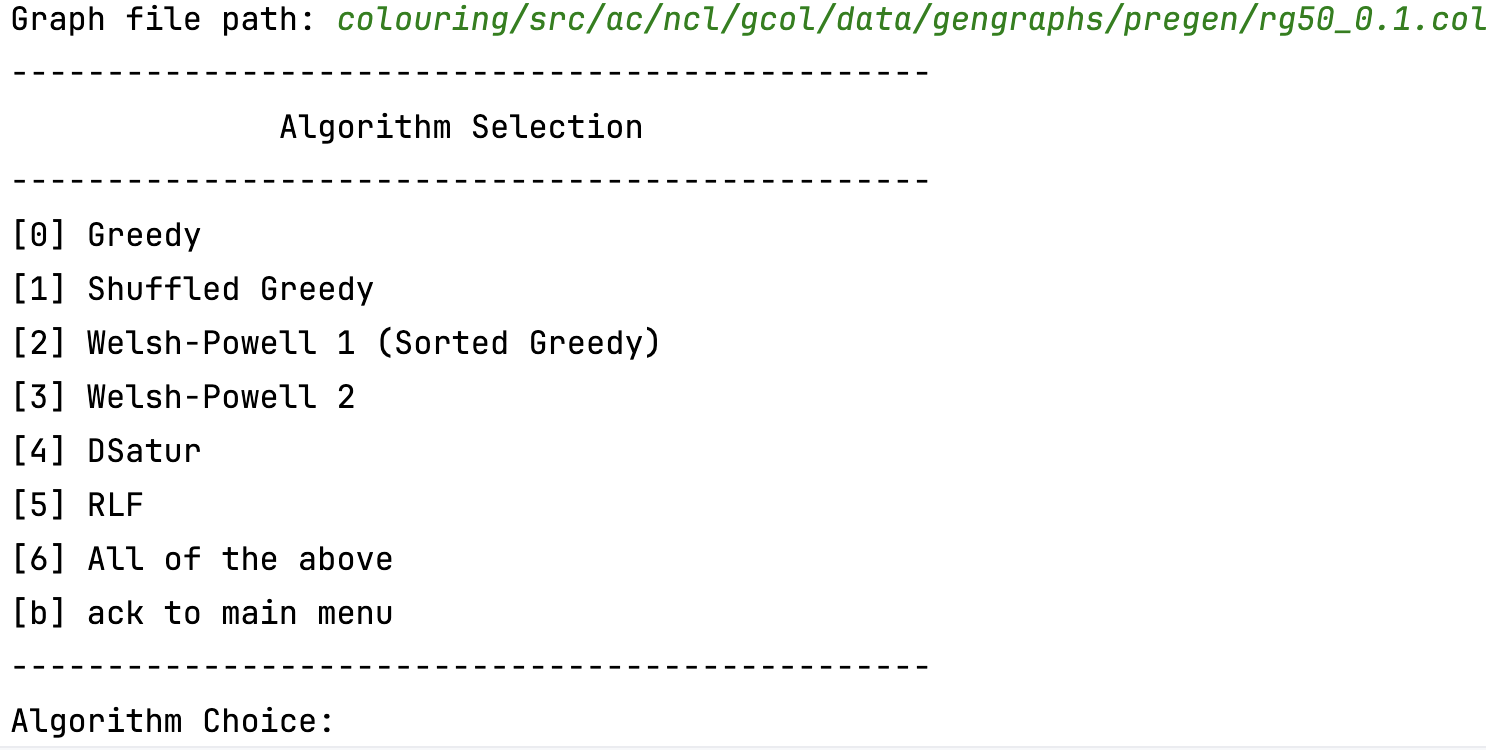
\includegraphics[width=0.5\linewidth]{Components/AlgorithmSelection.png}
    \caption{Algorithm selection menu for colouring a single graph}
    \label{fig:AlgSelect}
\end{figure}

After selecting option 2 from Figure \ref{fig:MainMenu} the user will be directed to choose the type of graph instance they wish to generate results for, as shown in Figure \ref{fig:GtypeSelect}. The program will then run the algorithms on the desired test instances and output the results to a CSV file. The results will include the number of colours $k$ each algorithm uses, the number of operations each algorithm performs, and the time (in nanoseconds) it takes for an algorithm to find the solution. If the user provides any incorrect input, they will be directed to start the process again. This satisfies NFR3. 
\begin{figure}[H]
    \centering
    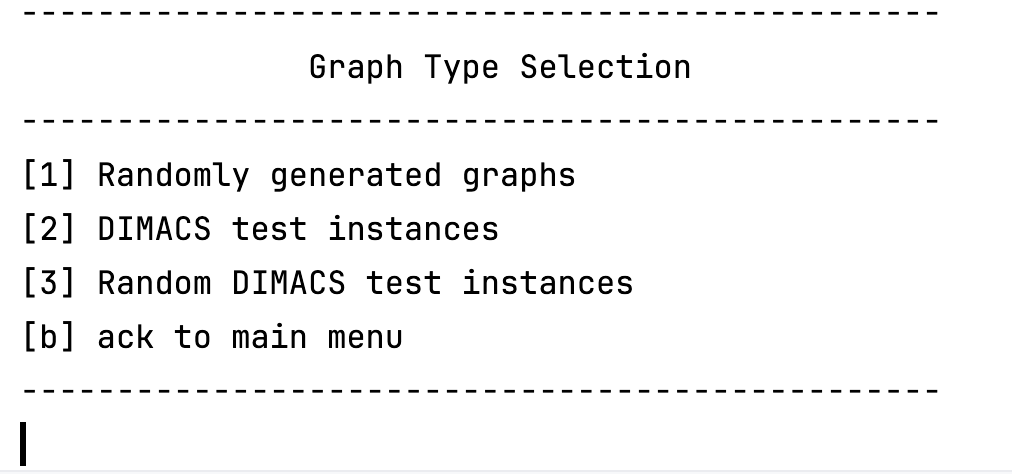
\includegraphics[width=0.5\linewidth]{Components/GraphTestSelection.png}
    \caption{Graph type selection menu for testing algorithms and generating results}
    \label{fig:GtypeSelect}
\end{figure}
After selecting option 3 from Figure \ref{fig:MainMenu} the user will be directed to answer questions regarding the types of $G(n, p)$ graph they would like to test on. The first question the user will be asked is the number of variations of $G(n, p)$ to generate per $p$-value. Then, users will be asked to input the desired $p$-values to test on in a comma separated list. Finally, users will be asked to input a value for $n$ (the number of nodes). The program will then generate the desired results and output these to a CSV file. The results will be in the same format as those generated from option 2. If the user provides any incorrect input, they will be directed to start the process again. This satisfies NFR4.
\begin{figure}[H]
    \centering
    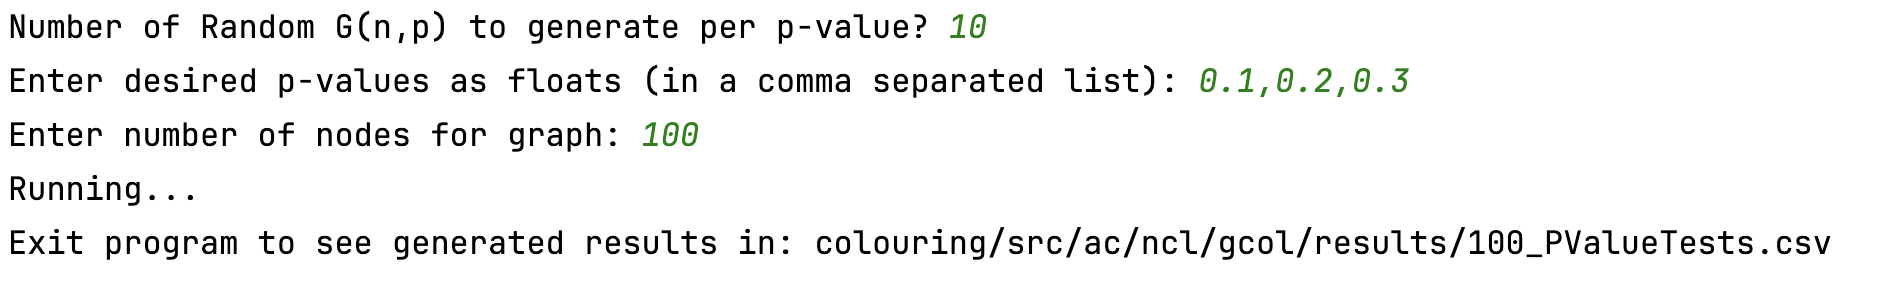
\includegraphics[width=0.7\linewidth]{Components/RunningTests.png}
    \caption{Running algorithms and generating results for $G(n, p)$ graphs}
    \label{fig:enter-label}
\end{figure}
After selecting option 4 from Figure \ref{fig:MainMenu} the user is prompted to input a value for $n$ and a value for $p$. The graph is then generated and outputted to a file in DIMACS format. This satisfies NFR5.

\subsection{Testing}
Due to the time constraints of this project, formal unit testing was not feasible. Instead, several checks were performed whilst the program was being implemented. Firstly, whilst building the graph reader it was ensured that all information stored within the graph objects matched the information of the input file. For example, it was ensured that the density, maximal degree, and average degree of the vertices were the same in both. Secondly, whilst building the graph storage, small graph instances were visually inspected (by printing to the terminal) to ensure they matched the input file. For the algorithms themselves several testing methods were adopted. In some cases (specifically in small test instances) solutions were generated by hand to ensure that the solution generated by the program was accurate. In other cases, the result was checked against known results for the particular algorithm to ensure accuracy. A method was created to ensure that all solutions generated were correct solutions (i.e. there were no colouring conflicts). With regard to the random graph generator, it was ensured that the $p$-value chosen and the density of the graph were similar (as these are linked). Finally, with regards to the main program, user testing was performed iteratively during the development process to ensure that features worked as expected and were in accordance with the requirements.
\\\\
In terms of testing the algorithms performance against the metrics established in the aims of this project, the decision was made to test $G(n, p)$ graphs with varying $n$ and $p$-values and test DIMACS instances with known chromatic numbers. As $p$-values and density are linked, increasing $p$ will increase the density of the graph. Therefore, decision to test $p$-values 0.1, 0.2, 0.3, 0.4, 0.5, 0.6, 0.7, 0.8, and 0.9 was made because it will allow the author to measure the algorithms performance on a variety of graphs from those that are sparse to those that are extremely dense. This will allow the author to see the effectiveness and efficiency of the algorithm as the graph becomes denser. Likewise, altering $n$ values will have a similar effect. Therefore, the decision was made to test $n$ values of 50, 100, 150, 300, 500, 750, 1000, and 1500 as this will provide sufficient difference in number of nodes to see change in algorithm effectiveness and efficiency, whilst being small enough to be manageable within the time constraints. 20 test runs were performed per value of $p$ to provide averages for the number of colours used, number of operations performed, and time taken.
\\\\
Testing only DIMACS instances with known chromatic numbers was also performed, as this provides a metric to determine the effectiveness of the algorithms by comparing the difference between the number of colours used and the chromatic number of the graph. A list of the graphs can be seen in Table \ref{tab:DIMACSResults} (section 4.3). These graphs were taken from the second DIMACS implementation challenge \cite{DIMACSChallenge2}. Leighton's random graphs with known chromatic numbers (shown in Table \ref{tab:LeightonGraphResults}, section 4.4), were also tested to provide a similar metric to determine the effectiveness of the algorithms. The format of this table is based on the table presented by Leighton in his seminal formulation of the RLF algorithm \cite{Leighton1979AGC}. Similar to tests on $G(n, p)$ graphs, 20 test runs were performed per value of $p$ to provide averages for the number of colours used.

\section{Results}
For the results section the decision was made to only include the first variation of the WELSH-POWELL algorithm. This is because both the WELSH-POWELL1 and WELSH-POWELL2 algorithms produced the same results in terms of colouring, only WELSH-POWELL2 was less efficient. Therefore, it seems unlikley for there to be a context in which WELSH-POWELL2 would be a more optimal choice than WELSH-POWELL1. 
\\\\
This section will firstly look at the efficacy of algorithms in colouring $G(n, p)$ graphs by measuring the number of colours they require to find solutions while varying values of $n$ and $p$. This section will then look out how efficient the algorithms are at finding solutions for $G(n, p)$ graphs. Finally, this section will look at DIMACS test instances taken from the implementation challenge \cite{DIMACSChallenge2}. This will include test instances with known chromatic numbers as well as Leighton graphs (also part of DIMACS test instances) that are randomly generated but have a known chromatic number \cite{Leighton1979AGC}. Efficacy will be measured in these cases by the difference in the number of colours used by the algorithm and the chromatic number of the test instance. 
%%%%%%%%%%%%%%%%%%%%%%%%%%%%%%%%%% SECTION 4.1 %%%%%%%%%%%%%%%%%%%%%%%%%%%%%%%%%
\subsection{Colouring randomly generated  $G(n, p)$ graphs}


The first section of testing was performed on randomly generated $G(n, p)$ graphs where $n$ is the number of vertices, and $p$ is the edge probability. The first few results show the efficacy of the algorithms as the value of $p$ increases for particular values of $n$. Each point is taken from the mean of generating of 20 $G(n,p)$ graphs and running each algorithm on them once. Due to the similarity in trends for each graph of $n$ it was decided to only show graphs for values of $n$ at 50, 500, 1500. However all the data gathered to generate these results can be found in Appendix A.1. 
\\\\
Figure \ref{fig:V50p} shows that, for a small graph, DSATUR proves slightly more efficacious than RLF over most values of $p$. It is particularly more effective when the graph is sparse (i.e. $p$ is small). This may be due to the nature of the RLF algorithm in building up colour sets in contrast to DSATUR that colours the optimal vertex per iteration. This may mean that, when the graph has fewer constrained nodes (i.e. the graph is sparse and there are fewer nodes overall), the approach of DSATUR to take the locally optimal decision means that it can assign the later nodes to smaller colour sets. On the other hand, RLF builds up colour sets one by one and therefore may assign vertices, that could have been assigned to earlier colour sets, later than necessary. As can be seen in Figure \ref{fig:V50p}, the difference is rather minimal i.e. differing in one or two colour sets per value $p$. In the middle, as was expected, is the WELSH-POWELL algorithm which provides an extra ordering technique that means the more constrained vertices (i.e. those with highest degree) are dealt with first. However, it cannot compete with the additional heuristics that DSATUR and RLF employ. Both GREEDY and SHUFFLED GREEDY proved to be very similar in efficacy. This is to be expected as randomising the ordering is just as likely to be less effective than a standard ordering as it is to be more effective. Therefore, over multiple runs the fact that they perform similarly seems logical. 
\begin{figure}[H]
    \centering
     \begin{tikzpicture}
        \begin{axis} [
        % load a color `cycle list' from the `colorbrewer' library
            cycle list/Dark2,
            % define fill color for the marker
            mark list fill={.},
            % create new `cycle list` from existing `cycle list's and an
            cycle multiindex* list={
                Dark2
                    \nextlist
                my marks
                    \nextlist
                [3 of]linestyles
                    \nextlist
                very thick
                    \nextlist
            },
        title={$n = 50$},
        xlabel= $p$,
        ylabel= number of colours,
        ymin=0, ymax=30,
        ymajorgrids = true,
        grid style = dashed,
        legend pos= north west
        ]
            \addplot table[x=p-value,y=gK]{./data/V50Ptest.txt};

            \addplot table[x=p-value,y=shgK]{./data/V50Ptest.txt};

            \addplot table[x=p-value, y=wpK]{./data/V50Ptest.txt};

            \addplot table[x=p-value, y=dsK]{./data/V50Ptest.txt};

            \addplot table[x=p-value, y=rlfK]{./data/V50Ptest.txt};

            \legend{Greedy, Shuffled, Welsh-Powell, DSatur, RLF}
        \end{axis}
    \end{tikzpicture}

    \caption{The average number of colours required for $n = 50$.}
    \label{fig:V50p}
\end{figure}


\begin{figure}[H]
    \centering
    \begin{tikzpicture}

        \begin{axis} [
        % load a color `cycle list' from the `colorbrewer' library
            cycle list/Dark2,
            % define fill color for the marker
            mark list fill={.},
            % create new `cycle list` from existing `cycle list's and an
            cycle multiindex* list={
                Dark2
                    \nextlist
                my marks
                    \nextlist
                [3 of]linestyles
                    \nextlist
                very thick
                    \nextlist
            },
        title={$n = 500$},
        xlabel= $p$,
        ylabel= number of colours,
        ymin=0, ymax=190,
        ymajorgrids = true,
        grid style = dashed,
        legend pos= north west
        ]
            \addplot table[x=p-value,y=gK]{./data/V500Ptest.txt};

            \addplot table[x=p-value,y=shgK]{./data/V500Ptest.txt};

            \addplot table[x=p-value, y=wpK]{./data/V500Ptest.txt};

            \addplot table[x=p-value, y=dsK]{./data/V500Ptest.txt};

            \addplot table[x=p-value, y=rlfK]{./data/V500Ptest.txt};

            \legend{Greedy, Shuffled, Welsh-Powell, DSatur, RLF}
        \end{axis}

        
    \end{tikzpicture}
    \caption{The average number of colours for $n = 500$.}
    \label{fig:V500p}
\end{figure}

Figures \ref{fig:V500p} and \ref{fig:V1500p} show that, when $n$ has been increased, the RLF proves the most effective over the values of $p$. However, when the graph is sparse there are still similarities between RLF and DSATUR. Figures \ref{fig:V50p}, \ref{fig:V500p} and \ref{fig:V1500p} display the general trend of increasing $k$ (where $k$ is the number of colours required) when $p$ increases. This is also to be expected as increasing $p$ is essentially increasing the density of the graph. If $p = 1$ then it would generate a complete graph and the number of colours required would be $n$ or $\chi(G(n, 1)) = n$. Therefore as the value of $p$ approaches $1$ the value of $k$ will tend towards $n$.  

\begin{figure}[H]
    \centering
    \begin{tikzpicture}

        \begin{axis} [
        % load a color `cycle list' from the `colorbrewer' library
            cycle list/Dark2,
            % define fill color for the marker
            mark list fill={.},
            % create new `cycle list` from existing `cycle list's and an
            cycle multiindex* list={
                Dark2
                    \nextlist
                my marks
                    \nextlist
                [3 of]linestyles
                    \nextlist
                very thick
                    \nextlist
            },
        title={$n = 1500$},
        xlabel= $p$,
        ylabel= number of colours,
        ymin=0, ymax=470,
        ymajorgrids = true,
        grid style = dashed,
        legend pos= north west
        ]
            \addplot table[x=p-value,y=gK]{./data/V1500Ptest.txt};

            \addplot table[x=p-value,y=shgK]{./data/V1500Ptest.txt};

            \addplot table[x=p-value, y=wpK]{./data/V1500Ptest.txt};

            \addplot table[x=p-value, y=dsK]{./data/V1500Ptest.txt};

            \addplot table[x=p-value, y=rlfK]{./data/V1500Ptest.txt};

            \legend{Greedy, Shuffled, Welsh-Powell, DSatur, RLF}
        \end{axis}

        
    \end{tikzpicture}

  \caption{The average number of colours for $n = 1500$.}
    \label{fig:V1500p}
\end{figure}   

The next few graphs show how the average number of colours required by each algorithm changes as $n$ increases for fixed $p$-values. As can be seen in both Figures \ref{fig:p0.9} and \ref{fig:p0.5} the results are similar to the previous results, with RLF proving the most efficacious as $n$ increases. This is followed by DSATUR, then WELSH-POWELL, and finally GREEDY and SHUFFLED GREEDY. What is interesting, however, is that rather than showing an exponential curve as $n$ increases the graphs seem to show that the number of colours has a smaller increase per increase in $n$. This would lead one to believe that the number of colours required is tending towards some value, however this may be due to the testing values used. Perhaps more testing values are required to make general assumptions on this matter. 

\begin{figure}[H]
    \centering
    \begin{tikzpicture}

        \begin{axis} [
        % load a color `cycle list' from the `colorbrewer' library
            cycle list/Dark2,
            % define fill color for the marker
            mark list fill={.},
            % create new `cycle list` from existing `cycle list's and an
            cycle multiindex* list={
                Dark2
                    \nextlist
                my marks
                    \nextlist
                [3 of]linestyles
                    \nextlist
                very thick
                    \nextlist
            },
        title={$p=0.9$},
        xlabel= $n$,
        ylabel= number of colours,
        ymin=0, ymax=470,
        ymajorgrids = true,
        grid style = dashed,
        legend pos= north west
        ]
            \addplot table[x=V,y=gK]{./data/P0_9Vtest.txt};

            \addplot table[x=V,y=shgK]{./data/P0_9Vtest.txt};

            \addplot table[x=V, y=wpK]{./data/P0_9Vtest.txt};

            \addplot table[x=V, y=dsK]{./data/P0_9Vtest.txt};

            \addplot table[x=V, y=rlfK]{./data/P0_9Vtest.txt};

            \legend{Greedy, Shuffled, Welsh-Powell, DSatur, RLF}
        \end{axis}

        
    \end{tikzpicture}

  \caption{The average number of colours for $p = 0.9$.}
    \label{fig:p0.9}
\end{figure}  


\begin{figure}[H]
    \centering
    \begin{tikzpicture}

        \begin{axis} [
        % load a color `cycle list' from the `colorbrewer' library
            cycle list/Dark2,
            % define fill color for the marker
            mark list fill={.},
            % create new `cycle list` from existing `cycle list's and an
            cycle multiindex* list={
                Dark2
                    \nextlist
                my marks
                    \nextlist
                [3 of]linestyles
                    \nextlist
                very thick
                    \nextlist
            },
        title={$p=0.5$},
        xlabel= $n$,
        ylabel= number of colours,
        ymin=0, ymax=200,
        ymajorgrids = true,
        grid style = dashed,
        legend pos= north west
        ]
            \addplot table[x=V,y=gK]{./data/P0_5Vtest.txt};

            \addplot table[x=V,y=shgK]{./data/P0_5Vtest.txt};

            \addplot table[x=V, y=wpK]{./data/P0_5Vtest.txt};

            \addplot table[x=V, y=dsK]{./data/P0_5Vtest.txt};

            \addplot table[x=V, y=rlfK]{./data/P0_5Vtest.txt};

            \legend{Greedy, Shuffled, Welsh-Powell, DSatur, RLF}
        \end{axis}

        
    \end{tikzpicture}

  \caption{The average number of colours for $p = 0.5$.}
    \label{fig:p0.5}
\end{figure}  


\begin{figure}[H]
    \centering
    \begin{tikzpicture}

        \begin{axis} [
        % load a color `cycle list' from the `colorbrewer' library
            cycle list/Dark2,
            % define fill color for the marker
            mark list fill={.},
            % create new `cycle list` from existing `cycle list's and an
            cycle multiindex* list={
                Dark2
                    \nextlist
                my marks
                    \nextlist
                [3 of]linestyles
                    \nextlist
                very thick
                    \nextlist
            },
        title={$p=0.1$},
        xlabel= $n$,
        ylabel= number of colours,
        ymin=0, ymax=45,
        ymajorgrids = true,
        grid style = dashed,
        legend pos= north west
        ]
            \addplot table[x=V,y=gK]{./data/P0_1Vtest.txt};

            \addplot table[x=V,y=shgK]{./data/P0_1Vtest.txt};

            \addplot table[x=V, y=wpK]{./data/P0_1Vtest.txt};

            \addplot table[x=V, y=dsK]{./data/P0_1Vtest.txt};

            \addplot table[x=V, y=rlfK]{./data/P0_1Vtest.txt};

            \legend{Greedy, Shuffled, Welsh-Powell, DSatur, RLF}
        \end{axis}

        
    \end{tikzpicture}

  \caption{The average number of colours for $p = 0.1$.}
    \label{fig:p0.1}
\end{figure}  

\begin{figure}[H]
    \centering
    \begin{tikzpicture}

        \begin{axis} [
        % load a color `cycle list' from the `colorbrewer' library
            cycle list/Dark2,
            % define fill color for the marker
            mark list fill={.},
            % create new `cycle list` from existing `cycle list's and an
            cycle multiindex* list={
                Dark2
                    \nextlist
                my marks
                    \nextlist
                [3 of]linestyles
                    \nextlist
                very thick
                    \nextlist
            },
        title={$p=0.1$},
        xlabel= $n$,
        ylabel= number of colours,
        ymin=4, ymax=16,
        xmin=50, xmax=300,
        ymajorgrids = true,
        grid style = dashed,
        legend pos= north west
        ]
            \addplot table[x=V,y=gK]{./data/P0_1Vtest.txt};

            \addplot table[x=V,y=shgK]{./data/P0_1Vtest.txt};

            \addplot table[x=V, y=wpK]{./data/P0_1Vtest.txt};

            \addplot table[x=V, y=dsK]{./data/P0_1Vtest.txt};

            \addplot table[x=V, y=rlfK]{./data/P0_1Vtest.txt};

            \legend{Greedy, Shuffled, Welsh-Powell, DSatur, RLF}
        \end{axis}

        
    \end{tikzpicture}

  \caption{Zoomed in version of Figure \ref{fig:p0.1}}
    \label{fig:p0.1zoom}
\end{figure}  

Figures \ref{fig:p0.1} and \ref{fig:p0.1zoom} consolidate the point made earlier that for sparse graphs and for smaller values of $n$ DSATUR is the most efficacious algorithm. It can be seen in Figure \ref{fig:p0.1zoom} that for very small values of $n$ (i.e. between 50 and 100) the WELSH-POWELL algorithm beats out RLF. This is likely due to similar reasons mentioned previously for DSATUR beating RLF. However it is important to state that these differences are very small, with just a few colours difference in each case. Figure \ref{fig:p0.1} also shows that as $n$ gets larger the RLF algorithm overtakes DSATUR even with sparse graphs. 


%%%%%%%%%%%%%%%%%%%%%%%%%%%%%%%%%% SECTION 4.2 %%%%%%%%%%%%%%%%%%%%%%%%%%%%%%%%%
\subsection{Computational complexity of colouring randomly generated $G(n, p)$ graphs}

As well as results pertaining to the efficacy of the algorithms, results regarding their efficiency were also compiled. The following graphs show how the computational complexity (measured by number of operations and time) of the algorithms increases as $p$ increases. The value for $n = 500$ was chosen to display the trend, however the trend holds over all values of $n$. All the results gathered regarding computational complexity of the algorithms can be found in Appendices A.2 and A.3. Once again for each graph the average operation, or average time is taken from running the algorithms once on 20 different graphs per value of $p$.

\begin{figure}[H]
    \centering
    \begin{tikzpicture}

        \begin{axis} [
        % load a color `cycle list' from the `colorbrewer' library
            cycle list/Dark2,
            % define fill color for the marker
            mark list fill={.},
            % create new `cycle list` from existing `cycle list's and an
            cycle multiindex* list={
                Dark2
                    \nextlist
                my marks
                    \nextlist
                [3 of]linestyles
                    \nextlist
                very thick
                    \nextlist
            },
        title={$n = 500$},
        xlabel= $p$,
        ylabel= number of operations $\times 10^5$,
        ymin=0, ymax=1100,
        ymajorgrids = true,
        grid style = dashed,
        legend pos= north west
        ]
            \addplot table[x=p-value,y=gOps]{./data/V500PtestOps.txt};

            \addplot table[x=p-value,y=shgOps]{./data/V500PtestOps.txt};

            \addplot table[x=p-value, y=sogOps]{./data/V500PtestOps.txt};

            \addplot table[x=p-value, y=dsOps]{./data/V500PtestOps.txt};

            \addplot table[x=p-value, y=rlfOps]{./data/V500PtestOps.txt};

            \legend{Greedy, Shuffled, Welsh-Powell, DSatur, RLF}
        \end{axis}

        
    \end{tikzpicture}

  \caption{The average number of operations for $n = 500$.}
    \label{fig:V500Ops}
\end{figure}  

Figure \ref{fig:V500Ops} shows that, as expected, the least efficient algorithm for all values of $p$ is RLF. As mentioned in section 2, all the algorithms have worst case complexities of $O(n^2)$ except for RLF that is $O(n^3)$. This is clearly shown in Figure \ref{fig:V500Ops} as the computational effort expended for RLF far outweighs the others. 

\begin{figure}[H]
    \centering
    \begin{tikzpicture}

        \begin{axis} [
        % load a color `cycle list' from the `colorbrewer' library
            cycle list/Dark2,
            % define fill color for the marker
            mark list fill={.},
            % create new `cycle list` from existing `cycle list's and an
            cycle multiindex* list={
                Dark2
                    \nextlist
                my marks
                    \nextlist
                [3 of]linestyles
                    \nextlist
                very thick
                    \nextlist
            },
        title={$n = 500$},
        xlabel= $p$,
        ylabel= number of operations $\times 10^5$,
        ymin=0, ymax=80,
        ymajorgrids = true,
        grid style = dashed,
        legend pos= north west
        ]
            \addplot table[x=p-value,y=gOps]{./data/V500PtestOps.txt};

            \addplot table[x=p-value,y=shgOps]{./data/V500PtestOps.txt};

            \addplot table[x=p-value, y=sogOps]{./data/V500PtestOps.txt};

            \addplot table[x=p-value, y=dsOps]{./data/V500PtestOps.txt};

            %% \addplot table[x=p-value, y=rlfOps]{./data/V500PtestOps.txt};

            \legend{Greedy, Shuffled, Welsh-Powell, DSatur}
        \end{axis}

        
    \end{tikzpicture}

  \caption{Figure \ref{fig:V500Ops} with RLF removed.}
    \label{fig:ZoomV500Ops}
\end{figure}  

Figure \ref{fig:ZoomV500Ops}, with RLF removed, provides a clearer picture as to what is happening with the other algorithms. GREEDY, SHUFFLED GREEDY and WELSH-POWELL all perform the best, with only a slight deviation as $p$ gets bigger. This is due to the extra step required in re-ordering the vertices prior to beginning the colouring. In the case of WELSH-POWELL the extra step is sorting, and therefore has a worst case of $O(n \log n)$. For SHUFFLED GREEDY, the random shuffling step has a worst case of $O(n)$. As expected, the DSATUR algorithm proves slightly less efficient than the others as even though it has the same worst case complexity. However, practically speaking, DSATUR requires more operations in dealing with the saturation property of the vertices. 
\\\\
Figure \ref{fig:V500Time} shows a similar trend to Figure \ref{fig:V500Ops}, showing that there is a correlation between time taken and number of operations. Overall, it shows that complexity increases as $p$ increases which is to be expected as the greater number of edges means each vertex has more neighbours. This means that a greater number of checks is required to ensure a vertex is safe to colour while ensuring no conflicts. 

\begin{figure}[H]
    \centering
    \begin{tikzpicture}

        \begin{axis} [
        % load a color `cycle list' from the `colorbrewer' library
            cycle list/Dark2,
            % define fill color for the marker
            mark list fill={.},
            % create new `cycle list` from existing `cycle list's and an
            cycle multiindex* list={
                Dark2
                    \nextlist
                my marks
                    \nextlist
                [3 of]linestyles
                    \nextlist
                very thick
                    \nextlist
            },
        title={$n = 500$},
        xlabel= $p$,
        ylabel= time \unit{\ms},
        ymin=0, ymax=300,
        ymajorgrids = true,
        grid style = dashed,
        legend pos= north east
        ]
            \addplot table[x=p-value,y=gT]{./data/V500PtestTime.txt};

            \addplot table[x=p-value,y=shgT]{./data/V500PtestTime.txt};

            \addplot table[x=p-value, y=sogT]{./data/V500PtestTime.txt};

            \addplot table[x=p-value, y=dsT]{./data/V500PtestTime.txt};

            \addplot table[x=p-value, y=rlfT]{./data/V500PtestTime.txt};

            \legend{Greedy, Shuffled, Welsh-Powell, DSatur, RLF}
        \end{axis}

        
    \end{tikzpicture}

  \caption{The average time taken find a solution for $n = 500$.}
    \label{fig:V500Time}
\end{figure}  

The next graphs show how the complexity increases as the value of $n$ increases with a constant value of $p = 0.5$. The efficiency of the algorithms are shown to be the same as mentioned previously. This is to be expected, as whilst $n$ increases it also increases the number of checks that must be performed.


\begin{figure}[H]
    \centering
    \begin{tikzpicture}

        \begin{axis} [
        % load a color `cycle list' from the `colorbrewer' library
            cycle list/Dark2,
            % define fill color for the marker
            mark list fill={.},
            % create new `cycle list` from existing `cycle list's and an
            cycle multiindex* list={
                Dark2
                    \nextlist
                my marks
                    \nextlist
                [3 of]linestyles
                    \nextlist
                very thick
                    \nextlist
            },
        title={$p = 0.5$},
        xlabel= $n$,
        ylabel= number of operations $\times 10^5$,
        ymin=0, ymax=1200,
        ymajorgrids = true,
        grid style = dashed,
        legend pos= north east
        ]
            \addplot table[x=V,y=gOps]{./data/P0_5VtestOps.txt};

            \addplot table[x=V,y=shgOps]{./data/P0_5VtestOps.txt};

            \addplot table[x=V, y=wpOps]{./data/P0_5VtestOps.txt};

            \addplot table[x=V, y=dsOps]{./data/P0_5VtestOps.txt};

            \addplot table[x=V, y=rlfOps]{./data/P0_5VtestOps.txt};

            \legend{Greedy, Shuffled, Welsh-Powell, DSatur, RLF}
        \end{axis}

        
    \end{tikzpicture}

  \caption{The average number of operations for $p = 0.5$.}
    \label{fig:P0.5Ops}
\end{figure}  


\begin{figure}[H]
    \centering
    \begin{tikzpicture}

        \begin{axis} [
        % load a color `cycle list' from the `colorbrewer' library
            cycle list/Dark2,
            % define fill color for the marker
            mark list fill={.},
            % create new `cycle list` from existing `cycle list's and an
            cycle multiindex* list={
                Dark2
                    \nextlist
                my marks
                    \nextlist
                [3 of]linestyles
                    \nextlist
                very thick
                    \nextlist
            },
        title={$p = 0.5$},
        xlabel= $n$,
        ylabel= time \unit{\ms},
        ymin=0, ymax=1200,
        ymajorgrids = true,
        grid style = dashed,
        legend pos= north east
        ]
            \addplot table[x=V,y=gT]{./data/P0_5VtestTime.txt};

            \addplot table[x=V,y=shgT]{./data/P0_5VtestTime.txt};

            \addplot table[x=V, y=wpT]{./data/P0_5VtestTime.txt};

            \addplot table[x=V, y=dsT]{./data/P0_5VtestTime.txt};

            \addplot table[x=V, y=rlfT]{./data/P0_5VtestTime.txt};

            \legend{Greedy, Shuffled, Welsh-Powell, DSatur, RLF}
        \end{axis}

        
    \end{tikzpicture}

  \caption{The average time for $p = 0.5$.}
    \label{fig:P0.5Time}
\end{figure}  

%%%%%%%%%%%%%%%%%%%%%%%%%%%%%%%%%% SECTION 4.3 %%%%%%%%%%%%%%%%%%%%%%%%%%%%%%%%%
\subsection{Colouring DIMACS graphs with known $\chi(G)$}

The following section shows the results gathered from testing each algorithm on DIMACS test instances with known chromatic number ($\chi(G)$). For each test instance, the average number of colours used by each algorithm was measured from 20 test runs. Table \ref{tab:DIMACSResults} shows the results gathered along with the test instance name, $\chi(G)$ for each instance, and the average number of colours $k$ each algorithm used along with its difference from $\chi(G)$. In this case, the efficacy of each algorithm is determined by the one with smallest difference from $\chi(G)$.
\\\\
Table \ref{tab:DIMACSResults} shows that, for most test instances, WELSH-POWELL, DSATUR and RLF produce the optimal colouring. GREEDY, particularly SHUFFLED GREEDY, are less likely to produce an optimal colouring. As was expected SHUFFLED GREEDY is about as likely to be better than GREEDY than it is to be worse. Perhaps the most interesting results come from the tests on the "flat" series of test instances. Here it can be seen that RLF proves to be most efficacious, followed by DSATUR, WELSH-POWELL and then GREEDY and SHUFFLED GREEDY. This is to be expected as it has been shown earlier that RLF proves to be most effective on larger graphs, particularly denser graphs (which in this case is implied by the high chromatic number). 
    
\begin{longtable}{|>{\raggedright}p{2.3cm}|c|c|c|c|c|c|c|c|c|c|c|}
    \hline
     & & \multicolumn{2}{c|}{\textbf{Greedy}} & \multicolumn{2}{c|}{\textbf{Shuffled}} & \multicolumn{2}{c|}{\textbf{Welsh-Powell}} & \multicolumn{2}{c|}{\textbf{Dsatur}} & \multicolumn{2}{c|}{\textbf{RLF}} \\
     \textbf{Graph} & \textbf{$\chi(G)$} & \textbf{$k_{avg}$} & \textbf{diff} & \textbf{$k_{avg}$} & \textbf{diff} & \textbf{$k_{avg}$} & \textbf{diff} & \textbf{$k_{avg}$} & \textbf{diff} & \textbf{$k_{avg}$} & \textbf{diff} \\
    \hline
    anna & 11 & 12 & 1 & 11.2 & 0.2 & 11 & 0 & 11 & 0 & 11 & 0 \\
    david & 11 & 12 & 1 & 11.75 & 0.75 & 11 & 0 & 11 & 0 & 11 & 0 \\
    homer & 13 & 15 & 2 & 14.05 & 1.05 & 13 & 0 & 13 & 0 & 13 & 0 \\
    huck & 11 & 11 & 0 & 11 & 0 & 11 & 0 & 11 & 0 & 11 & 0 \\
    jean & 10 & 10 & 0 & 10.4 & 0.4 & 10 & 0 & 10 & 0 & 10 & 0 \\
    games120 & 9 & 9 & 0 & 9.05 & 0.05 & 9 & 0 & 9 & 0 & 9 & 0 \\
    miles250 & 8 & 9 & 1 & 9.15 & 1.15 & 8 & 0 & 8 & 0 & 9 & 1 \\
    miles500 & 20 & 22 & 2 & 21.95 & 1.95 & 20 & 0 & 20 & 0 & 21 & 1 \\
    miles750 & 31 & 34 & 3 & 33.65 & 2.65 & 32 & 1 & 31 & 0 & 32 & 1 \\
    miles1000 & 42 & 44 & 2 & 45.15 & 3.15 & 43 & 1 & 42 & 0 & 43 & 1 \\
    miles1500 & 73 & 76 & 3 & 74.35 & 1.35 & 73 & 0 & 73 & 0 & 73 & 0 \\
    flat300\_26\_0 & 26 & 45 & 19 & 46.8 & 20.8 & 45 & 19 & 42 & 16 & 39 & 13 \\
    flat300\_28\_0 & 28 & 46 & 18 & 46.8 & 18.8 & 45 & 17 & 41 & 13 & 40 & 12 \\
    flat1000\_50\_0 & 50 & 126 & 76 & 124.4 & 74.4 & 123 & 73 & 113 & 63 & 108 & 58 \\
    flat1000\_60\_0 & 60 & 125 & 65 & 124.45 & 64.45 & 121 & 61 & 112 & 52 & 108 & 48 \\
    flat1000\_76\_0 & 76 & 122 & 46 & 125.25 & 49.25 & 123 & 47 & 115 & 39 & 109 & 33 \\
    fpsol2.i.1 & 65 & 65 & 0 & 65 & 0 & 65 & 0 & 65 & 0 & 65 & 0 \\
    fpsol2.i.2 & 30 & 30 & 0 & 30.45 & 0.45 & 30 & 0 & 30 & 0 & 30 & 0 \\
    fpsol2.i.3 & 30 & 30 & 0 & 30.4 & 0.4 & 30 & 0 & 30 & 0 & 30 & 0 \\
    inithx.i.1 & 54 & 54 & 0 & 54 & 0 & 54 & 0 & 54 & 0 & 54 & 0 \\
    inithx.i.2 & 31 & 31 & 0 & 31.2 & 0.2 & 31 & 0 & 31 & 0 & 31 & 0 \\
    inithx.i.3 & 31 & 31 & 0 & 31.1 & 0.1 & 31 & 0 & 31 & 0 & 32 & 1 \\
    mulsol.i.1 & 49 & 49 & 0 & 49 & 0 & 49 & 0 & 49 & 0 & 49 & 0 \\
    mulsol.i.2 & 31 & 31 & 0 & 31.15 & 0.15 & 31 & 0 & 31 & 0 & 31 & 0 \\
    mulsol.i.3 & 31 & 31 & 0 & 31.2 & 0.2 & 31 & 0 & 31 & 0 & 31 & 0 \\
    mulsol.i.4 & 31 & 31 & 0 & 31.05 & 0.05 & 31 & 0 & 31 & 0 & 31 & 0 \\
    mulsol.i.5 & 31 & 31 & 0 & 31 & 0 & 31 & 0 & 31 & 0 & 31 & 0 \\
    zeroin.i.1 & 49 & 49 & 0 & 49.2 & 0.2 & 49 & 0 & 49 & 0 & 49 & 0 \\
    zeroin.i.2 & 30 & 30 & 0 & 30.3 & 0.3 & 30 & 0 & 30 & 0 & 30 & 0 \\
    zeroin.i.3 & 30 & 30 & 0 & 30.45 & 0.45 & 30 & 0 & 30 & 0 & 30 & 0 \\
    myciel3 & 4 & 4 & 0 & 4.1 & 0.1 & 4 & 0 & 4 & 0 & 4 & 0 \\
    myciel4 & 5 & 5 & 0 & 5.1 & 0.1 & 5 & 0 & 5 & 0 & 5 & 0 \\
    myciel5 & 6 & 6 & 0 & 6.2 & 0.2 & 6 & 0 & 6 & 0 & 6 & 0 \\
    myciel6 & 7 & 7 & 0 & 7.3 & 0.3 & 7 & 0 & 7 & 0 & 7 & 0 \\
    myciel7 & 8 & 8 & 0 & 8.4 & 0.4 & 8 & 0 & 8 & 0 & 8 & 0 \\
    \hline
  \caption{Average number of colours used by each algorithm on DIMACS testing instances with known $\chi(G)$. The average $k$ is shown over 20 test runs, along with the difference (excess colours used) from the $\chi(G)$.}
\label{tab:DIMACSResults}
\end{longtable}



%%%%%%%%%%%%%%%%%%%%%%%%%%%%%%%%%% SECTION 4.4 %%%%%%%%%%%%%%%%%%%%%%%%%%%%%%%%%
\subsection{Colouring Leighton random graphs with known $\chi(G)$}
This section shows how the algorithms perform on Leighton graphs (a special category of DIMACS instances that are randomly generated but have a known chromatic number). Leighton proposed these graphs and how to generate them in his work in formulating the RLF algorithm \cite{Leighton1979AGC}. For each $\chi(G)$ shown in Table \ref{tab:LeightonGraphResults} there were four different graphs. For each of these graphs results were generated over 20 test runs.
\\\\
As can be seen in Table \ref{tab:LeightonGraphResults} rather unexpectedly DSATUR performs better than the RLF algorithm. This could perhaps be due to either the number of vertices in the graphs being tested or the sparseness of the graphs. As has been established in previous sections, DSATUR seems to have an edge in this context. The other results, however, follow the pattern as expected and laid out in previous sections. 

\begin{table}[H]
    \centering
        \resizebox{\textwidth}{!}{%
        \begin{tabular}{|c|c|c|c|c|c|c|c|c|c|c|}
        \hline
         & \multicolumn{2}{c|}{\textbf{Greedy}} & \multicolumn{2}{c|}{\textbf{Shuffled}} & \multicolumn{2}{c|}{\textbf{Welsh-Powell}} & \multicolumn{2}{c|}{\textbf{Dsatur}} & \multicolumn{2}{c|}{\textbf{RLF}} \\
         \textbf{$\chi(G)$} & \textbf{$k_{avg}$ $\pm$ SD} & \textbf{diff} & \textbf{$k_{avg}$ $\pm$ SD} & \textbf{diff} & \textbf{$k_{avg}$ $\pm$ SD} &  \textbf{diff} & \textbf{$k_{avg}$ $\pm$ SD} & \textbf{diff} & \textbf{$k_{avg}$ $\pm$ SD} & \textbf{diff} \\
        \hline
        5 & 15.5 $\pm$ 2.074 & 10.5 & 14.83 $\pm$ 1.885 & 9.83 & 12.25 $\pm$ 1.096 & 7.25 & 9.75 $\pm$ 1.649 & 4.75 & 10 $\pm$ 0.711 & 5 \\
        15 & 26.25 $\pm$ 4.291 & 11.25 & 26.15 $\pm$ 4.567 & 11.15 & 22 $\pm$ 4.025 & 7 & 20.5 $\pm$ 3.522 & 5.5 & 20.5 $\pm$ 3.522 & 5.5 \\
        25 & 31.75 $\pm$ 4.350 & 6.75 & 32 $\pm$ 4.109 & 7 & 27.5 $\pm$ 2.074 & 2.5 & 26.75 $\pm$ 1.796 & 1.75 & 27 $\pm$ 2.012 & 2 \\
        \hline
        \end{tabular}%
        }
    \caption{Average number of colours used by each algorithm on Leighton random graphs with known $\chi(G)$. The average $k$ is shown over 4 graphs per $\chi(G)$ and 20 test runs, along with the difference (excess colours used) from the $\chi(G)$.}
    \label{tab:LeightonGraphResults}
\end{table}


%%%%%%%%%%%%%%%%%%%%%%%%%%%%%%%%%% SECTION 4.5 %%%%%%%%%%%%%%%%%%%%%%%%%%%%%%%%%
\subsection{Results Evaluation}

Overall, the results have shown that, for most contexts, RLF is the most efficacious algorithm. This aligns with other studies of constructive colouring techniques that found RLF was best at using the minimal colours in most contexts \cite{LewisR.M.R2015AGtG, Leighton1979AGC, MuratNurdan}. In some contexts it has shown that DSATUR provided better colourings. However, this was only for very small and sparse graphs. The order of efficacy of the remaining algorithms also lines up with other studies, with WELSH-POWELL proving slightly better than both GREEDY variations \cite{MuratNurdan}.  
\\\\
In contrast, RLF proves to be the least efficient of the algorithms by a large margin. This lines up with findings by Lewis \cite{LewisR.M.R2015AGtG}, and was expected due to findings by Leighton that RLF has a worst case of $O(n^3)$ \cite{Leighton1979AGC}. In fact, the order of efficiency of the algorithms is inverse to the order of efficacy. GREEDY was found to be most efficient, followed closely by SHUFFLED GREEDY and then WELSH-POWELL. DSATUR is noticeably less efficient than the others. However, it is still markedly better than RLF in terms of efficiency. 
\\\\
In terms of practical application of these algorithms, if efficiency is not a concern then RLF is the clear choice for most applications. However, if efficiency is a concern or if the application is for small, sparse graphs then DSATUR may be the best choice. Most of these results align with the hypotheses lined out in the section 1 of this project, showing the results generated with this project fit within other results found within the field. There are, however, a few unexpected results that may require further research in order to understand. This includes the results gathered in section 4.4 that found DSATUR to be more effective on Leighton random graphs.  
\section{Discussion}
The following section reflects on the project requirements set out in section 3, and to what extent the system implemented complied with them. This section also discusses and critiques the overall approach of this project from choice of methodology, to design, to implementation and testing.

\subsection{Requirements Compliance}
All High priority functional requirements were implemented within the system. However, one Medium priority requirement was not achieved. This was FR12 which stated that users will be able to choose whether a graph is stored as Adjacency List or Adjacency Matrix before being coloured. This was intended to allow users to see how the computing complexity of the algorithm changes between the two storage methods. However, due to time constraints, the developer was not able to implement the RLF method of colouring an Adjacency Matrix graph and therefore could not implement this feature within the main program. However, whilst this feature would have been desirable, it only represented a Medium priority requirement and as such was not crucial to the aims of the project as a whole. It is, however, a feature to be added in the future. All non-functional requirements were satisfied within the final system. 

\subsection{System Critique}
The methodology chosen for this project (within section 3) was an agile approach allowing for quick movements between design, implementation and testing phases. However, as this project was mainly for the use of the developer, this was perhaps not the most effective choice. In fact, becoming tied into a specific methodology overall was perhaps not best suited to this type of project. Although breaking down the project into parts proved to be very useful, it does require a great initial time cost that can cause problems when the timeline of the project is rather short. With all that being said, it did mean that the overall design of the system was perhaps less wasteful than if no methodology was employed. Furthermore, it required the developer to think about how the program can be used, providing a system that can be used by other users. 
\\\\
The design of the system mainly focused on breaking up the components into distinct sections that could be easily understood and used independently of one another. Overall, the design proved very effective in being able to implement interfaces that abstract the implementation away from any users. Furthermore, it was able to take advantage of the Java language using the Comparable interface to make certain heuristics (such as those found in DSATUR) much easier to understand and implement. In addition, the encapsulation of Graphs into a construct of Vertex and Edge objects allowed for a good bridge of understanding between how a human understands a graph and what the computer can manipulate. This seemed more advantageous, to the developer, than the techniques of using integer arrays employed in many other projects. There are areas for improvement in the design of the main program, with more attention required to enhancing the user experience. 
\\\\
While the implementation stage was mostly smooth, some of the algorithms proved tricky to implement. It required multiple revisions in some cases, particularly in the case of DSATUR and RLF, and also some tweaks in design. The choice of Java for implementation proved to be a valid choice, as the developer was most comfortable in this language. This allowed for a mostly streamlined implementation phase. Due to the knowledge of the language the implementation was not held up by learning specifics of the language and most time was devoted to understanding the algorithms themselves. Due to time constraints, the implementation of the method for colouring an Adjacency Matrix graph using RLF was not able to be implemented. This was unfortunate as it meant that general comparisons of the algorithms when using Adjacency List and Adjacency Matrix could not be made. However, this is perhaps a good feature to add for the future. 
\\\\
The system testing was perhaps the weakest aspect of this project. Due to time constraints, the developer was not able to implement formal unit testing for the methods implemented. This means that there is no assurance that there are not bugs within the system. Although it can never be assured that no bugs are present within a system, formal testing would have increased confidence that the likely presence of bugs was minimal. The testing methods, as mentioned in section 3.4, were sufficient and appropriate given the time constraints. However, designing and implementing formal unit tests for each method would have perhaps proved a more effective testing approach. 
\\\\
Overall, the system as a whole did meet many of the aims and objectives set out within section 1, with the one objective not met (thorough testing) discussed above. The system, whilst being fully functional and satisfying the requirements of this project, is rather simplistic and there are areas for improvements. For example, more algorithms could be implemented using more cutting edge techniques such as that of the HillClimber, TabuCol, BacktrackingDSATUR, AntCol and more \cite{LEWISHillClimber, LewisR.M.R2015AGtG, LEWIS20121933}. Furthermore, the UI could be improved by making a GUI and perhaps some visual animations of the algorithms finding solutions in real time. 


\section{Conclusion}

The aim of this project was to implement various constructive colouring algorithms that provide solutions to the GCP. It also aimed to test these algorithms upon multiple test instances to gain a deeper understanding into their efficiency and efficacy. It was anticipated that the findings of this project would provide insights into which constructive algorithm may be the most appropriate choice in a given context. The results show that, if efficiency is not a concern RLF provides the most efficacious colourings in most contexts. However, for very small and sparse graphs, DSATUR was the most efficacious. If efficiency is a concern, then GREEDY proves to be the most efficient. However, the solutions it provides are far from optimal in comparison to other algorithms. The WELSH-POWELL algorithm proves to be similarly efficient to the GREEDY algorithm, but produces slightly better colourings (i.e. fewer colours used). However, perhaps the best all-rounder when considering both efficiency and efficacy for all contexts is the DSATUR algorithm. 
\\\\
This project also aimed to produce a piece of software that would allow a user to run similar tests i.e. to run the implemented algorithms on various test instances. The development of this software was described in section 3. This software runs as intended and fulfils the objectives and aims set out by this project. Due to the time constraints of this project, most time was allocated to ensuring that the algorithms were implemented correctly and that the software was working as intended, with less time allocated to fully consider user experience. Therefore, the system (whilst being fully functional) may be improved by future consideration of how a user may interact with it. Potential improvements may include implementing a GUI for the user to interact with, and addition of visual animations of the algorithms finding solutions in real time. 
\\\\
A set of objectives were laid out in section 1.2 of this project. The first objective was to conduct a literature review to better understand the GCP and the various techniques employed in solving it. This objective was met, with a thorough review of the literature being conducted in section 2. This review became the basis for the choice of algorithms, design of the system, system implementation, and guided the metrics used to measure algorithm performance. Objectives two, three and four were to implement four constructive graph colouring algorithms, implement a method of reading in graph instances for algorithms to run on, and implement a way to generate random graphs. These objectives were met by the construction of the software, and this process is shown in section 3. Objective four was to thoroughly test the software. This objective was met in part i.e. whilst it has been established that the software worked as expected and results generated were valid, time constraints made thorough testing unfeasible. This is an area that could be improved upon in future research. Finally, objective five was to visualise and discuss the results generated from running the algorithms on multiple random graph instances. This objective was also met, and discussed in detail in section 4. 

\subsection{Retrospective Review}
One of the main things learned during this project is how to plan, manage, conduct, and report on a large piece of research in the field of computer science. Whilst the author has conducted several smaller projects in this field, this project has allowed for a greater understanding of the processes of conducting large pieces of research. In addition, this project has allowed the author to gain a deeper understanding of Graph Theory, in particular the GCP. This has sparked a great interest in learning more about optimisation and decision-based problems. This project has also allowed the author to build upon their knowledge of designing and implementing algorithms using various data structures, and modifying an algorithms heuristics to generate more desirable outputs. 
\\\\
A challenge of this project came during the implementation phase. The problem of colouring graphs seems a simple task for a human i.e. a human could colour a graph manually and understand the heuristics of an algorithm, but translating this into code proves more challenging. It required a substantial amount of research and development of personal knowledge to understand the specific techniques and data structures required to be be able to implement these heuristics in a manner that a computer could understand. Whilst this was challenging, it also proved to be immensely rewarding to understand and develop skills in this fundamental aspect of computing science.


\subsection{Follow on work}
Potential areas for follow on work have been mentioned previously. This includes improvement of the user interface to better consider how a user may interact with it. Suggestions for improvements include implementing a GUI for the user to interact with, and addition of visual animations of the algorithms finding solutions in real time. Further research can also be conducted into the GCP and implementing algorithms that use meta-heuristics in finding solutions to the GCP, such as those suggested in section 5.2. Perhaps in the future work could also be conducted on designing a new heuristic for tackling the GCP. 


\printbibliography


\renewcommand\thesection{\Alph{section}}
\appendix
\section{Results Tables for tests on $G(p,n)$ graphs}

\subsection{Average number of colours required to colour $G(p,n)$ graphs}

This section provides the raw results tables gathered to produce the graphs for average colours used by each algorithm as the value of $p$ increases which can be found in section 4. For each table the value of $n$ (i.e. number of vertices or order) for each graph is provided in the top left. The average values for $k$ (i.e number of colours used) with the standard deviation are calculated from running the algorithms on 20 test graphs per value of $p$. The best performing algorithms per value of $p$ are highlighted. 

\begin{table}[H]
    \centering
    \begin{tabular}{cccccc}
        
        $n = 50$& \multicolumn{5}{c}{$k_{avg}$ $\pm$ SD} \\
        \hline
        $p$ & Greedy & Shuffled & Welsh-Powell & Dsatur & RLF \\
        \hline
        0.1 & 5.05 $\pm$ 0.5104 & 5.05 $\pm$ 0.5104 & 4.3 $\pm$ 0.4702 & \textbf{4 $\pm$ 0} & 4.65 $\pm$ 0.4894 \\
        0.2 & 6.85 $\pm$ 0.5871 & 7.05 $\pm$ 0.3940 & 6.25 $\pm$ 0.5501 & \textbf{5.75 $\pm$ 0.5501} & 6.25 $\pm$ 0.5501 \\
        0.3 & 9.1 $\pm$ 0.7881 & 9.05 $\pm$ 0.9987 & 8.25 $\pm$ 0.4443 & \textbf{7.35 $\pm$ 0.5871} & 7.6 $\pm$ 0.6806 \\
        0.4 & 10.85 $\pm$ 0.5871 & 10.85 $\pm$ 0.8751 & 10.05 $\pm$ 0.7592 & \textbf{8.95 $\pm$ 0.6863} & 9.55 $\pm$ 0.6048 \\
        0.5 & 13.05 $\pm$ 0.8870 & 12.75 $\pm$ 0.8507 & 12.15 $\pm$ 0.9881 & \textbf{10.95 $\pm$ 0.6048} & 11.05 $\pm$ 0.6048 \\
        0.6 & 15.35 $\pm$ 0.9881 & 15.1 $\pm$ 0.8522 & 14.15 $\pm$ 0.9333 & \textbf{13.1 $\pm$ 0.7182} & 13.3 $\pm$ 0.6569 \\
        0.7 & 18.05 $\pm$ 0.9445 & 18.6 $\pm$ 0.9403 & 16.85 $\pm$ 0.9333 & \textbf{15.7 $\pm$ 0.9234} & 15.9 $\pm$ 0.7182 \\
        0.8 & 21.75 $\pm$ 1.410 & 21.9 $\pm$ 1.071 & 20.4 $\pm$ 1.142 & 19.15 $\pm$ 1.182 & \textbf{19 $\pm$ 0.8584} \\
        0.9 & 26.55 $\pm$ 1.276 & 26.2 $\pm$ 1.673 & 24.45 $\pm$ 1.146 & \textbf{23.15 $\pm$ 1.309} & 24 $\pm$ 1.214 \\
        \hline
    \end{tabular}
    \caption{Average number of colours used by each algorithm where $n = 50$.}
    \label{tab:avgKforV50}
\end{table}


\begin{table}[H]
    \centering
    \begin{tabular}{cccccc}
        
        $n = 100$& \multicolumn{5}{c}{$k_{avg}$ $\pm$ SD} \\
        \hline
        $p$ & Greedy & Shuffled & Welsh-Powell & Dsatur & RLF \\
        \hline
         0.1 & 7.3 $\pm$ 0.5712 & 7.4 $\pm$ 0.6806  & 6.3 $\pm$ 0.4702 & \textbf{5.7 $\pm$ 0.4702} & 6.55 $\pm$ 0.5104 \\
        0.2 & 10.7 $\pm$ 0.6569 & 11.1 $\pm$ 0.4472 & 9.9 $\pm$ 0.5525 & \textbf{8.65 $\pm$ 0.4894} & 9.2 $\pm$ 0.4104 \\
        0.3 & 14.15 $\pm$ 0.8127 & 14.05 $\pm$ 0.6863 & 13.05 $\pm$ 0.6863 & \textbf{11.6 $\pm$ 0.5026} & 11.85 $\pm$ 0.5871 \\
        0.4 & 17.45 $\pm$ 0.6863 & 17.3 $\pm$ 0.7327 & 16.4 $\pm$ 0.9403 & \textbf{14.8 $\pm$ 0.6156} & 14.85 $\pm$ 0.5871 \\
        0.5 & 21.05 $\pm$ 0.8256 & 21.35 $\pm$ 0.8751 & 19.75 $\pm$ 1.070 & 18.35 $\pm$ 0.9333 & \textbf{18.1 $\pm$ 0.7881} \\
        0.6 & 25.4 $\pm$ 0.9947 & 25.8 $\pm$ 1.105 & 23.7 $\pm$ 0.7327 & 22.2 $\pm$ 1.105 & \textbf{21.85 $\pm$ 0.8127} \\
        0.7 & 30.25 $\pm$ 1.251 & 30.5 $\pm$ 1 & 28.15 $\pm$ 0.8751 & 26.85 $\pm$ 0.9881 & \textbf{26.1 $\pm$ 0.8522} \\
        0.8 & 36.95 $\pm$ 1.276 & 36.75 $\pm$ 1.251 & 35.1 $\pm$ 1.373 & 32.85 $\pm$ 1.182 & \textbf{31.95 $\pm$ 1.356} \\
        0.9 & 46.05 $\pm$ 1.731 & 46.1 $\pm$ 1.373 & 43.5 $\pm$ 1.504 & 42.05 $\pm$ 1.234 & \textbf{40.45 $\pm$ 1.050} \\
        \hline
    \end{tabular}
    \caption{Average number of colours used by each algorithm where $n = 100$.}
    \label{tab:avgKforV100}
\end{table}

\begin{table}[H]
    \centering
    \begin{tabular}{cccccc}
        
        $n = 150$& \multicolumn{5}{c}{$k_{avg}$ $\pm$ SD} \\
        \hline
        $p$ & Greedy & Shuffled & Welsh-Powell & Dsatur & RLF \\
        \hline
        0.1 & 9.15 $\pm$ 0.6708 & 9.3 $\pm$ 0.4702 & 8.2 $\pm$ 0.5231 & \textbf{7 $\pm$ 0} & 7.85 $\pm$ 0.4894 \\
        0.2 & 14 $\pm$ 0.6489 & 14 $\pm$ 0.7947 & 12.85 $\pm$ 0.4894 & \textbf{11.25 $\pm$ 0.5501} & 11.8 $\pm$ 0.6156 \\
        0.3 & 18.6 $\pm$ 0.8208 & 18.7 $\pm$ 0.8013 & 17.1 $\pm$ 0.6407 & \textbf{15.25 $\pm$ 0.5501} & 15.8 $\pm$ 0.5231 \\
        0.4 & 23.25 $\pm$ 0.9105 & 23.6 $\pm$ 0.8826 & 21.6 $\pm$ 0.8208 & 20.1 $\pm$ 0.8522 & \textbf{19.9 $\pm$ 0.7881} \\
        0.5 & 28.7 $\pm$ 0.8645 & 28.75 $\pm$ 0.9105 & 26.8 $\pm$ 0.7678 & 25 $\pm$ 0.8584 & \textbf{24.15 $\pm$ 0.7452} \\
        0.6 & 35.05 $\pm$ 1.317 & 35.05 $\pm$ 1.191 & 32.25 $\pm$ 0.9665 & 30.15 $\pm$ 0.8751 & \textbf{29.6 $\pm$ 0.6806} \\
        0.7 & 41.4 $\pm$ 1.501 & 41.65 $\pm$ 1.461 & 39.7 $\pm$ 0.8013 & 37.15 $\pm$ 0.7452 & \textbf{35.6 $\pm$ 0.9947} \\
        0.8 & 51 $\pm$ 1.257 & 51 $\pm$ 1.338 & 48.05 $\pm$ 1.538 & 45.55 $\pm$ 1.432 & \textbf{44.1 $\pm$ 1.021} \\
        0.9 & 64.55 $\pm$ 1.669 & 64.8 $\pm$ 1.361 & 62.1 $\pm$ 1.294 & 59.35 $\pm$ 1.565 & \textbf{56.65 $\pm$ 1.531} \\
        \hline
    \end{tabular}
    \caption{Average number of colours used by each algorithm where $n = 150$.}
    \label{tab:avgKforV150}
\end{table}

\begin{table}[H]
    \centering
    \begin{tabular}{cccccc}
        
        $n = 300$& \multicolumn{5}{c}{$k_{avg}$ $\pm$ SD} \\
        \hline
        $p$ & Greedy & Shuffled & Welsh-Powell & Dsatur & RLF \\
        \hline
        0.1 & 14 $\pm$ 0.5620 & 13.9 $\pm$ 0.4472 & 12.55 $\pm$ 0.6048 & \textbf{10.95 $\pm$ 0.3940} & 11.7 $\pm$ 0.4702 \\
        0.2 & 22.35 $\pm$ 0.6708 & 22.35 $\pm$ 0.9333 & 20.5 $\pm$ 0.7609 & \textbf{18.15 $\pm$ 0.3663} & 18.4 $\pm$ 0.5026 \\
        0.3 & 30.85 $\pm$ 0.8751 & 30.8 $\pm$ 0.6959 & 28.55 $\pm$ 0.5104 & 25.9 $\pm$ 0.6407 & \textbf{25.3 $\pm$ 0.5712} \\
        0.4 & 39.15 $\pm$ 0.8751 & 39.2 $\pm$ 0.8944 & 36.9 $\pm$ 0.8522 & 34.45 $\pm$ 0.6863 & \textbf{32.7 $\pm$ 0.6569} \\
        0.5 & 48.35 $\pm$ 0.9881 & 48.45 $\pm$ 1.0501 & 46.5 $\pm$ 0.8272 & 43.1 $\pm$ 0.7182 & \textbf{41 $\pm$ 0.5620} \\
        0.6 & 59.3 $\pm$ 1.780 & 59.45 $\pm$ 0.8870 & 56.6 $\pm$ 1.046 & 53.3 $\pm$ 0.8013 & \textbf{50.25 $\pm$ 0.9105} \\
        0.7 & 72.2 $\pm$ 1.473 & 72.8 $\pm$ 1.609 & 69.5 $\pm$ 1.469 & 64.85 $\pm$ 1.348 & \textbf{62.2 $\pm$ 0.8335} \\
        0.8 & 88.6 $\pm$ 1.847 & 89.45 $\pm$ 1.432 & 85.9 $\pm$ 1.832 & 80.95 $\pm$ 1.820 & \textbf{77.1 $\pm$ 1.119} \\
        0.9 & 115.15 $\pm$ 2.601 & 115.85 $\pm$ 2.134 & 111.35 $\pm$ 1.631 & 105.2 $\pm$ 2.093 & \textbf{100.55 $\pm$ 1.146} \\
        \hline
    \end{tabular}
    \caption{Average number of colours used by each algorithm where $n = 300$.}
    \label{tab:avgKforV300}
\end{table}

\begin{table}[H]
    \centering
    \begin{tabular}{cccccc}
        
        $n = 500$& \multicolumn{5}{c}{$k_{avg}$ $\pm$ SD} \\
        \hline
        $p$ & Greedy & Shuffled & Welsh-Powell & Dsatur & RLF \\
        \hline
         0.1 & 19.5 $\pm$ 0.6882 & 19.3 $\pm$ 0.5712 & 17.9 $\pm$ 0.4472 & \textbf{15.7 $\pm$ 0.4702} & 16.0 $\pm$ 0.4588 \\
        0.2 & 31.85 $\pm$ 0.6708 & 32.2 $\pm$ 0.6156 & 30.2 $\pm$ 0.6959 & 27.15 $\pm$ 0.4894 & \textbf{26.6 $\pm$ 0.5982} \\
        0.3 & 45.3 $\pm$ 0.8645 & 44.65 $\pm$ 0.9333 & 41.95 $\pm$ 0.7592 & 38.9 $\pm$ 0.7881 & \textbf{37.15 $\pm$ 0.4894} \\
        0.4 & 57.9 $\pm$ 0.7881 & 58.3 $\pm$ 0.9234 & 55.4 $\pm$ 1.046 & 51.1 $\pm$ 0.6407 & \textbf{48.55 $\pm$ 0.7592} \\
        0.5 & 72.15 $\pm$ 1.136 & 72.2 $\pm$ 1.240 & 69.9 $\pm$ 1.252 & 64.95 $\pm$ 0.9445 & \textbf{61.45 $\pm$ 0.7592} \\
        0.6 & 89.1 $\pm$ 1.373 & 89.05 $\pm$ 1.538 & 85.6 $\pm$ 1.603 & 80.8 $\pm$ 0.8944 & \textbf{76.45 $\pm$ 0.8870} \\
        0.7 & 109.2 $\pm$ 1.852 & 109.05 $\pm$ 0.9445 & 105.65 $\pm$ 1.137 & 99.55 $\pm$ 1.317 & \textbf{94.8 $\pm$ 1.005} \\
        0.8 & 135.95 $\pm$ 1.638 & 136.55 $\pm$ 2.282 & 131.2 $\pm$ 2.067 & 124.65 $\pm$ 1.309 & \textbf{118.05 $\pm$ 1.356} \\
        0.9 & 177.2 $\pm$ 2.726 & 177.05 $\pm$ 1.820 & 170.95 $\pm$ 2.481 & 162.8 $\pm$ 2.419 & \textbf{155.7 $\pm$ 1.809} \\
        \hline
    \end{tabular}
    \caption{Average number of colours used by each algorithm where $n = 500$.}
    \label{tab:avgKforV500}
\end{table}

\begin{table}[H]
    \centering
    \begin{tabular}{cccccc}
        
        $n = 750$& \multicolumn{5}{c}{$k_{avg}$ $\pm$ SD} \\
        \hline
        $p$ & Greedy & Shuffled & Welsh-Powell & Dsatur & RLF \\
        \hline
    0.1 & 25.5 $\pm$ 0.6070 & 25.85 $\pm$ 0.5871 & 24.05 $\pm$ 0.6048 & 21.1 $\pm$ 0.4472 & \textbf{20.95 $\pm$ 0.6048} \\
        0.2 & 43.2 $\pm$ 0.6959 & 43.2 $\pm$ 0.5231 & 40.9 $\pm$ 0.9119 & 37.05 $\pm$ 0.5104 & \textbf{35.65 $\pm$ 0.4894} \\
        0.3 & 60.75 $\pm$ 1.020 & 60.9 $\pm$ 0.7881 & 58.15 $\pm$ 0.7452 & 53.45 $\pm$ 0.7592 & \textbf{51.1 $\pm$ 0.6407} \\
        0.4 & 79.7 $\pm$ 1.081 & 79.5 $\pm$ 1.395 & 76.3 $\pm$ 0.9234 & 70.75 $\pm$ 0.9665 & \textbf{67.5 $\pm$ 0.6882} \\
        0.5 & 100.55 $\pm$ 1.191 & 100.4 $\pm$ 0.9403 & 96.7 $\pm$ 1.455 & 90.4 $\pm$ 1.095 & \textbf{85.65 $\pm$ 1.040} \\
        0.6 & 124 $\pm$ 1.124 & 124.25 $\pm$ 1.446 & 119.95 $\pm$ 1.701 & 112.9 $\pm$ 1.210 & \textbf{107.2 $\pm$ 1.056} \\
        0.7 & 153.55 $\pm$ 1.849 & 152.8 $\pm$ 2.191 & 148.3 $\pm$ 1.418 & 141 $\pm$ 1.487 & \textbf{132.9 $\pm$ 1.553} \\
        0.8 & 190.45 $\pm$ 2.481 & 191.2 $\pm$ 2.042 & 185.1 $\pm$ 1.832 & 175.55 $\pm$ 1.877 & \textbf{167.75 $\pm$ 1.618} \\
        0.9 & 249.5 $\pm$ 2.819 & 249.5 $\pm$ 2.259 & 242.4 $\pm$ 2.479 & 232.5 $\pm$ 2.013 & \textbf{222.35 $\pm$ 2.254} \\
        \hline
    \end{tabular}
    \caption{Average number of colours used by each algorithm where $n = 750$.}
    \label{tab:avgKforV750}
\end{table}

\begin{table}[H]
    \centering
    \begin{tabular}{cccccc}
        
        $n = 1000$& \multicolumn{5}{c}{$k_{avg}$ $\pm$ SD} \\
        \hline
        $p$ & Greedy & Shuffled & Welsh-Powell & Dsatur & RLF \\
        \hline
0.1 & 31.4 $\pm$ 0.6806 & 31.85 $\pm$ 0.6708 & 29.65 $\pm$ 0.5871 & 26.2 $\pm$ 0.4104 & \textbf{25.65 $\pm$ 0.4894} \\
        0.2 & 53.8 $\pm$ 0.8944 & 53.75 $\pm$ 0.8507 & 51.55 $\pm$ 0.6863 & 46.65 $\pm$ 0.7452 & \textbf{44.5 $\pm$ 0.5130} \\
        0.3 & 76.3 $\pm$ 0.9787 & 76.6 $\pm$ 1.095 & 73.5 $\pm$ 0.8272 & 68.1 $\pm$ 0.8522 & \textbf{64.2 $\pm$ 0.6959} \\
        0.4 & 100 $\pm$ 0.9177 & 99.75 $\pm$ 0.9665 & 96.85 $\pm$ 1.226 & 90.05 $\pm$ 1.191 & \textbf{85.6 $\pm$ 0.5982} \\
        0.5 & 126.45 $\pm$ 1.191 & 126.65 $\pm$ 1.348 & 123.1 $\pm$ 1.334 & 115.2 $\pm$ 1.196 & \textbf{109.6 $\pm$ 0.8826} \\
        0.6 & 156.55 $\pm$ 1.905 & 157.85 $\pm$ 1.927 & 152.4 $\pm$ 1.569 & 144 $\pm$ 1.622 & \textbf{136.75 $\pm$ 1.482} \\
        0.7 & 193.95 $\pm$ 2.911 & 195.35 $\pm$ 2.110 & 189.25 $\pm$ 1.916 & 179.45 $\pm$ 1.986 & \textbf{170.6 $\pm$ 1.314} \\
        0.8 & 243.1 $\pm$ 2.614 & 243.15 $\pm$ 2.231 & 236.35 $\pm$ 1.755 & 226.1 $\pm$ 1.714 & \textbf{214.25 $\pm$ 1.517} \\
        0.9 & 321 $\pm$ 3.162 & 320.2 $\pm$ 2.526 & 313.7 $\pm$ 2.886 & 300.15 $\pm$ 2.834 & \textbf{285 $\pm$ 2.317} \\
        \hline
    \end{tabular}
    \caption{Average number of colours used by each algorithm where $n = 1000$.}
    \label{tab:avgKforV1000}
\end{table}

\begin{table}[H]
    \centering
    \begin{tabular}{cccccc}
        
        $n = 1500$& \multicolumn{5}{c}{$k_{avg}$ $\pm$ SD} \\
        \hline
        $p$ & Greedy & Shuffled & Welsh-Powell & Dsatur & RLF \\
        \hline
0.1 & 42.1 $\pm$ 0.6407 & 42.25 $\pm$ 0.6387 & 39.9 $\pm$ 0.4472 & 36.1 $\pm$ 0.4472 & \textbf{34.5 $\pm$ 0.5130} \\
        0.2 & 73.4 $\pm$ 0.8826 & 73.6 $\pm$ 0.7539 & 70.6 $\pm$ 0.7539 & 65.15 $\pm$ 0.7452 & \textbf{61.45 $\pm$ 0.5104} \\
        0.3 & 104.7 $\pm$ 0.8013 & 105.1 $\pm$ 0.9679 & 101.25 $\pm$ 1.070 & 94.65 $\pm$ 0.8751 & \textbf{89.6 $\pm$ 0.7539} \\
        0.4 & 138.65 $\pm$ 1.3089 & 139 $\pm$ 1.3377 & 134.85 $\pm$ 1.089 & 126.25 $\pm$ 0.9665 & \textbf{120 $\pm$ 0.9177} \\
        0.5 & 177 $\pm$ 1.556 & 176.65 $\pm$ 1.424 & 171.4 $\pm$ 1.392 & 162.1 $\pm$ 1.165 & \textbf{153.95 $\pm$ 1.191} \\
        0.6 & 219.9 $\pm$ 1.744 & 220.5 $\pm$ 1.638 & 215.15 $\pm$ 1.387 & 204.05 $\pm$ 1.146 & \textbf{193.25 $\pm$ 1.293} \\
        0.7 & 273.35 $\pm$ 1.565 & 273.35 $\pm$ 3.117 & 267.3 $\pm$ 2.364 & 254.7 $\pm$ 2.105 & \textbf{241.8 $\pm$ 1.473} \\
        0.8 & 343.9 $\pm$ 2.634 & 343.5 $\pm$ 2.743 & 336.95 $\pm$ 2.605 & 321.9 $\pm$ 2.100 & \textbf{306.65 $\pm$ 2.033} \\
        0.9 & 454.6 $\pm$ 3.885 & 455.75 $\pm$ 2.936 & 445.8 $\pm$ 2.931 & 429.3 $\pm$ 4.612 & \textbf{407.4 $\pm$ 2.873} \\
        \hline
    \end{tabular}
    \caption{Average number of colours used by each algorithm where $n = 1500$.}
    \label{tab:avgKforV1500}
\end{table}

\subsection{Average number of operations to colour $G(p,n)$ graphs}

This section provides the raw results tables gathered for average number of operations used by each algorithm as the value of $p$ increases. For each table the value of $n$ (i.e. number of vertices or order) for each graph is provided in the top left. The average number of operations with the standard deviation are calculated from running the algorithms on 20 test graphs per value of $p$.

\begin{table}[H]
    \centering
    \begin{tabular}{cccccc}
        
        $n = 50$& \multicolumn{5}{c}{$Operations_{avg}\times10^4$ $\pm$ SD} \\
        \hline
        $p$ & Greedy & Shuffled & Welsh-Powell & Dsatur & RLF \\
        \hline
        0.1 & 0.040 $\pm$ 0.004 & 0.051 $\pm$ 0.004 & 0.063 $\pm$ 0.004 & 0.147 $\pm$ 0.012 & 0.369 $\pm$ 0.052 \\
        0.2 & 0.085 $\pm$ 0.006 & 0.104 $\pm$ 0.006 & 0.115 $\pm$ 0.008 & 0.293 $\pm$ 0.019 & 1.217 $\pm$ 0.139 \\
        0.3 & 0.139 $\pm$ 0.013 & 0.174 $\pm$ 0.015 & 0.175 $\pm$ 0.012 & 0.442 $\pm$ 0.024 & 2.281 $\pm$ 0.152 \\
        0.4 & 0.205 $\pm$ 0.014 & 0.258 $\pm$ 0.026 & 0.271 $\pm$ 0.026 & 0.622 $\pm$ 0.035 & 3.454 $\pm$ 0.192 \\
        0.5 & 0.282 $\pm$ 0.020 & 0.357 $\pm$ 0.034 & 0.368 $\pm$ 0.027 & 0.811 $\pm$ 0.038 & 4.676 $\pm$ 0.184 \\
        0.6 & 0.385 $\pm$ 0.032 & 0.484 $\pm$ 0.045 & 0.504 $\pm$ 0.057 & 1.053 $\pm$ 0.053 & 6.027 $\pm$ 0.161 \\
        0.7 & 0.499 $\pm$ 0.029 & 0.680 $\pm$ 0.067 & 0.661 $\pm$ 0.050 & 1.314 $\pm$ 0.074 & 7.559 $\pm$ 0.182 \\
        0.8 & 0.674 $\pm$ 0.047 & 0.921 $\pm$ 0.078 & 0.931 $\pm$ 0.094 & 1.654 $\pm$ 0.109 & 9.122 $\pm$ 0.168 \\
        0.9 & 0.928 $\pm$ 0.068 & 1.244 $\pm$ 0.143 & 1.282 $\pm$ 0.157 & 2.121 $\pm$ 0.176 & 10.749 $\pm$ 0.149 \\
        \hline
    \end{tabular}
    \caption{Average number of operations for each algorithm where $n = 50$.}
    \label{tab:avgOpsforV50}
\end{table}

\begin{table}[H]
    \centering
    \begin{tabular}{cccccc}
        
        $n = 100$& \multicolumn{5}{c}{$Operations_{avg}\times10^4$ $\pm$ SD} \\
        \hline
        $p$ & Greedy & Shuffled & Welsh-Powell & Dsatur & RLF \\
        \hline
        0.1 & 0.174 $\pm$ 0.010 & 0.212 $\pm$ 0.012 & 0.240 $\pm$ 0.014 & 0.676 $\pm$ 0.028 & 3.356 $\pm$ 0.269 \\
        0.2 & 0.399 $\pm$ 0.016 & 0.494 $\pm$ 0.029 & 0.510 $\pm$ 0.027 & 1.388 $\pm$ 0.036 & 10.928 $\pm$ 0.408 \\
        0.3 & 0.691 $\pm$ 0.027 & 0.850 $\pm$ 0.043 & 0.878 $\pm$ 0.048 & 2.180 $\pm$ 0.070 & 18.942 $\pm$ 0.543 \\
        0.4 & 1.052 $\pm$ 0.052 & 1.306 $\pm$ 0.122 & 1.356 $\pm$ 0.087 & 3.148 $\pm$ 0.106 & 27.662 $\pm$ 0.641 \\
        0.5 & 1.528 $\pm$ 0.074 & 1.956 $\pm$ 0.093 & 1.943 $\pm$ 0.121 & 4.172 $\pm$ 0.091 & 37.247 $\pm$ 0.649 \\
        0.6 & 2.168 $\pm$ 0.099 & 2.715 $\pm$ 0.247 & 2.676 $\pm$ 0.180 & 5.416 $\pm$ 0.193 & 48.041 $\pm$ 0.790 \\
        0.7 & 2.904 $\pm$ 0.134 & 3.736 $\pm$ 0.215 & 3.600 $\pm$ 0.206 & 6.852 $\pm$ 0.289 & 59.309 $\pm$ 0.846 \\
        0.8 & 4.003 $\pm$ 0.256 & 5.295 $\pm$ 0.395 & 5.085 $\pm$ 0.356 & 8.785 $\pm$ 0.454 & 72.182 $\pm$ 0.821 \\
        0.9 & 5.636 $\pm$ 0.363 & 7.786 $\pm$ 0.578 & 7.630 $\pm$ 0.556 & 12.147 $\pm$ 0.562 & 85.352 $\pm$ 0.505 \\
        \hline
    \end{tabular}
    \caption{Average number of operations for each algorithm where $n = 100$.}
    \label{tab:avgOpsforV100}
\end{table}

\begin{table}[H]
    \centering
    \begin{tabular}{cccccc}
        
        $n = 150$& \multicolumn{5}{c}{$Operations_{avg}\times10^4$ $\pm$ SD} \\
        \hline
        $p$ & Greedy & Shuffled & Welsh-Powell & Dsatur & RLF \\
        \hline
        0.1 & 0.412 $\pm$ 0.016 & 0.509 $\pm$ 0.022 & 0.554 $\pm$ 0.024 & 1.621 $\pm$ 0.037 & 12.423 $\pm$ 0.549 \\
        0.2 & 1.015 $\pm$ 0.040 & 1.246 $\pm$ 0.049 & 1.262 $\pm$ 0.063 & 3.424 $\pm$ 0.112 & 37.869 $\pm$ 1.180 \\
        0.3 & 1.829 $\pm$ 0.110 & 2.232 $\pm$ 0.119 & 2.263 $\pm$ 0.139 & 5.495 $\pm$ 0.185 & 64.039 $\pm$ 1.797 \\
        0.4 & 2.938 $\pm$ 0.146 & 3.549 $\pm$ 0.192 & 3.586 $\pm$ 0.217 & 7.982 $\pm$ 0.206 & 93.896 $\pm$ 1.092 \\
        0.5 & 4.311 $\pm$ 0.163 & 5.227 $\pm$ 0.271 & 5.298 $\pm$ 0.279 & 10.970 $\pm$ 0.355 & 126.109 $\pm$ 1.713 \\
        0.6 & 6.203 $\pm$ 0.374 & 7.666 $\pm$ 0.431 & 7.526 $\pm$ 0.540 & 14.191 $\pm$ 0.444 & 161.198 $\pm$ 1.467 \\
        0.7 & 8.403 $\pm$ 0.448 & 10.510 $\pm$ 0.852 & 10.473 $\pm$ 0.626 & 18.389 $\pm$ 0.747 & 200.327 $\pm$ 2.082 \\
        0.8 & 11.927 $\pm$ 0.695 & 14.989 $\pm$ 0.751 & 15.300 $\pm$ 1.146 & 24.636 $\pm$ 1.179 & 242.444 $\pm$ 1.350 \\
        0.9 & 17.278 $\pm$ 0.912 & 22.771 $\pm$ 1.130 & 22.950 $\pm$ 1.021 & 33.387 $\pm$ 1.582 & 288.394 $\pm$ 1.200 \\
        \hline
    \end{tabular}
    \caption{Average number of operations for each algorithm where $n = 150$.}
    \label{tab:avgOpsforV150}
\end{table}

\begin{table}[H]
    \centering
    \begin{tabular}{cccccc}
        
        $n = 300$& \multicolumn{5}{c}{$Operations_{avg}\times10^4$ $\pm$ SD} \\
        \hline
        $p$ & Greedy & Shuffled & Welsh-Powell & Dsatur & RLF \\
        \hline
        0.1 & 1.970 $\pm$ 0.077 & 2.404 $\pm$ 0.083 & 2.487 $\pm$ 0.123 & 7.464 $\pm$ 0.191 & 119.780 $\pm$ 3.695 \\
        0.2 & 5.478 $\pm$ 0.140 & 6.456 $\pm$ 0.274 & 6.525 $\pm$ 0.192 & 16.559 $\pm$ 0.246 & 311.059 $\pm$ 4.088 \\
        0.3 & 10.679 $\pm$ 0.366 & 12.254 $\pm$ 0.602 & 12.491 $\pm$ 0.372 & 27.772 $\pm$ 0.564 & 516.245 $\pm$ 5.282 \\
        0.4 & 17.411 $\pm$ 0.633 & 19.857 $\pm$ 0.765 & 20.014 $\pm$ 0.919 & 40.863 $\pm$ 0.809 & 747.249 $\pm$ 5.002 \\
        0.5 & 26.690 $\pm$ 0.829 & 31.004 $\pm$ 1.748 & 30.964 $\pm$ 1.702 & 57.357 $\pm$ 1.611 & 1006.045 $\pm$ 8.192 \\
        0.6 & 39.576 $\pm$ 1.214 & 44.740 $\pm$ 2.414 & 43.854 $\pm$ 1.952 & 77.929 $\pm$ 2.648 & 1284.876 $\pm$ 5.170 \\
        0.7 & 55.915 $\pm$ 1.844 & 64.083 $\pm$ 1.984 & 63.501 $\pm$ 2.564 & 101.920 $\pm$ 4.266 & 1599.367 $\pm$ 7.328 \\
        0.8 & 79.291 $\pm$ 2.798 & 93.037 $\pm$ 5.278 & 93.228 $\pm$ 3.997 & 137.883 $\pm$ 5.495 & 1933.996 $\pm$ 7.698 \\
        0.9 & 117.879 $\pm$ 4.601 & 142.998 $\pm$ 5.172 & 147.932 $\pm$ 7.828 & 199.653 $\pm$ 7.248 & 2303.741 $\pm$ 6.319 \\
        \hline
    \end{tabular}
    \caption{Average number of operations for each algorithm where $n = 300$.}
    \label{tab:avgOpsforV300}
\end{table}

\begin{table}[H]
    \centering
    \begin{tabular}{cccccc}
        
        $n = 500$& \multicolumn{5}{c}{$Operations_{avg}\times10^5$ $\pm$ SD} \\
        \hline
        $p$ & Greedy & Shuffled & Welsh-Powell & Dsatur & RLF \\
        \hline
        0.1 & 0.674 $\pm$ 0.019 & 0.805 $\pm$ 0.022 & 0.815 $\pm$ 0.018 & 2.350 $\pm$ 0.036 & 60.956 $\pm$ 0.882 \\
        0.2 & 2.007 $\pm$ 0.038 & 2.287 $\pm$ 0.053 & 2.274 $\pm$ 0.063 & 5.406 $\pm$ 0.069 & 145.963 $\pm$ 0.859 \\
        0.3 & 4.078 $\pm$ 0.095 & 4.514 $\pm$ 0.159 & 4.439 $\pm$ 0.162 & 9.187 $\pm$ 0.209 & 240.031 $\pm$ 1.166 \\
        0.4 & 6.933 $\pm$ 0.210 & 7.380 $\pm$ 0.218 & 7.397 $\pm$ 0.263 & 13.878 $\pm$ 0.286 & 346.334 $\pm$ 1.771 \\
        0.5 & 10.837 $\pm$ 0.309 & 11.277 $\pm$ 0.419 & 11.385 $\pm$ 0.467 & 19.742 $\pm$ 0.482 & 463.429 $\pm$ 1.681 \\
        0.6 & 16.218 $\pm$ 0.471 & 16.894 $\pm$ 0.491 & 16.682 $\pm$ 0.565 & 27.372 $\pm$ 0.787 & 595.368 $\pm$ 2.141 \\
        0.7 & 23.212 $\pm$ 0.784 & 24.507 $\pm$ 0.724 & 24.401 $\pm$ 0.881 & 37.032 $\pm$ 1.275 & 738.832 $\pm$ 1.759 \\
        0.8 & 33.599 $\pm$ 0.997 & 36.571 $\pm$ 1.387 & 35.981 $\pm$ 1.630 & 50.654 $\pm$ 1.350 & 895.327 $\pm$ 2.242 \\
        0.9 & 50.060 $\pm$ 1.473 & 57.252 $\pm$ 2.609 & 57.869 $\pm$ 2.682 & 76.098 $\pm$ 2.980 & 1066.502 $\pm$ 1.672 \\ 
        \hline
    \end{tabular}
    \caption{Average number of operations for each algorithm where $n = 500$.}
    \label{tab:avgOpsforV500}
\end{table}


\begin{table}[H]
    \centering
    \begin{tabular}{cccccc}
        
        $n = 750$& \multicolumn{5}{c}{$Operations_{avg}\times10^5$ $\pm$ SD} \\
        \hline
        $p$ & Greedy & Shuffled & Welsh-Powell & Dsatur & RLF \\
        \hline
        0.1 & 1.855 $\pm$ 0.043 & 2.182 $\pm$ 0.066 & 2.179 $\pm$ 0.055 & 5.857 $\pm$ 0.053 & 215.638 $\pm$ 1.454 \\
        0.2 & 5.804 $\pm$ 0.103 & 6.307 $\pm$ 0.203 & 6.279 $\pm$ 0.210 & 13.854 $\pm$ 0.153 & 496.039 $\pm$ 1.731 \\
        0.3 & 12.079 $\pm$ 0.340 & 12.672 $\pm$ 0.326 & 12.463 $\pm$ 0.316 & 24.027 $\pm$ 0.361 & 811.825 $\pm$ 2.978 \\
        0.4 & 21.131 $\pm$ 0.449 & 21.318 $\pm$ 0.729 & 21.026 $\pm$ 0.559 & 36.883 $\pm$ 0.616 & 1169.613 $\pm$ 2.874 \\
        0.5 & 33.885 $\pm$ 0.638 & 32.749 $\pm$ 0.847 & 33.028 $\pm$ 1.259 & 53.448 $\pm$ 1.028 & 1569.267 $\pm$ 3.804 \\
        0.6 & 50.305 $\pm$ 0.937 & 49.557 $\pm$ 1.819 & 48.571 $\pm$ 2.080 & 74.704 $\pm$ 1.494 & 2011.145 $\pm$ 4.589 \\
        0.7 & 73.863 $\pm$ 1.206 & 73.723 $\pm$ 3.283 & 73.202 $\pm$ 3.785 & 103.664 $\pm$ 2.245 & 2496.823 $\pm$ 4.473 \\
        0.8 & 106.125 $\pm$ 2.603 & 109.728 $\pm$ 4.093 & 108.532 $\pm$ 4.347 & 146.386 $\pm$ 4.058 & 3025.254 $\pm$ 3.535 \\
        0.9 & 160.188 $\pm$ 3.225 & 176.166 $\pm$ 5.529 & 173.617 $\pm$ 7.492 & 218.136 $\pm$ 5.812 & 3598.172 $\pm$ 3.092 \\
        \hline
    \end{tabular}
    \caption{Average number of operations for each algorithm where $n = 750$.}
    \label{tab:avgOpsforV750}
\end{table}


\begin{table}[H]
    \centering
    \begin{tabular}{cccccc}
        
        $n = 1000$& \multicolumn{5}{c}{$Operations_{avg}\times10^6$ $\pm$ SD} \\
        \hline
        $p$ & Greedy & Shuffled & Welsh-Powell & Dsatur & RLF \\
        \hline
        0.1 & 0.388 $\pm$ 0.007 & 0.443 $\pm$ 0.008 & 0.438 $\pm$ 0.009 & 1.125 $\pm$ 0.011 & 52.152 $\pm$ 0.294 \\
        0.2 & 1.261 $\pm$ 0.019 & 1.319 $\pm$ 0.025 & 1.302 $\pm$ 0.020 & 2.708 $\pm$ 0.036 & 117.747 $\pm$ 0.451 \\
        0.3 & 2.670 $\pm$ 0.047 & 2.663 $\pm$ 0.067 & 2.610 $\pm$ 0.084 & 4.813 $\pm$ 0.079 & 192.450 $\pm$ 0.547 \\
        0.4 & 4.686 $\pm$ 0.079 & 4.448 $\pm$ 0.109 & 4.454 $\pm$ 0.151 & 7.437 $\pm$ 0.118 & 277.262 $\pm$ 0.500 \\
        0.5 & 7.485 $\pm$ 0.113 & 7.033 $\pm$ 0.167 & 7.166 $\pm$ 0.183 & 10.999 $\pm$ 0.196 & 372.012 $\pm$ 0.746 \\
        0.6 & 11.372 $\pm$ 0.210 & 10.685 $\pm$ 0.408 & 10.514 $\pm$ 0.387 & 15.524 $\pm$ 0.409 & 476.676 $\pm$ 0.903 \\
        0.7 & 16.600 $\pm$ 0.442 & 15.759 $\pm$ 0.457 & 15.840 $\pm$ 0.484 & 21.538 $\pm$ 0.524 & 591.620 $\pm$ 0.899 \\
        0.8 & 24.129 $\pm$ 0.413 & 23.988 $\pm$ 0.844 & 23.465 $\pm$ 0.790 & 30.991 $\pm$ 0.846 & 717.237 $\pm$ 0.992 \\
        0.9 & 36.822 $\pm$ 0.657 & 38.150 $\pm$ 0.847 & 38.437 $\pm$ 1.006 & 47.322 $\pm$ 1.022 & 852.783 $\pm$ 0.608 \\
        \hline
    \end{tabular}
    \caption{Average number of operations for each algorithm where $n = 1000$.}
    \label{tab:avgOpsforV1000}
\end{table}


\begin{table}[H]
    \centering
    \begin{tabular}{cccccc}
        
        $n = 1500$& \multicolumn{5}{c}{$Operations_{avg}\times10^6$ $\pm$ SD} \\
        \hline
        $p$ & Greedy & Shuffled & Welsh-Powell & Dsatur & RLF \\
        \hline
           0.1 & 1.127 $\pm$ 0.015 & 1.211 $\pm$ 0.019 & 1.204 $\pm$ 0.019 & 2.868 $\pm$ 0.025 & 178.899 $\pm$ 0.618 \\
        0.2 & 3.843 $\pm$ 0.059 & 3.734 $\pm$ 0.081 & 3.676 $\pm$ 0.059 & 7.187 $\pm$ 0.082 & 399.317 $\pm$ 0.716 \\
        0.3 & 8.263 $\pm$ 0.106 & 7.567 $\pm$ 0.145 & 7.548 $\pm$ 0.143 & 13.021 $\pm$ 0.147 & 651.182 $\pm$ 1.560 \\
        0.4 & 14.762 $\pm$ 0.234 & 13.159 $\pm$ 0.216 & 12.941 $\pm$ 0.381 & 20.456 $\pm$ 0.424 & 937.030 $\pm$ 1.337 \\
        0.5 & 23.861 $\pm$ 0.355 & 20.795 $\pm$ 0.465 & 20.589 $\pm$ 0.537 & 30.489 $\pm$ 0.766 & 1256.827 $\pm$ 1.550 \\
        0.6 & 36.131 $\pm$ 0.330 & 31.902 $\pm$ 0.834 & 31.620 $\pm$ 0.590 & 43.556 $\pm$ 1.224 & 1610.239 $\pm$ 1.839 \\
        0.7 & 53.023 $\pm$ 0.718 & 47.415 $\pm$ 1.223 & 47.637 $\pm$ 1.255 & 61.854 $\pm$ 1.506 & 1998.667 $\pm$ 1.664 \\
        0.8 & 77.708 $\pm$ 0.938 & 72.220 $\pm$ 1.946 & 72.127 $\pm$ 1.876 & 90.245 $\pm$ 2.358 & 2422.108 $\pm$ 1.349 \\
        0.9 & 118.099 $\pm$ 2.044 & 119.853 $\pm$ 3.215 & 118.618 $\pm$ 2.886 & 141.031 $\pm$ 4.453 & 2880.024 $\pm$ 1.358 \\
        \hline
    \end{tabular}
    \caption{Average number of operations for each algorithm where $n = 1500$.}
    \label{tab:avgOpsforV1500}
\end{table}

\subsection{Average time to colour $G(p,n)$ graphs}

This section provides the raw results tables gathered for average running time $t$ of each algorithm as the value of $p$ increases. For each table the value of $n$ (i.e. number of vertices or order) for each graph is provided in the top left. The average time $t$ with the standard deviation are calculated from running the algorithms on 20 test graphs per value of $p$.

\begin{table}[H]
    \centering
    \begin{tabular}{cccccc}
        
        $n = 50$& \multicolumn{5}{c}{$t$ (\unit{ms}) $\pm$ SD} \\
        \hline
        $p$ & Greedy & Shuffled & Welsh-Powell & Dsatur & RLF \\
        \hline
          0.1 & 0.0359 $\pm$ 0.0057 & 0.0526 $\pm$ 0.0274 & 0.0544 $\pm$ 0.0241 & 0.1602 $\pm$ 0.1374 & 0.2392 $\pm$ 0.2106 \\
        0.2 & 0.0257 $\pm$ 0.0108 & 0.0295 $\pm$ 0.0087 & 0.0297 $\pm$ 0.0083 & 0.1339 $\pm$ 0.0109 & 0.4599 $\pm$ 0.8326 \\
        0.3 & 0.0122 $\pm$ 0.0015 & 0.0186 $\pm$ 0.0029 & 0.0167 $\pm$ 0.0033 & 0.1704 $\pm$ 0.0106 & 0.4509 $\pm$ 0.0470 \\
        0.4 & 0.0124 $\pm$ 0.0035 & 0.0182 $\pm$ 0.0020 & 0.0171 $\pm$ 0.0033 & 0.1937 $\pm$ 0.0404 & 0.6538 $\pm$ 0.0792 \\
        0.5 & 0.0139 $\pm$ 0.0015 & 0.0202 $\pm$ 0.0016 & 0.0187 $\pm$ 0.0033 & 0.0908 $\pm$ 0.0056 & 0.9118 $\pm$ 0.0781 \\
        0.6 & 0.0168 $\pm$ 0.0035 & 0.0247 $\pm$ 0.0049 & 0.0194 $\pm$ 0.0013 & 0.1071 $\pm$ 0.0055 & 0.7695 $\pm$ 0.3461 \\
        0.7 & 0.0196 $\pm$ 0.0045 & 0.0247 $\pm$ 0.0086 & 0.0234 $\pm$ 0.0049 & 0.1294 $\pm$ 0.0244 & 0.5540 $\pm$ 0.0254 \\
        0.8 & 0.0189 $\pm$ 0.0093 & 0.0218 $\pm$ 0.0049 & 0.0218 $\pm$ 0.0040 & 0.1603 $\pm$ 0.0497 & 0.5818 $\pm$ 0.0211 \\
        0.9 & 0.0162 $\pm$ 0.0011 & 0.0222 $\pm$ 0.0035 & 0.0224 $\pm$ 0.0034 & 0.1736 $\pm$ 0.0464 & 0.6412 $\pm$ 0.0208 \\   
        \hline
    \end{tabular}
    \caption{Average time for each algorithm where $n = 50$.}
    \label{tab:avgTimeforV50}
\end{table}

\begin{table}[H]
    \centering
    \begin{tabular}{cccccc}
        
        $n = 100$& \multicolumn{5}{c}{$t$ (\unit{ms}) $\pm$ SD} \\
        \hline
        $p$ & Greedy & Shuffled & Welsh-Powell & Dsatur & RLF \\
        \hline
         0.1 & 0.0653 $\pm$ 0.0091 & 0.0021 $\pm$ 0.0001 & 0.0842 $\pm$ 0.0165 & 0.3051 $\pm$ 0.0551 & 0.7312 $\pm$ 0.0720 \\
        0.2 & 0.0540 $\pm$ 0.0183 & 0.0049 $\pm$ 0.0003 & 0.0608 $\pm$ 0.0196 & 0.3633 $\pm$ 0.1269 & 2.2339 $\pm$ 0.2294 \\
        0.3 & 0.0303 $\pm$ 0.0054 & 0.0085 $\pm$ 0.0004 & 0.0376 $\pm$ 0.0060 & 0.2290 $\pm$ 0.0127 & 1.6685 $\pm$ 0.5310 \\
        0.4 & 0.0324 $\pm$ 0.0019 & 0.0131 $\pm$ 0.0012 & 0.0424 $\pm$ 0.0103 & 0.3183 $\pm$ 0.0513 & 2.1326 $\pm$ 0.0658 \\
        0.5 & 0.0322 $\pm$ 0.0075 & 0.0196 $\pm$ 0.0009 & 0.0372 $\pm$ 0.0061 & 0.3773 $\pm$ 0.0848 & 2.6967 $\pm$ 0.0733 \\
        0.6 & 0.0309 $\pm$ 0.0022 & 0.0271 $\pm$ 0.0025 & 0.0377 $\pm$ 0.0024 & 0.3399 $\pm$ 0.0156 & 3.2131 $\pm$ 0.0555 \\
        0.7 & 0.0334 $\pm$ 0.0025 & 0.0374 $\pm$ 0.0021 & 0.0429 $\pm$ 0.0025 & 0.3897 $\pm$ 0.0232 & 3.7727 $\pm$ 0.0895 \\
        0.8 & 0.0409 $\pm$ 0.0037 & 0.0529 $\pm$ 0.0039 & 0.0531 $\pm$ 0.0036 & 0.4453 $\pm$ 0.0197 & 4.2619 $\pm$ 0.1112 \\
        0.9 & 0.0496 $\pm$ 0.0043 & 0.0779 $\pm$ 0.0058 & 0.0803 $\pm$ 0.0504 & 0.5273 $\pm$ 0.0405 & 4.7457 $\pm$ 0.8604 \\ 
        \hline
    \end{tabular}
    \caption{Average time for each algorithm where $n = 100$.}
    \label{tab:avgTimeforV100}
\end{table}

\begin{table}[H]
    \centering
    \begin{tabular}{cccccc}
        
        $n = 150$& \multicolumn{5}{c}{$t$ (\unit{ms}) $\pm$ SD} \\
        \hline
        $p$ & Greedy & Shuffled & Welsh-Powell & Dsatur & RLF \\
        \hline
        0.1 & 0.0364 $\pm$ 0.0650 & 0.0329 $\pm$ 0.0222 & 0.0325 $\pm$ 0.0076 & 0.2012 $\pm$ 0.0356 & 1.517 $\pm$ 0.4226 \\
        0.2 & 0.0248 $\pm$ 0.0032 & 0.0280 $\pm$ 0.0018 & 0.0345 $\pm$ 0.0044 & 0.2905 $\pm$ 0.0123 & 2.918 $\pm$ 0.1191 \\
        0.3 & 0.0293 $\pm$ 0.0026 & 0.0333 $\pm$ 0.0023 & 0.0380 $\pm$ 0.0015 & 0.4045 $\pm$ 0.0174 & 4.530 $\pm$ 0.1982 \\
        0.4 & 0.0398 $\pm$ 0.0051 & 0.0439 $\pm$ 0.0015 & 0.0488 $\pm$ 0.0012 & 0.5404 $\pm$ 0.0089 & 6.453 $\pm$ 0.1151 \\
        0.5 & 0.0476 $\pm$ 0.0029 & 0.0555 $\pm$ 0.0031 & 0.0608 $\pm$ 0.0037 & 0.6635 $\pm$ 0.0213 & 8.432 $\pm$ 0.1515 \\
        0.6 & 0.0612 $\pm$ 0.0039 & 0.0710 $\pm$ 0.0038 & 0.0755 $\pm$ 0.0051 & 0.8018 $\pm$ 0.0202 & 10.35 $\pm$ 0.0835 \\
        0.7 & 0.0738 $\pm$ 0.0034 & 0.0896 $\pm$ 0.0089 & 0.0916 $\pm$ 0.0064 & 0.9155 $\pm$ 0.0381 & 12.16 $\pm$ 0.1917 \\
        0.8 & 0.0966 $\pm$ 0.0053 & 0.1182 $\pm$ 0.0057 & 0.1214 $\pm$ 0.0077 & 1.086 $\pm$ 0.0280 & 13.82 $\pm$ 0.3532 \\
        0.9 & 0.1189 $\pm$ 0.0065 & 0.1579 $\pm$ 0.0124 & 0.1596 $\pm$ 0.0080 & 1.218 $\pm$ 0.0570 & 14.63 $\pm$ 0.2726 \\
        \hline
    \end{tabular}
    \caption{Average time for each algorithm where $n = 150$.}
    \label{tab:avgTimeforV150}
\end{table}

\begin{table}[H]
    \centering
    \begin{tabular}{cccccc}
        
        $n = 300$& \multicolumn{5}{c}{$t$ (\unit{ms}) $\pm$ SD} \\
        \hline
        $p$ & Greedy & Shuffled & Welsh-Powell & Dsatur & RLF \\
        \hline
        0.1 & 0.0506 $\pm$ 0.0169 & 0.0607 $\pm$ 0.0188 & 0.0759 $\pm$ 0.0179 & 0.7501 $\pm$ 0.1742 & 9.801 $\pm$ 1.538 \\
        0.2 & 0.0744 $\pm$ 0.0074 & 0.0844 $\pm$ 0.0131 & 0.0939 $\pm$ 0.0052 & 1.284 $\pm$ 0.0504 & 21.32 $\pm$ 0.3879 \\
        0.3 & 0.1087 $\pm$ 0.0060 & 0.1164 $\pm$ 0.0053 & 0.1315 $\pm$ 0.0070 & 1.931 $\pm$ 0.0517 & 35.16 $\pm$ 0.4850 \\
        0.4 & 0.1720 $\pm$ 0.1032 & 0.1620 $\pm$ 0.0102 & 0.1749 $\pm$ 0.0077 & 2.634 $\pm$ 0.0850 & 49.56 $\pm$ 0.7566 \\
        0.5 & 0.2014 $\pm$ 0.0074 & 0.2240 $\pm$ 0.0095 & 0.2378 $\pm$ 0.0101 & 3.268 $\pm$ 0.0625 & 64.10 $\pm$ 0.6771 \\
        0.6 & 0.2736 $\pm$ 0.0101 & 0.2992 $\pm$ 0.0108 & 0.3069 $\pm$ 0.0117 & 3.956 $\pm$ 0.1145 & 77.78 $\pm$ 1.101 \\
        0.7 & 0.3609 $\pm$ 0.0111 & 0.4037 $\pm$ 0.0117 & 0.4088 $\pm$ 0.0147 & 4.678 $\pm$ 0.0683 & 91.22 $\pm$ 1.416 \\
        0.8 & 0.4880 $\pm$ 0.0333 & 0.5513 $\pm$ 0.0204 & 0.5641 $\pm$ 0.0259 & 5.418 $\pm$ 0.0561 & 103.2 $\pm$ 1.062 \\
        0.9 & 0.6548 $\pm$ 0.0275 & 0.7989 $\pm$ 0.0296 & 0.8399 $\pm$ 0.0417 & 6.359 $\pm$ 0.0878 & 111.7 $\pm$ 0.7509 \\
    
        \hline
    \end{tabular}
    \caption{Average time for each algorithm where $n = 300$.}
    \label{tab:avgTimeforV300}
\end{table}

\begin{table}[H]
    \centering
    \begin{tabular}{cccccc}
        
        $n = 500$& \multicolumn{5}{c}{$t$ (\unit{ms}) $\pm$ SD} \\
        \hline
        $p$ & Greedy & Shuffled & Welsh-Powell & Dsatur & RLF \\
        \hline
        0.1 & 0.1127 $\pm$ 0.02639 & 0.1216 $\pm$ 0.02296 & 0.1506 $\pm$ 0.02816 & 2.3717 $\pm$ 0.2432 & 44.26 $\pm$ 1.744 \\
        0.2 & 0.1939 $\pm$ 0.0058 & 0.2182 $\pm$ 0.0209 & 0.2318 $\pm$ 0.0100 & 4.613 $\pm$ 0.1390 & 102.2 $\pm$ 2.412 \\
        0.3 & 0.3148 $\pm$ 0.0101 & 0.3405 $\pm$ 0.0178 & 0.3578 $\pm$ 0.0087 & 6.898 $\pm$ 0.0646 & 162.3 $\pm$ 1.247 \\
        0.4 & 0.4664 $\pm$ 0.0115 & 0.4935 $\pm$ 0.0144 & 0.5213 $\pm$ 0.0158 & 9.173 $\pm$ 0.0702 & 228.1 $\pm$ 1.407 \\
        0.5 & 0.6680 $\pm$ 0.0165 & 0.7065 $\pm$ 0.0355 & 0.7226 $\pm$ 0.0224 & 11.51 $\pm$ 0.0636 & 296.8 $\pm$ 3.174 \\
        0.6 & 0.9360 $\pm$ 0.0261 & 0.9754 $\pm$ 0.0266 & 1.0028 $\pm$ 0.0442 & 14.27 $\pm$ 1.7361 & 366.2 $\pm$ 2.311 \\
        0.7 & 1.280 $\pm$ 0.0400 & 1.341 $\pm$ 0.0322 & 1.367 $\pm$ 0.0495 & 16.38 $\pm$ 0.0855 & 432.4 $\pm$ 5.099 \\
        0.8 & 1.864 $\pm$ 0.1645 & 2.028 $\pm$ 0.1785 & 2.014 $\pm$ 0.1723 & 19.83 $\pm$ 1.8282 & 492.3 $\pm$ 10.98 \\
        0.9 & 2.556 $\pm$ 0.0830 & 2.944 $\pm$ 0.1425 & 2.992 $\pm$ 0.1326 & 22.93 $\pm$ 1.0906 & 513.3 $\pm$ 13.28 \\

        \hline
    \end{tabular}
    \caption{Average time for each algorithm where $n = 500$.}
    \label{tab:avgTimeforV500}
\end{table}


\begin{table}[H]
    \centering
    \begin{tabular}{cccccc}
        
        $n = 750$& \multicolumn{5}{c}{$t$ (\unit{ms}) $\pm$ SD} \\
        \hline
        $p$ & Greedy & Shuffled & Welsh-Powell & Dsatur & RLF \\
        \hline
         0.1 & 0.2369 $\pm$ 0.0434 & 0.2601 $\pm$ 0.0306 & 0.2998 $\pm$ 0.0419 & 6.668 $\pm$ 0.2628 & 158.0 $\pm$ 2.035 \\
        0.2 & 0.4690 $\pm$ 0.0186 & 0.5046 $\pm$ 0.0309 & 0.5313 $\pm$ 0.0137 & 13.06 $\pm$ 0.1120 & 347.5 $\pm$ 5.869 \\
        0.3 & 0.8028 $\pm$ 0.0196 & 0.8438 $\pm$ 0.0222 & 0.8660 $\pm$ 0.0145 & 19.45 $\pm$ 0.1167 & 560.1 $\pm$ 6.306 \\
        0.4 & 1.263 $\pm$ 0.0414 & 1.290 $\pm$ 0.0478 & 1.328 $\pm$ 0.0818 & 26.33 $\pm$ 0.5095 & 788.5 $\pm$ 15.03 \\
        0.5 & 1.877 $\pm$ 0.0330 & 1.867 $\pm$ 0.0729 & 1.896 $\pm$ 0.0561 & 32.65 $\pm$ 0.3032 & 1026 $\pm$ 15.87 \\
        0.6 & 2.648 $\pm$ 0.0501 & 2.642 $\pm$ 0.0744 & 2.642 $\pm$ 0.0957 & 39.70 $\pm$ 0.9382 & 1264 $\pm$ 13.99 \\
        0.7 & 3.765 $\pm$ 0.0587 & 3.836 $\pm$ 0.2284 & 3.837 $\pm$ 0.2087 & 47.46 $\pm$ 1.7825 & 1508 $\pm$ 22.38 \\
        0.8 & 5.271 $\pm$ 0.1348 & 5.484 $\pm$ 0.1822 & 5.524 $\pm$ 0.2795 & 54.99 $\pm$ 0.8385 & 1699 $\pm$ 32.47 \\
        0.9 & 7.728 $\pm$ 0.1456 & 8.547 $\pm$ 0.2567 & 8.548 $\pm$ 0.3659 & 65.99 $\pm$ 2.2054 & 1793 $\pm$ 39.62 \\
   
        \hline
    \end{tabular}
    \caption{Average time for each algorithm where $n = 750$.}
    \label{tab:avgTimeforV750}
\end{table}

\begin{table}[H]
    \centering
    \begin{tabular}{cccccc}
        
        $n = 1000$& \multicolumn{5}{c}{$t$ (\unit{ms}) $\pm$ SD} \\
        \hline
        $p$ & Greedy & Shuffled & Welsh-Powell & Dsatur & RLF \\
        \hline
        0.1 & 0.4082 $\pm$ 0.0391 & 0.4463 $\pm$ 0.0286 & 0.4885 $\pm$ 0.0165 & 14.12 $\pm$ 0.1995 & 392.6 $\pm$ 6.686 \\
        0.2 & 0.8873 $\pm$ 0.0186 & 0.9432 $\pm$ 0.0412 & 0.9764 $\pm$ 0.0219 & 27.97 $\pm$ 0.2457 & 850.6 $\pm$ 18.63 \\
        0.3 & 1.607 $\pm$ 0.0359 & 1.693 $\pm$ 0.2385 & 1.670 $\pm$ 0.0643 & 42.05 $\pm$ 0.3872 & 1342 $\pm$ 35.34 \\
        0.4 & 2.582 $\pm$ 0.0490 & 2.523 $\pm$ 0.0920 & 2.559 $\pm$ 0.0681 & 56.29 $\pm$ 2.3060 & 1891 $\pm$ 56.66 \\
        0.5 & 3.873 $\pm$ 0.0575 & 3.737 $\pm$ 0.0890 & 3.864 $\pm$ 0.1197 & 70.44 $\pm$ 1.1467 & 2446 $\pm$ 84.18 \\
        0.6 & 5.661 $\pm$ 0.0910 & 5.463 $\pm$ 0.1870 & 5.439 $\pm$ 0.1510 & 85.06 $\pm$ 0.9042 & 3040 $\pm$ 104.9 \\
        0.7 & 8.190 $\pm$ 0.2677 & 7.859 $\pm$ 0.2835 & 7.958 $\pm$ 0.3196 & 102.1 $\pm$ 3.2323 & 3652 $\pm$ 154.9 \\
        0.8 & 11.82 $\pm$ 1.1856 & 12.00 $\pm$ 1.7053 & 11.43 $\pm$ 0.3529 & 119.6 $\pm$ 3.5488 & 4248 $\pm$ 179.1 \\
        0.9 & 17.36 $\pm$ 0.3880 & 18.20 $\pm$ 0.4753 & 18.31 $\pm$ 0.5092 & 141.3 $\pm$ 3.7667 & 4459 $\pm$ 237.0 \\
    
        \hline
    \end{tabular}
    \caption{Average time for each algorithm where $n = 1000$.}
    \label{tab:avgTimeforV1000}
\end{table}


\begin{table}[H]
    \centering
    \begin{tabular}{cccccc}
        
        $n = 1500$& \multicolumn{5}{c}{$t$ (\unit{ms}) $\pm$ SD} \\
        \hline
        $p$ & Greedy & Shuffled & Welsh-Powell & Dsatur & RLF \\
        \hline
         0.1 & 0.9331 $\pm$ 0.0413 & 0.9947 $\pm$ 0.0202 & 1.066 $\pm$ 0.0335 & 42.97 $\pm$ 0.7689 & 1416 $\pm$ 41.57 \\
        0.2 & 2.368 $\pm$ 0.0545 & 2.406 $\pm$ 0.1423 & 2.422 $\pm$ 0.0972 & 86.45 $\pm$ 2.5950 & 3006 $\pm$ 162.9 \\
        0.3 & 4.486 $\pm$ 0.1130 & 4.289 $\pm$ 0.1943 & 4.309 $\pm$ 0.0981 & 127.6 $\pm$ 2.8026 & 4734 $\pm$ 243.5 \\
        0.4 & 7.488 $\pm$ 0.1830 & 6.936 $\pm$ 0.2511 & 6.912 $\pm$ 0.2538 & 170.2 $\pm$ 3.6909 & 6575 $\pm$ 368.4 \\
        0.5 & 11.67 $\pm$ 0.2350 & 10.48 $\pm$ 0.3962 & 10.55 $\pm$ 0.4076 & 216.1 $\pm$ 6.3332 & 8899 $\pm$ 477.3 \\
        0.6 & 18.39 $\pm$ 2.9578 & 15.46 $\pm$ 0.4644 & 16.15 $\pm$ 0.2443 & 257.3 $\pm$ 4.4214 & 11500 $\pm$ 128.0 \\
        0.7 & 24.77 $\pm$ 0.5432 & 22.81 $\pm$ 0.7873 & 22.75 $\pm$ 0.8485 & 306.2 $\pm$ 3.9266 & 12542 $\pm$ 851.1 \\
        0.8 & 35.73 $\pm$ 0.5787 & 33.82 $\pm$ 1.0886 & 33.65 $\pm$ 0.8986 & 358.9 $\pm$ 4.8163 & 14405 $\pm$ 572.4 \\
        0.9 & 54.91 $\pm$ 2.5198 & 55.24 $\pm$ 1.7817 & 54.70 $\pm$ 1.4532 & 428.7 $\pm$ 7.6526 & 15315 $\pm$ 538.4 \\
   
        \hline
    \end{tabular}
    \caption{Average time for each algorithm where $n = 1500$.}
    \label{tab:avgTimeforV1500}
\end{table}

\end{document}
